%% uctest.tex 11/3/94
%% Copyright (C) 1988-2004 Daniel Gildea, BBF, Ethan Munson.
%
% This work may be distributed and/or modified under the
% conditions of the LaTeX Project Public License, either version 1.3
% of this license or (at your option) any later version.
% The latest version of this license is in
%   http://www.latex-project.org/lppl.txt
% and version 1.3 or later is part of all distributions of LaTeX
% version 2003/12/01 or later.
%
% This work has the LPPL maintenance status "maintained".
% 
% The Current Maintainer of this work is Daniel Gildea.
%
% 2007/08/01
% LaTeX Package "ucr" is modified from LaTeX package "ucthesis."
% This modification is therefore under to the conditions of 
% the LaTeX Project Public License.
% Its formality is suitable for the dissertation of Universty of
% California, Riverside.
% This test document is for the convenience of all students of
% Universty of California, Riverside.
% Contact Charles Yang at chcyang@yahoo.com if you like.
% Charles Yang has nothing to do with the original author's sarcasm.
%
% This template has been modified by Mike Beaumier in April 2016. The class
% files have not been changed, but the project structure has. The skeleton laid
% out in the original was used to create this thesis, so the overall content of
% this document have been modified.
%
% Add , final to the arguments to remove the draft watermark.
%\documentclass[11pt, oneside, letterpaper]{classes/ucr}
\documentclass[11pt, draft, oneside, letterpaper]{classes/ucr}
%% Packages %%
% DO NOT INCLUDE tabularx or tabulary
\usepackage{booktabs}
\usepackage{lipsum}
\usepackage{calc}
\usepackage{braket}
\usepackage{float,graphicx}
\usepackage{subcaption}
\usepackage{amsmath}
\usepackage{amssymb}
\usepackage{array}
\usepackage[figuresright]{rotating}
\usepackage[usenames,dvipsnames,svgnames]{xcolor}

% Configure hyperlinks
\usepackage{hyperref}

% Widow and Orphan Penalty
\usepackage[all]{nowidow}

% Configuration For PDF
%\hypersetup{
%    colorlinks,
%    linkcolor={red!50!black},
%    citecolor={blue!50!black},
%    urlcolor={blue!80!black},
%    bookmarks=true,
%    pdfpagelabels=true
%    hyperfootnotes=false,
%    hyperindex=true,
%    pageanchor=false,
%    colorlinks,
%}

% Configuration for Printing
\hypersetup{
    colorlinks,
    linkcolor={black},
    citecolor={black},
    urlcolor={black},
    bookmarks=true,
    pdfpagelabels=true
    hyperfootnotes=false,
    hyperindex=true,
    pageanchor=false,
    colorlinks,
}

% Remove by adding ``final'' to argument list of 'document class' in thesis.tex
%\usepackage{draftwatermark}
%\SetWatermarkColor{red}
%\SetWatermarkAngle{0}
%\SetWatermarkHorCenter{0.1\paperwidth}
%\SetWatermarkVerCenter{0.05\paperheight}
%\SetWatermarkFontSize{5cm}
%\SetWatermarkText{\textbf{DRAFT}}

%% Define Custom Colors %%
\definecolor{ucrgold}{RGB}{241,161,0}
\setcounter{secnumdepth}{4}

%% Custom Commands %%

% Create an obvious citation placeholder
\newcommand{\needcite}[0]{\textbf{\textcolor{red}{ [CITATION NEEDED]}}}

% Create an obvious need caption placeholder
\newcommand{\needcap}[0]{\textbf{\textcolor{red}{[CAPTION NEEDED]}}}

% Create an obvious need figure placeholder
\newcommand{\needfig}[0]{\textbf{\textcolor{red}{[FIGURE NEEDED]}}}

% Create an editing Bookmark
\newcommand{\edithere}[0]{\textbf{\textcolor{red}{\chapter{Resume Here!}}}}

% Generate a sideways table placeholder
\newcommand{\sidewaystab}[0]
{
\begin{sidewaystable}
\centering
\begin{tabular}{ l l p{6cm} p{8cm} }
\toprule
\textbf{Source} & \textbf{Field} & \textbf{Description} & \textbf{Application} \\
\midrule 
ABBJKHSAD & QKLQAJDJ & JKSDEKJHA & lorem ipsonm kasjdk klekk iuiklkas, asjkhe  \\
 & INFO & asde iwjw qkjq kqj kk jqguh  & ialksj kwj jhhjkas pqmxc,mn ;la  \\
 & INFO & Standard PHENIX run ordering & \\
 & INFO & asde iwjw qkjq kqj kk jqguh  & ialksj kwj jhhjkas pqmxc,mn ;la  \\
 & INFO & asde iwjw qkjq kqj kk jqguh  & ialksj kwj jhhjkas pqmxc,mn ;la  \\
 & INFO & Standard PHENIX run ordering & \\
 & INFO & asde iwjw qkjq kqj kk jqguh  & ialksj kwj jhhjkas pqmxc,mn ;la  \\
\bottomrule
\end{tabular}
\caption{ \textbf{\textcolor{red}{NEED A REAL TABLE HERE}}}
\label{tab:sidewaystab}
\end{sidewaystable}

}

% Generate a regular table placeholder
\newcommand{\regtab}[0]
{
\begin{table}
\centering
\begin{tabular}{c c c c c c c c}
\toprule
{a} & {b} & {c} & {d} & {e} & {f} & {g} & {h} \\
(i) & (j) & (l) & (m) & (n) & (o) & (p) & (q) \\
\midrule
999.99 & 999.99 & - & 999.99 & 999.99 & (13 \%) & 999.99 & (13 \%)\\
999.99 & 999.99 & - & 999.99 & 999.99 & (18 \%) & 999.99 & (18 \%)\\
999.99 & 999.99 & - & 999.99 & 999.99 & (23 \%) & 999.99 & (23 \%)\\
999.99 & 999.99 & - & 999.99 & 999.99 & (31 \%) & 999.99 & (31 \%)\\
999.99 & 999.99 & - & 999.99 & 999.99 & (41 \%) & 999.99 & (41 \%)\\
999.99 & 999.99 & - & 999.99 & 999.99 & (76 \%) & 999.99 & (78 \%)\\
\bottomrule
\end{tabular}
\caption{ \textbf{\textcolor{red}PLACEHOLDER TABLE}}
\label{tab:regtab}
\end{table}

}

% Generate a squared figure placeholder
\newcommand{\sqfig}
{
\begin{figure}
\begin{center}

\includegraphics[width=\linewidth,height=\textheight,keepaspectratio]{figures/filler/squareimg.png}
\caption{ \textcolor{red}{Default Caption} }
\label{fig:sqfig}
\end{center}
\end{figure}

}
% Generate a portrait figure placeholder
\newcommand{\pofig}
{
\begin{figure}
\begin{center}

\includegraphics[width=\linewidth,height=\textheight,keepaspectratio]{figures/filler/portraitimg.png}
\caption{ \textcolor{red}{Default Caption} }
\label{fig:sqfig}
\end{center}
\end{figure}
}

% Generate a landscape figure placeholder
\newcommand{\lafig}
{
\begin{figure}
\begin{center}

\includegraphics[width=\linewidth,height=\textheight,keepaspectratio]{figures/filler/landscapeimg.png}
\caption{ \textcolor{red}{Default Caption} }
\label{fig:sqfig}
\end{center}
\end{figure}
}


% All graphics are in here
\graphicspath{{./figures/}}

\begin{document}

% Add additional packages, custom commands 

% Declarations for Front Matter
\title{PROBING THE SPIN STRUCTURE OF THE PROTON USING POLARIZED PROTON-PROTON
COLLISIONS AND THE PRODUCTION OF W-BOSONS}
\author{Michael J. Beaumier}
\degreemonth{August}
\degreeyear{2016}
\degree{Doctor of Philosophy}
\chair{Professor Kenneth Barish }
\othermembers{Professor Rich Seto\\
Professor John Ellison}
\numberofmembers{3}
\field{Physics}
\campus{Riverside}

\maketitle
\copyrightpage{}
\approvalpage{}

\degreesemester{Summer}

\begin{frontmatter}

% Acknowlegements Page
\begin{acknowledgements}
	Advisors and Mentors are some of the most important people any scientist (or
human being) can encounter. Time and again, I have heard colleagues speak of
"that one inspirational" person that drove them to be their best, helped them
grow personally and professionally, and refused to give up on them even when
doing so might even be the 'correct' course of action.

I am very lucky in that I suffer from an embarassment of riches in this regard.
The path I've trodden over the course of my life, academic career, and
transition to a professional career has been litered with people who have
uplifted, supported, and educated me. For that, I am profoundly grateful, and
owe a debt that can truly only be paid by mentoring, supporting, and uplifting
others.

I am very greatful to my advisor, Ken Barish, whose calm, stoic and unabated
support helped guide me through my research. Ken involved me in many aspects of
the research group at UCR, beyond the scientific work. He insured that I was
exposed to all aspects of research in particle physics, including writing
grants, reviewing literature, mentoring younger students, building detectors,
running a research group.  Ken has always had the uncanny ability to know "who
to talk to", and has used that ability to connect me with other excellent
physicists, who in turn helped me grow as a researcher and human being. Ken's
style of advising gave me the freedom I needed to pursue my interests, and move
in the scientific directions I felt most fruitful, while still helping to
provide provide an overall direction for my academic career and research. 

Thought maybe it sounds a bit silly, I am most personally greatful to Ken for
when he gave me a second chance in graduate school. I suspect he had not read
my transcript, or perhaps just direly needed students in his research group,
because when I joined, I was perhaps the least skilled person in my graduate
school cohort - indeed - I received the absolute lowest passing grade on the
dreaded comprehensive exams - any lower, and my graduate career would have
ended in short order.

When Ken accepted me into his group, I was an undoubtedly risky choice. I
struggled mightily my first year in grad school.  I earned poor grades and had
effectively failed the first course in Electricity and Magnetism. In fact, my
performance was so poor, that the administration reduced my teaching
privilags to give me more time to focus on academics (though, I can happily
report that I am an award winning teacher).

Eventually, I lost my graduate division fellowship, which ultimately meant that
I had no income, no means of supporting myself. I was effectively dismissed from
graduate school. 

However, I was interested in the research carried out by Ken and Rich Seto's
heavy ion group, so I talked to Ken, who graciously accepted me into the group,
provided me with academic and financial support, and even flew me out to
Brookhaven National Lab my first summer of graduate school. I finally got to
dive into 'real' physics research. I think it was this vote of confidence from
Ken, as well as the awesome physics happening at the PHENIX experiment which
gave me the confidence to wholeheartedly devote myself to my studies and
research, and ultimately succeed, in the face of imminent failure. Without Ken's
intervention, I fear that my graduate career would have been over in short
order.

While at Brookhaven National Lab, I encountered graduate students, post docs,
research staff, and other amazing physicists who taught me an incredible
amount. I was met with patience, kindess, friendship and mentorship.

Richard Hollis was one of the first people I encoutered in my research group at
UCR - I have never met a more patient person. Richard helped me get my bearings,
and set me straight, during my early (and later) years of graduate school. Oleg
Eyser was with our group at that time as well - although I recall that he was
less than thrilled to have yet another green graduate student constantly asking
questions, taking time away from his work. He still made time to teach me, and
introduced me to the very complicated PHENIX software system.  Oleg challenged
me to find answers for myself, and was unrelenting in that regard. I am certain
that this made me a better researcher.

Josh Perry gave me a crash course on the PHENIX data acquisition system,
boiling down this incredibly complicated system into understandable pieces, and
helped me learn that ultimately, persistance pays off when tackling difficult
problems. Martin Leitgab took me under his wing while I worked days and nights
to learn PHENIX's fast data production systems. Martin's systematic, calm, and
patient approach to problem solving has been something I have tried to emulate
since my work with him - I could not have asked for a better mentor for that
project. On that same project was my first introduction to Chris Pinkenburg and
Martin Purschke - somewhat of the yin and yang of the PHENIX online data
aquisition. I benefited enormously from conversations with both about PHENIX
software, and online systems. Martin Purschke's kindness and sense of humor
always spurred me on, while Chis' dogged dedication to doing things 'the right
way' kept me honest. I have returned to Martin with various questions many
times over the years, and he has always been cheerful, supportive and wise with
his answers. 

Likely no one has been woken up so many times with emergencies at the PHENIX
counting house in the middle of the night then Martin, yet even when I woke him
at 3 am on many occasions, would simply state, in an execptionally dry, well
practiced line: 'Martin Speaking, please state the nature of your emergency'. I
don't know of many who can manage to be coy and good natured under such
circumstances. I recall on another occasion, I was the one recieving a late
night call - and I did my best to channel Martin when I was greeted from the
PHENIX counting house with: "Mike, what the hell is wrong with the spin
montor!?".

I have to acknoledge Joe Seele as well, in this regard, as he probably more
than anyone else, set me on the path to learning to program well, and using a
computer effectively - these skills, so often neglected in Particle Physics,
have paid off for me, many, many times over.

There is no way that I would have grown as much as I did in my later years in
grad school, had I not had the fabulous opportunity to work with Ralf Seidl,
Francesca Giordano, and Daniel Jumper. Francesca tutored me in the ways of
hardware assembly - it was quite a proud moment for me to see the detectors
that I put together with my own hands, mounted on the front of the PHENIX muon
tracker nose cone. Francesca knocked it out of the park with her leaderhship in
the RPC program. She has this ineffable dogged determination, and ability to
break down problems into manageable pieces - a quality I have done my best to
emulate, and see in nearly all physicsists that I respect.

I owe Ralf Seidl a huge debt for his persistance and leadership in the
W-Analysis, which to date has generated (or will generate) at least six
different theses. Ralf has always demonstrated a willingness to walk students
through a tough problem, and an admirable hard-headedness when it comes to
dealing without people that maybe need to put in a bit more effort in their
research and work. Though I have at times been on the recieving end of this, the
result has always been a very strong motivation to do right by him, and pick up
my slack.

Daniel has been an absolute lifesaver, and a dear friend. He and I have worked
essentially in concert on the W-Analysis, and our frequent collaboration over
skype, in person, and around the world has really helped keep me honest.  We
often traded the latest VIM secrets, and carefully cross-checked eachothers'
work. It is rare to have a colleauge like Daniel backing you up, and I'm very
grateful.

I am also greatful for the rest of the W-Analysis team, Abraham Meles, Sangwha
Park and Chong Kim. Everyone has doggedly stuck together for many cross-checks,
and when our analysis is finally published, the collective hard work of Ralf,
Francesca, Sanghwa, Chong and Abraham will shine through.

Friends and Family \\
  Bob Beaumier, 
  Marian Beaumier, 
  Joe Beaumier, 
  David Beaumier, 
  Emily Vance, 
  Jackie Hubbard, 
  Alexander Anderson-Natalie, 
  Corey Kownacki, 
  Chris Heidt, 
  Pat Odenthal, 
  Behnam Darvish Sarvestani, 
  Oleg Martynov, 

\end{acknowledgements}

% Dedication Page
\begin{dedication}
\null\vfil
{\large
\begin{center}
	Some say that it takes a village to raise a child. The same can be said of
	raising a graduate student up to earning a PhD. This thesis is dedicated to
	the multitude who have helped me become the man I am today, and to students
	who struggle, and their mentors who do not give up on them. \\
\end{center}}
\vfil\null
\end{dedication}

% Abstract Page
\begin{abstract}
	This thesis discusses the process of extracting information about the spin
	structure of protons, specifically, spin contributions from the sea of quarks
	and anti-quarks, which are kinematically distinct from the 'valence quarks'.
	We have known since the 'proton-spin crisis'  \cite{Ashman1988} of the late
	1980s that proton spin does not entirely reside in the valence quarks, so the
	thrust of experimental efforts since then have been designed to determine
	both how to probe the proton spin structure, and how to validate models for
	proton spin structure. Here, I discuss one particular approach to
	understanding the sea-quark spin contribution, which utilizes the production
	of real $W$-bosons, and the $W$ coupling with polarized spin structure in the
	proton sea, as produced from polarized proton-proton collisions.  Only one of
	the colliding protons is longitudinally spin polarized, in this analysis, and
	they are collided at an energy of $500 GeV$. The experimental observable used
	is referred to as "$A_L$" which is expressed mathematically as a ratio of
	sums and differences of various helicity combinations of singly polarized
	interactions between two protons, i.e.  $p+p^{\Rightarrow}: \rightarrow W
	\rightarrow \mu + \nu$. Once $A_L$ has been experimentally measured, it can
	then be used to determine appropriate polarizations of proton sea-quarks,
	within a given uncertainty, if we write the cross-sections used in the
	calculation of $A_L$ in terms of polarized parton distribution functions.
	Finally, this thesis will also include a discussion of my work experimentally
	determining the absolute luminosity of collisions at RHIC, which is needed as
	a normalization on any cross section used in the analysis. In particular,
	studying the cross section of the $W$ interaction can help to validate our
	models for assigning a signal-to-background ratio to the $W\rightarrow\mu$
	events.  
\end{abstract}


\tableofcontents
\listoffigures
\listoftables
\end{frontmatter}

% Thesis Body
\chapter{Introduction}

\textbf{\textcolor{red}{THIS THESIS IS CURRENTLY AN UNPUBLISHED DRAFT. IT HAS
NOT BEEN SUBMITTED AND MAY HAVE MISSING CITATIONS AND CONTENT}}

A brief note - figures used here \textit{without} attribution were either:
produced by me, produced in collaboration with others in my working group, or
obtained from authors who labeled them for reuse without attribution. I have taken
great pains to cite all figures, tables, and content; even if taken from a
source which does not require attribution. Happily, any work undertaken in the
United States that is the beneficiary of Federal funding is
\textit{automatically} public domain, and may be reused \textit{without
attribution}. This naturally includes work produced by any experiment receiving
DOE funding. Of course, anyone who makes a habit of reusing another's hard work
under the protection of this particular facet of copyright law, might want to
carefully reflect on the various ways of translating \textit{'teste di cazzo'}
from Italian to English.

\section{A Brief History of the Proton}
The angular momentum of the proton and neutron has been a subject of study for
the last 30 years. One of the challenges of particle physics is to
create a framework which can accurately describe matter, as well as predict the
behavior of matter at all energy scales. Protons and neutrons are baryons which
make up the majority of the mass in the visible universe, yet fully
understanding the origins of their properties - such as  mass and spin, still
eludes us. However, through the application of the scientific method over many
generations of physicists, we have magnificently described this important
particle, and understood much of its properties. However, one property which
still defies our descriptions is its fundamental angular momentum, spin. \\
	
Our understanding of the proton has evolved and sharpened since the first
experiments in deep inelastic scattering showed that the proton is not a
fundamental particle~\cite{Breidenbach1969}. Gell-Mann later planted the seeds
of a theoretical framework which could in part describe some of the structure of
baryons, a class of hadrons which we may naively describe as composed of three
'valence quarks'~\cite{Bjorken1969}. We can apply well known spin-sum rules to the
individual spins of the valence quarks which compose the proton in our naive
valence-model to produce a correct prediction for the protons' spin
${1}\over{2}$. When experimenters set out to measure the contribution of these
valence quarks in 1988 at the EMC experiment \cite{Ashman1988}, they were
flabbergasted to find that the valence quarks carry only a small fraction of the
proton's spin. Although recent papers \cite{Povh2016} suggest that this 'spin
crisis' is simple due to mis-attribution of spin, most literature to date has
focused on understanding how to model the proton with parton distribution
functions. These parton distribution functions come in many varieties, and probe
different degrees of freedom within the proton, in both the case of unpolarized
parton distribution functions, and polarized parton distribution functions. \\
 
\section{Scope and Objectives of This Work} This thesis will describe the
research I carried out between May of 2010 through August of 2016. I will often
quote work that was carried out in active collaboration with Ralf Seidel,
Francesca Giordano, Daniel Jumper, Sanghwa Park, Abraham Meles and Chong Kim.
Daniel, Abraham, Ralf, Francesca, and myself all worked on the 2013 polarized
proton data set taken at RHIC with PHENIX. This analysis comprises the body of
work devoted to calculating $A_L$ for the $W\rightarrow\mu$ decay. Since 2013,
the five of us collaborated closely on all aspects of the work, which provided
invaluable cross-checks at nearly every stage. Many of the figures in this
document were produced by our collective efforts, and I will do my best to cite
when possible, if one analyzer played a particularly large role in generating
the data or visualization, however after several years of working together, I
will certainly fail to attribute, or mis-attribute at times.

The other portion of this thesis will discuss the Vernier Analysis, which is
instrumental for every single-cross-section calculation taken with RHIC data.
The thrust of the Vernier Analysis is to determine the beam luminosity at
PHENIX's interaction point, so as to normalize these cross-section calculations.
This is done with a series of specialized Vernier-Scans, where beams are scanned
across one-another in order to measure beam geometry. The luminosity can then be
calculated from first principals, and compared to the advertised machine
luminosity published by RHIC's collider-accelerator department. I began working
with the Vernier Analysis under the tutelage of K. Oleg Eyser, but eventually
moved to work independently on the analysis, producing an entire software
framework for handling data cleaning, analysis, visualization and simulation.

As an additional note, while I attempt to be consistent with my notation, my
convention, when pulling mathematics from cited sources, is to keep the source
mathematical notation. Additionally, for other sections, when I reproduce
definitions or calculations which are perhaps more related to general PHENIX
analyses, I will attempt to emulate the notational style found in Hideyuki
Oide's thesis (~\cite{Oide2012}), which has served as a seminal document for
guiding this analysis, as well as the Run 12 analysis.

\chapter{History}
\label{ch:history}
\section{The Phenomenon of Spin}

Spin is a fundamental quantity possessed by all elementary particles. The word
`spin' is used to describe the property because particles which possess spin
behave as though they have some kind of intrinsic hidden rotation, as if they
were `spinning'. The dimension of spin is angular momentum. Spin is somewhat
bizarre, because one does not observe anything physically spinning, although
there are some phenomena (such as orbital angular momenta) which can be naively
thought of as a `spinning system'. For quantum mechanical systems, the classical
analogy breaks down since a system's spin is a superposition of possible spin
states.  The role of spin in physics is of foundational importance, therefore
physicists should strive  to understand origin of spin in the building blocks of
the visible universe--protons and neutrons.

Relativistic particles that possess non-zero spin are chiral (handed).  The
existence of Chirality has huge implications for how elementary particles can
generate structure in matter itself~\cite{Brodsky1988}. In the case of the weak
interaction, the presence of spin creates chiral spinors that break the
left-right symmetry of weak coupling in matter. This symmetry breaking is
exploited in this thesis to probe the spin of the proton sea.

The phenomena of spin also imposes rules for how ensembles of particles may
exist in a potential. Particles with spin are fermions. Because these particles
must obey Fermi-statistics, structure is observed in all the visible matter of
the universe. Without spin, the world as we know it would collapse in on itself,
making any kind of extended non-exotic structures which currently exist by
virtue of the Pauli exclusion principal, impossible.

\clearpage
\section{A Brief History of Relevant Physics}

The study of spin is an outgrowth of the general study of matter.  Models
for matter, and the underlying structure of matter (in the modern sense),
represent over a hundred years of experimental and theoretical efforts, and
thousands of years of contemplating what makes up the universe.

Although indulgent on my part, I find it interesting and humbling to try and map
out the path that humanity and science has trodden on its way to understanding
the building blocks of the universe. To find the first time that humanity began
to realize that our visible world is constructed from invisible, fundamental
building blocks, we must travel back nearly 2,500 years into the past.

\section{Ancient Foundations} 

Sometime between 490 - 370 BCE lived two philosophers, Empedocles (Figure
~\ref{fig:empedocles}), and Democritus (Figure~\ref{fig:democritus}). Both men
lived approximately at the same time and made huge philosophical leaps in
attempting to understand the nature of the visible world.

\begin{figure}[ht]
	\centering
	\begin{subfigure}{.5\textwidth}
		\centering
		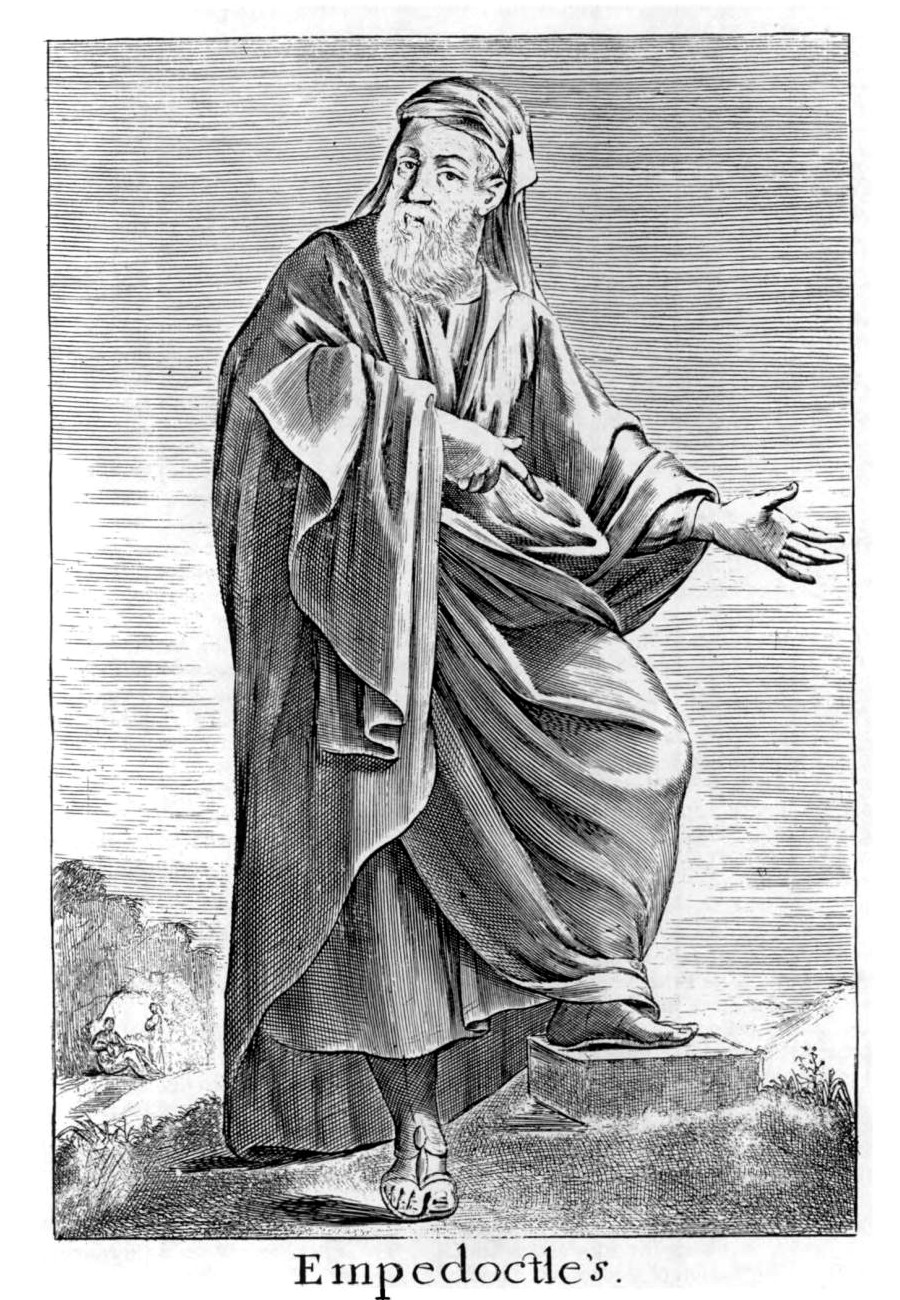
\includegraphics[width=0.4\linewidth]{./figures/empedocles.jpg}
		\caption{Empedocles \cite{Stanley1655}}
		\label{fig:empedocles}
	\end{subfigure}%
	\begin{subfigure}{0.5\textwidth}
		\centering
		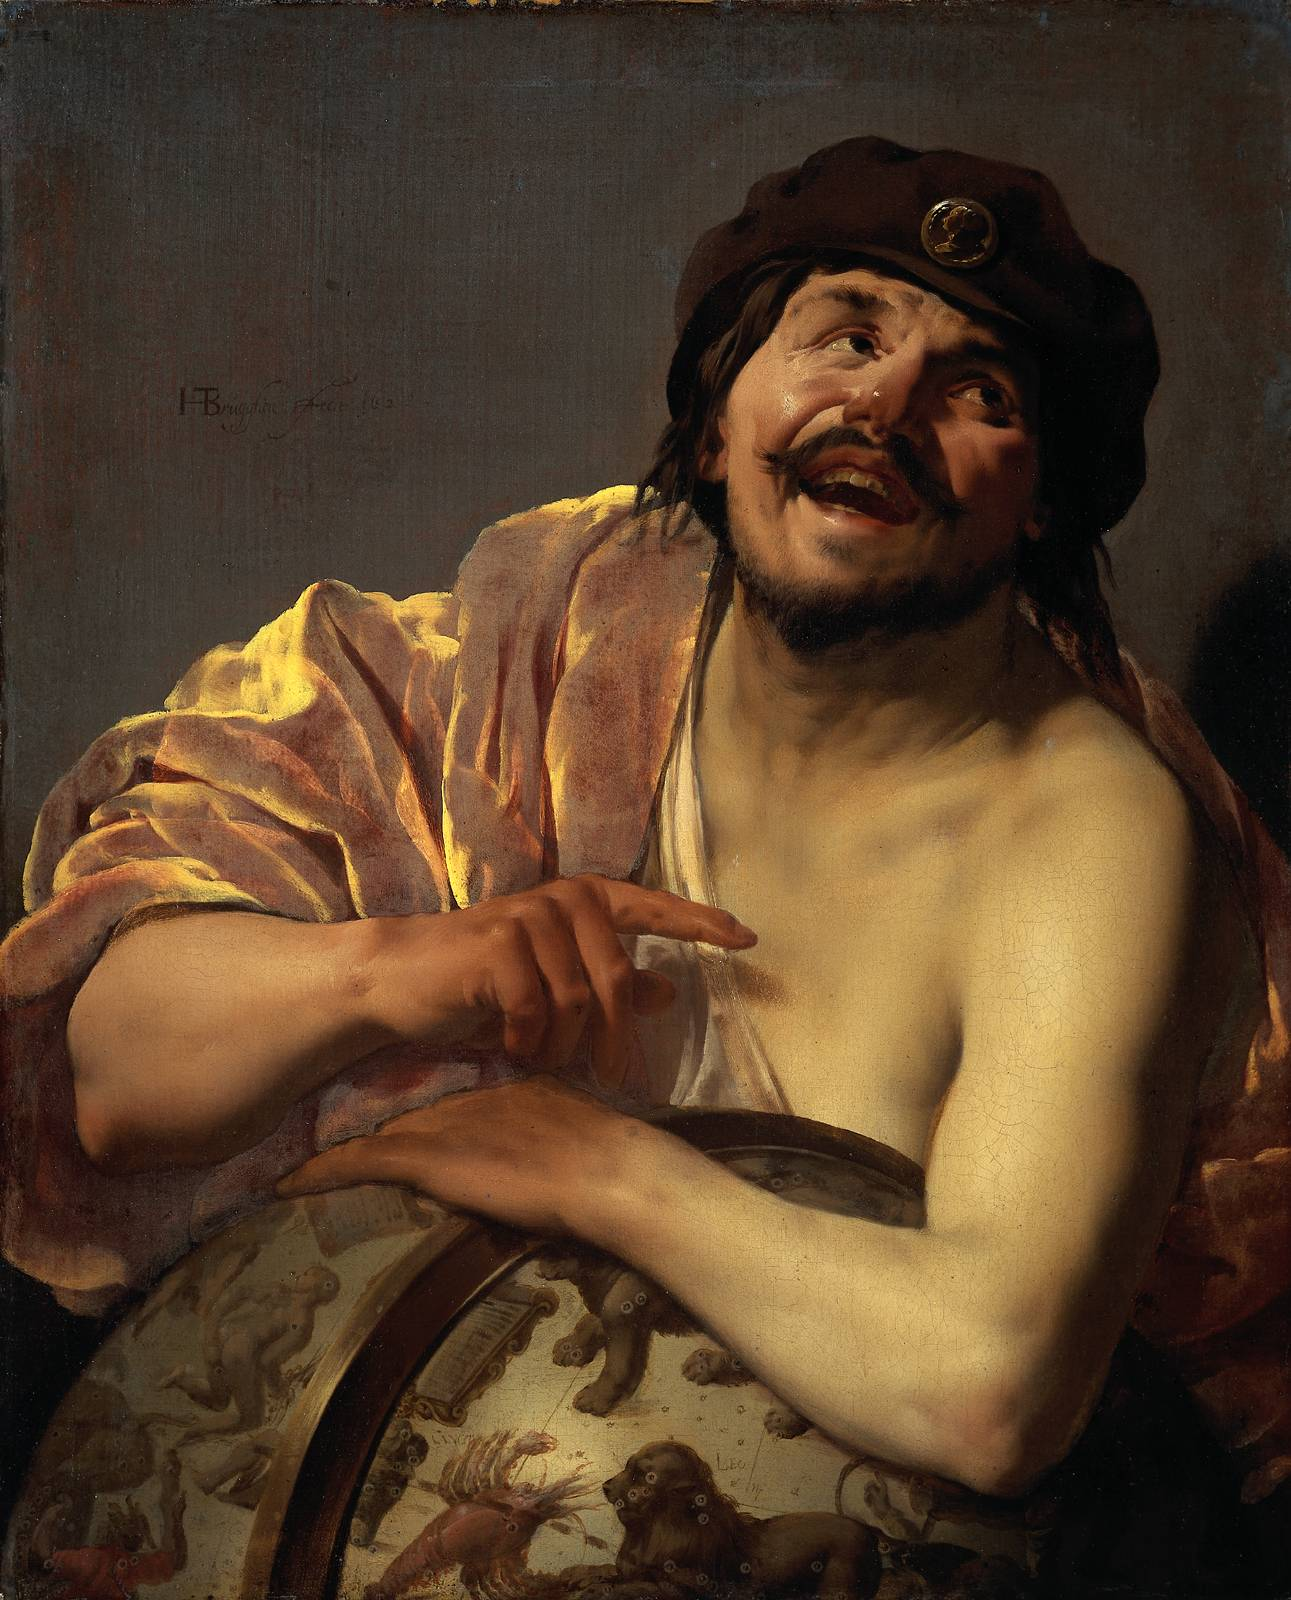
\includegraphics[width=0.4\linewidth]{./figures/democritus.jpg}
		\caption{Democritus \cite{Brugghen1628}}
		\label{fig:democritus}
	\end{subfigure}
  \caption{ 
    Two Greek philosophers, who made important philosophical contributions our
    understanding of matter. Empedocles (Panel (a)), postulated the precursor
    to the elemental theory of matter\cite{Long1949} and Democritus (Panel
    (b)), postulated the precursor to the atomic theory of matter.  
  }
	\label{fig:atomists}
\end{figure}

Democritus was part of a movement of thought which was first to make the
intellectual jump that perhaps matter was not a continuum, but instead composed
of `atomon'. `Atomon' were thought to be small and indivisible particles
building up all that is observable~\cite{Baldes1978}.  Empedocles made an
equally important philosophical stride--he posited that matter must be composed
of elemental primitives and that the properties of the primitives which build
up matter, influence the properties of the bulk matter itself~\cite{Long1949}.

Although Empedocles' `periodic table' was only composed of Earth, Water, Fire,
and Air, the idea that some unseen transmutation of elemental forces might
generate observables in nature was an important step forward. This was the
first time that humans considered that underlying structure in matter might
influence the bulk properties of matter. Proto-scientists were beginning to
generate models which derived our complicated observations from simpler forms.

\clearpage
\section{The Scientific Revolution}

Thanks to the mathematical foundations laid out by the minds of the Islamic
Golden Age (8th century - 13th century), Europe was well poised to reignite the
flames of scientific inquiry during the post Renaissance Scientific
Revolution~\cite{Alexakos2005} (17th - 18th centuries), following a renewed
interest the ideas of Greek philosophers after the dark ages.

The Scientific Revolution represented an unprecedented period of growth in
science, thanks the foundations laid during the Italian Renaissance and
emergence of British Empiricism~\cite{Cowley1968}.

\begin{figure}[ht]
	\centering
	\begin{subfigure}{.5\textwidth}
		\centering
		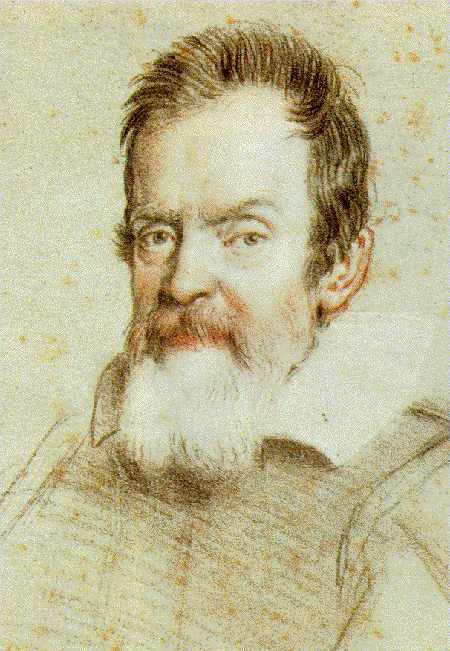
\includegraphics[width=0.4\linewidth]{./figures/galileo.jpg}
		\caption{Galileo \cite{Leoni1624}}
		\label{fig:galileo}
	\end{subfigure}%
	\begin{subfigure}{0.5\textwidth}
		\centering
		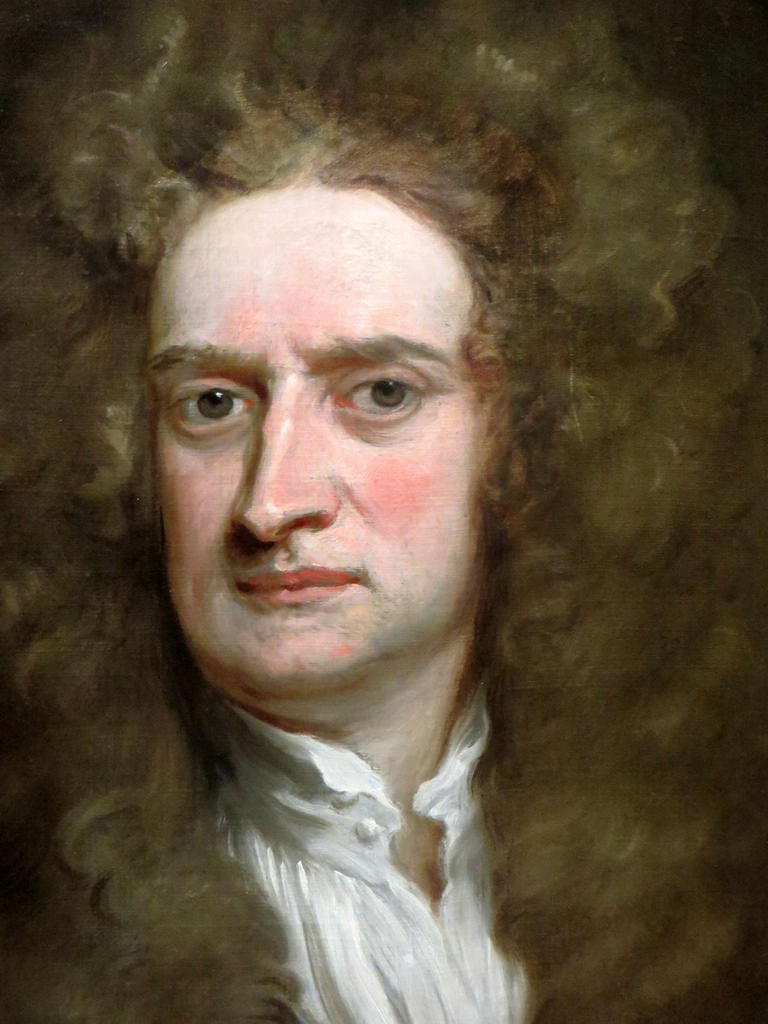
\includegraphics[width=0.4\linewidth]{./figures/newton.jpg}
		\caption{Newton}
		\label{fig:newton}
	\end{subfigure}
	\caption{ 
    Giants in the age of Empiricism, Newton (Panel (a)) and Galileo (Panel (b))
    both made foundational contributions to Physics.  Galileo lived in Italy,
    born in 1564 and dying in 1642. Newton lived in England from 1642 until his
    death in 1727
	}
	\label{fig:newtongalileo}
\end{figure}

\subsection{Galileo Galilei}

Coming at the tail end of the Italian Renaissance, Galileo brought us into the
age of Scientific Revolution.

While Galileo is best known for his work in Observational Astronomy, his
importance to science extends beyond this. During his years in exile for his
controversial views regarding the heliocentric universe, he produced some of
his most important scientific work in kinematics~\cite{Hall1965}. What made
this work remarkable is the care that Galileo took in merging mathematical
modeling with well designed experimentation. This methodical approach to
inquiry laid the foundation for the scientific method, which others would
refine. 

Galileo's formalization of the scientific method inexorably set science on a
course to delving deep into the nature of matter and the laws of nature.

\subsection{Isaac Newton}

Fittingly born in the same year as Galileo's death, Isaac Newton would carry on
Galileo's legacy of rigorous mathematical modeling mixed with experimentation.
Perhaps no other scientist has touched so many different aspects of physics,
from theories of propagation of light, to celestial mechanics, to mathematics,
and kinematics.

Newton's Principia is arguably the most important scientific work ever
published.  It opened the doors of the universe in a way that nobody has since
duplicated--Newtons' laws of motion are still taught in school today, and
applied in real scientific contexts, providing the basis for the NASA space
exploration program. Although Newton's models for motion have since been shown
to be inaccurate at the smallest and largest scales, they still provide
startlingly accurate predictions at intermediate scales.

One particularly prescient theory of Newton's was his corpuscular theory of
light. Although not his most influential theory by far, the idea that an
apparently continuous medium such as a beam of light might be made of small
packets of energy (corpuscles) turned out to be partially
right~\cite{Stuewer1970}, and gained an interesting new context with the
emergence of Quantum Mechanics in the early 20th century.

Newton's theories, and contributions to science are enormous, and have moved us
deeper still into the underpinnings of matter. It would not be until roughly 200
years after his death, in the 19th century, that we finally can take the first
steps into the world of the atomic, and sub-atomic: the world of the proton. 

\clearpage
\section{Atomic Theory}

On the shoulders of giants such as Newton and Galileo, science finally came to
know the tool which has been indispensable to modern particle physics:
scattering. Rutherford and Thompson both carried out the most important
scattering experiments in modern science. These experiments provided us with
the first hints of a hidden, quantum world. It would not be until the 20th
century that these important experiments would be fully contextualized with a
theory of quantum scattering.

Scattering experiments offer a very powerful method where one uses a well known
initial state of matter (typically in the form of a beam) and allows this beam
to interact with an unknown configuration of matter. The final state of the
target and scattered beam are measured. With a careful study of the kinematics
of the scattered beam, one can create models that offer a peak into the
structure of the target matter. As we journey down further in scale, matter
begins to look quite different.  In fact, the models we use are scale dependent,
Figure~\ref{fig:scale_of_matter}. Thomson (Figure~\ref{fig:thomsonrays}), and
Rutherford (Figure~\ref{fig:rutherford}) began to see matter as collections of
atoms.  Soon, nuclei were discovered to be divisible into protons an neutrons,
which in turn were discovered to be composed of a sea of quarks and gluons.

\begin{figure}[ht]
	\centering
	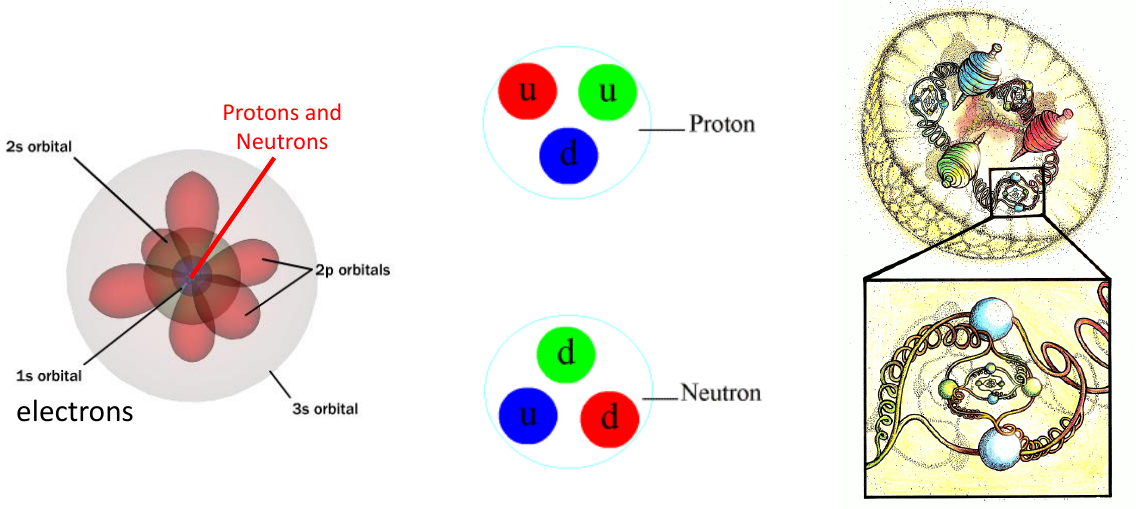
\includegraphics[width=\linewidth]{./figures/scale_of_matter.png}
	\caption{
    Matter at an atomic scale~\cite{Freudenrich2001} (left), intermediate
    nuclear scale~\cite{Manisearth2010} (center), and the sub-nuclear partonic
    scale (right)~\cite{Morreale2009}
	}
	\label{fig:scale_of_matter}
\end{figure}

\subsection{John Dalton}

While many had postulated the existence of atoms, the first evidence based
theory which suggested the existence of atoms was produced by John Dalton in the
early 19th century. Dalton made an important conceptual leap to relate the
existence of stoichiometric ratios in chemistry to the presence of small,
individual functional units in his experiments with chemical reactions.
Dalton's realization was only made possible due to his careful accounting of
reactants in his experiments.

However, humanity had to wait for Einstein's 1905 theory on Brownian Motion to
be experimentally verified by Jean Perrin to obtain the first limits on the mass
and size of atoms that Dalton's atomic theory predicted~\cite{Patterson200750}.

\subsection{J.J. Thompson}

\begin{figure}[ht]
	\centering
	\begin{subfigure}{.4\textwidth}
		\centering
		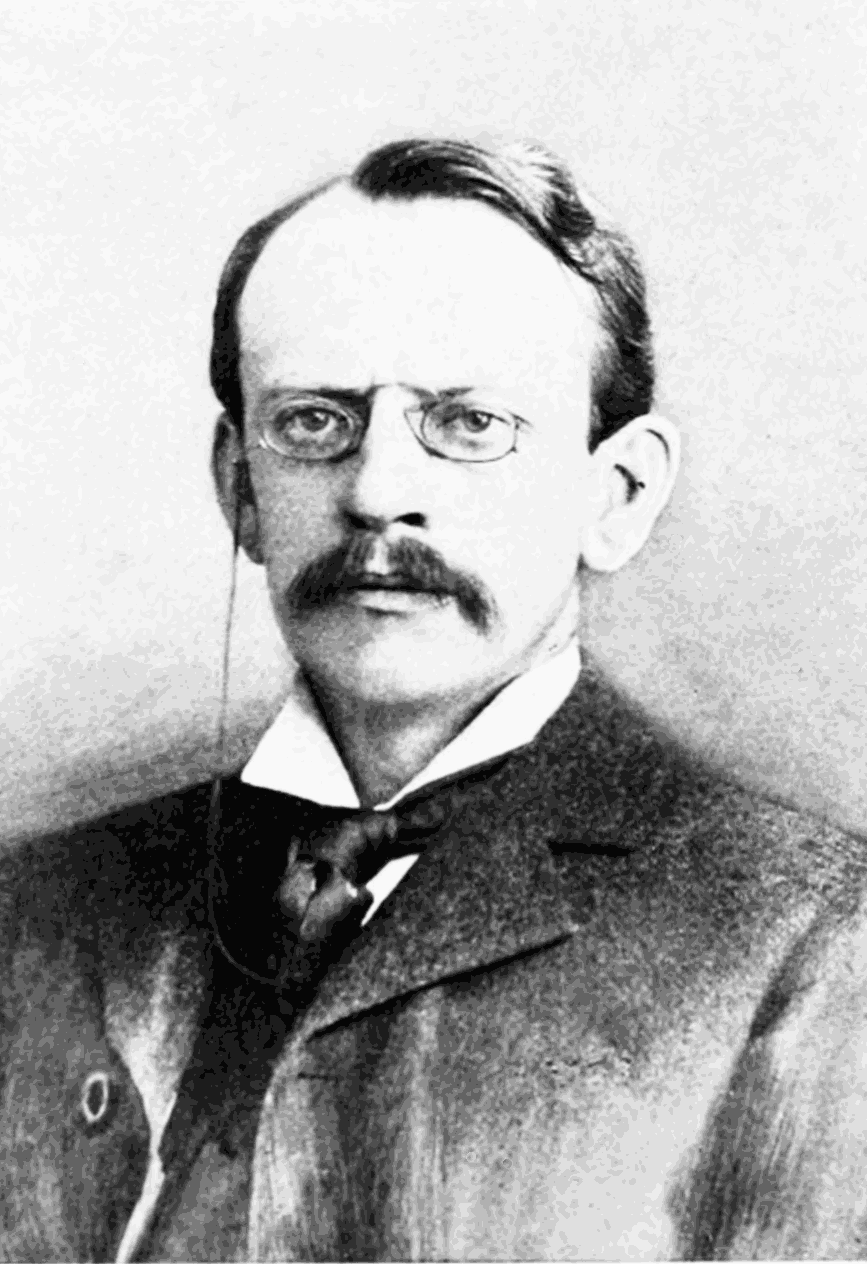
\includegraphics[width=0.4\linewidth]{./figures/jjthomson.png}
		\caption{J.J. Thomson  \cite{PopularScience1899}}
		\label{fig:thomsonportrait}
	\end{subfigure}%
	\begin{subfigure}{0.6\textwidth}
		\centering
		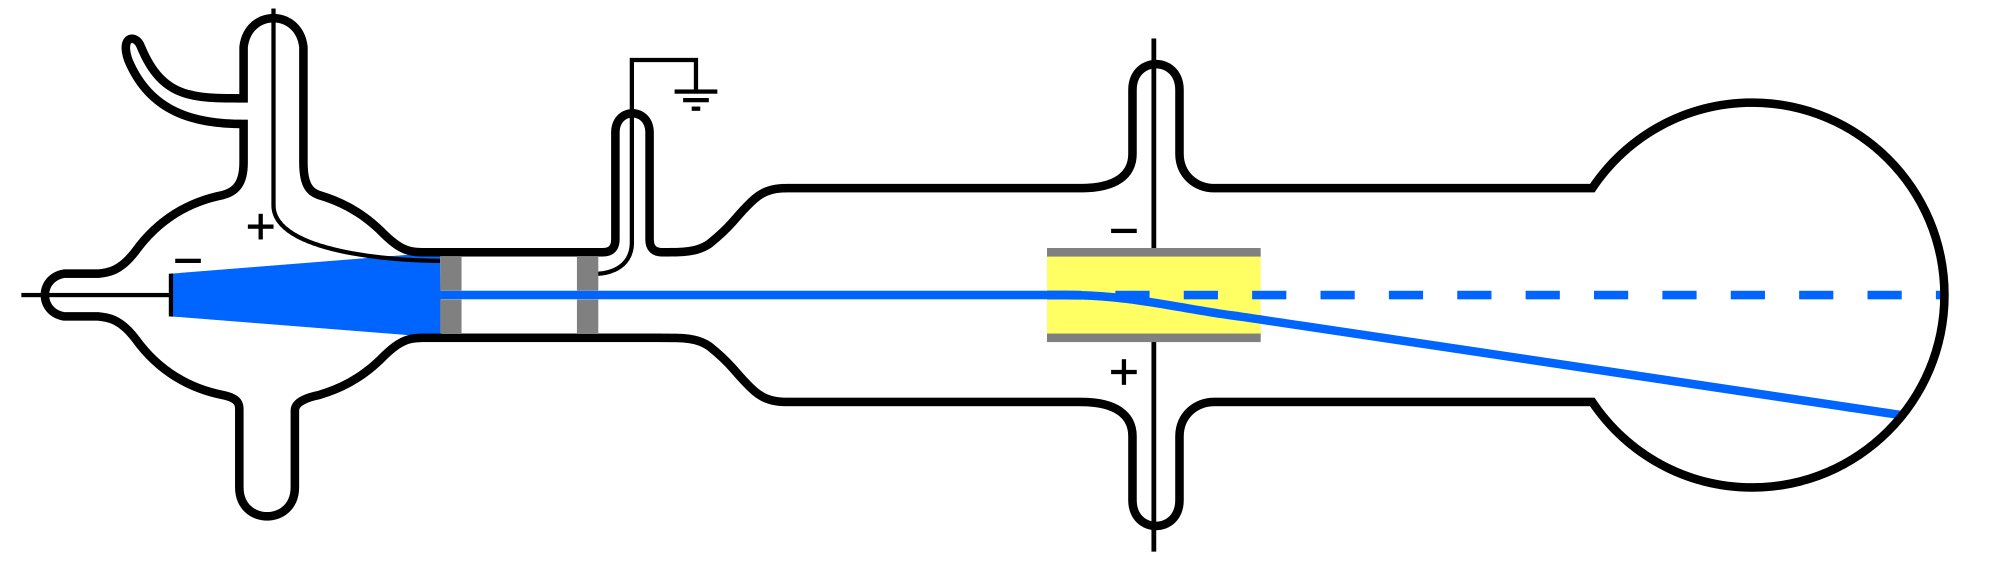
\includegraphics[width=0.4\linewidth]{./figures/cathoderaytube.png}
		\caption{Cathode Ray Tube  \cite{Kurzon2010}}
		\label{fig:thomsoncathode}
	\end{subfigure}
	\caption{ 
		Left: J.J. Thomson, who showed that cathode ray tubes were in fact producing
		the first observed subatomic particle: the electron. Right: A cartoon of
		Thomson's cathode ray tube setup. Electrons would be deflected by a magnetic
		field, sent from cathode to anode.
	}
	\label{fig:jjthomson}
\end{figure}

Thomson (Figure~\ref{fig:jjthomson}) would discover that atoms are not the
smallest indivisible piece of matter. In his landmark experiment, he used
cathode ray scattering experiments to show that cathode rays were in fact
subatomic particles. He showed these cathode rays were identical to particles
given off by the photoelectric effect. He discovered that these were the same
particles responsible for electric current.  Scientists began to wonder: if
atoms were not the smallest piece of matter, then perhaps atoms themselves
might not be `indivisible' as previously thought \cite{nobelthomson2014}.

\subsection{Ernest Rutherford}

\begin{figure}[ht]
	\centering
	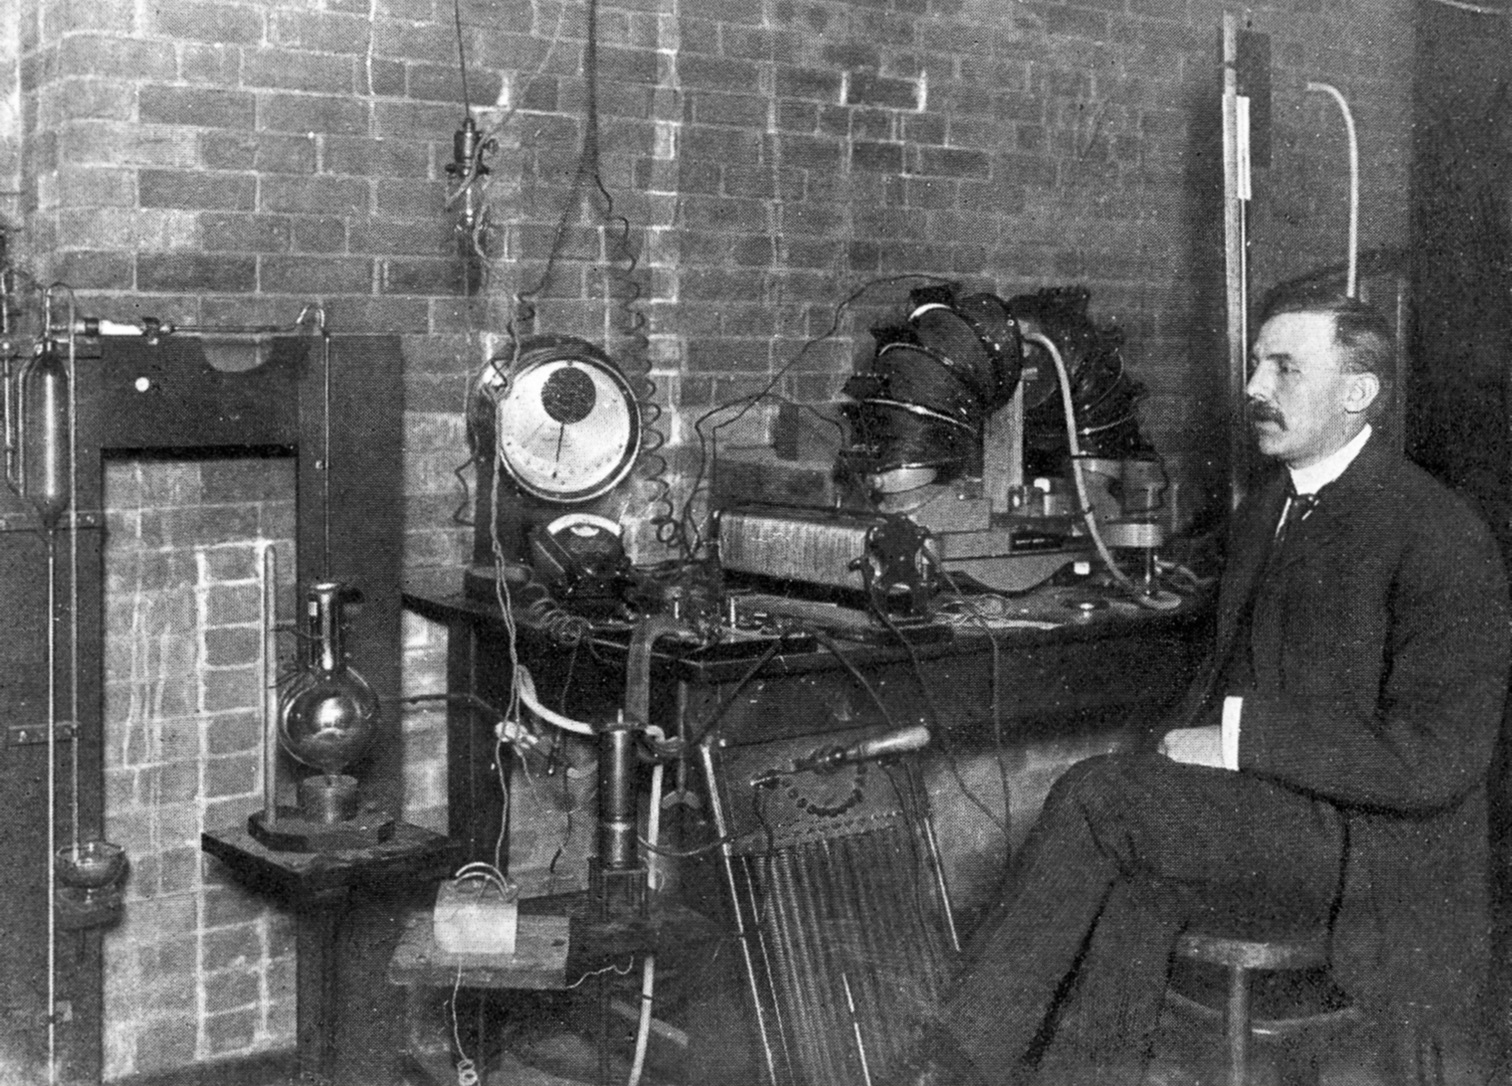
\includegraphics[width=0.6\linewidth]{./figures/ernestrutherford.jpg}
	\caption{Ernest Rutherford, in his lab.  \cite{Eve1939}}
	\label{fig:rutherford}
\end{figure}

Ernest Rutherford (Fig~\ref{fig:rutherford}) was the first to show that atoms
themselves had underlying structure and consisted of a small dense center.  He
had discovered the nucleus.

\begin{figure}[ht]
	\centering
	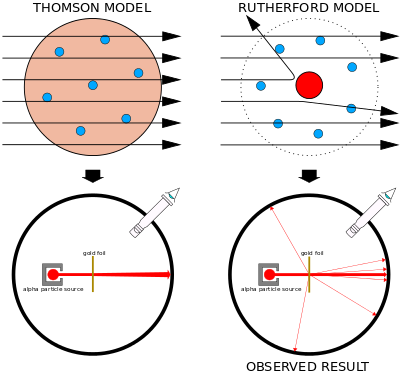
\includegraphics[width=0.6\linewidth]{./figures/geiger_marsden.png}
	\caption{
		Ernest Rutherford's historic experiment, showing (top right) that atoms were
		composed of a small dense nucleus, in contrast to Thomson's `pudding model'
		of homogeneous charge (top left). The experiment, (bottom left and right)
		contrast the expected results (bottom left) against the observed results
		(bottom right)  \cite{Kurzon2014}.
	}
	\label{fig:geigermarsden}
\end{figure}

Rutherford's work with radioactivity was of fundamental importance. He
discovered and classified both alpha-particle radioactivity and beta-particle
radioactivity. Further studies into these types of nuclear radiation would
unlock the nucleus of atoms through the work of future scientists.

After his discovery of the proton, Rutherford proposed a planetary model for the
nucleus. While this model was eventually shown to be wrong, it shifted paradigms
from the pudding model of atoms to the more familiar nucleus + electron model.
This shift eventually led to the emergence of Quantum Mechanics.

Rutherford's work helped push us out of the cocoon of classical mechanics into
the world of the quantum mechanics--scientists would soon find that the nucleus
is not just a dense concentration of charge, but a probabilistic structure, with
rich sub nuclear structure.

\clearpage
\section{Early Quantum Theory}

During Rutherford's time, experiments were already underway investigating
modeling light as a wave phenomena. This was in contrast to Newton's
(unverified) corpuscular theory of light. The argument whether light was
wave-like or particle-like eventually lead to a classical field theory
describing light as electromagnetic radiation. Max Planck proposed theories
which required the quantization of light~\cite{Planck1901}.  Einstein would show
that light is indeed quantized into packets of energy in his analysis of the
photoelectric effect. The nascent atomic theory of matter hinted at a hidden,
quantized world.

\begin{figure}
	\centering
	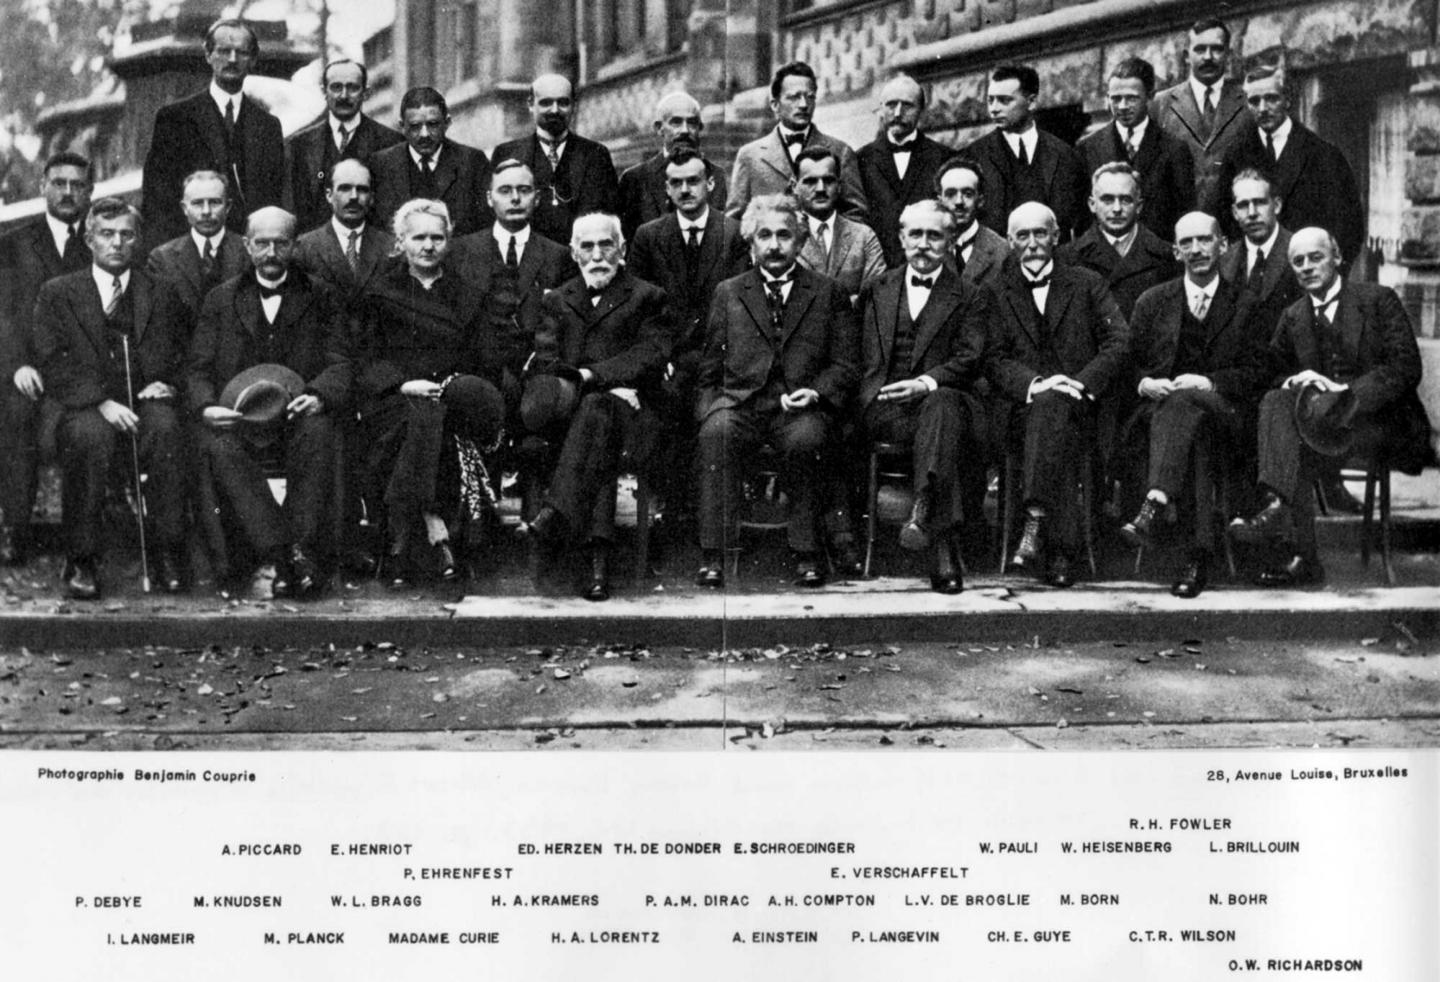
\includegraphics[width=\linewidth]{./figures/solvay.jpg}
	\caption{
		The attendees of the Solvay Conference in Brussels, 1927
		 \cite{BenjaminCroupie1927}.
	}
	\label{fig:solvay}
\end{figure}

At the 1927 Solvay Conference in Brussels(Figure \ref{fig:solvay}) an
unprecedented gathering of some of the most important figures in modern physics,
built the foundations of what would become quantum mechanics. These scientists
defined the nature and rules of quantum mechanics--the weird model which
accommodates a wave-particle duality of matter. 

It was found that not only light possesses this wave-particle duality, but also
the particles that make up atoms. These models were formalized by Paul Dirac,
David Hilbert and John Von-Neumann.

Further refinements and additions to quantum mechanics gave birth to quantum
field theory. Early quantum models were very successful at describing static
particles trapped in static potentials. Scientists could predict exactly
observed atomic emission spectra. But, more work was needed to understand the
relationship between electrical currents, light and magnetism.  These concepts
were all related by James Clerk Maxwell~\cite{Maxwell1865} in the latter half of
the 19th century, but had yet to receive a quantum-treatment.

Dirac was first to create a model for describing the electron, its behavior in
electromagnetic fields, and photon emission and absorption. Dirac's models were
fully relativistic~\cite{Dirac}. Dirac's model was so successful, that it would
become the basis for what we now call quantum electrodynamics.  Much of the
mathematical formalism was reused to describe other field theories. Field Theory
is the ultimate language used in modeling and describing the structure of
matter--including the insides of a proton. 

\begin{figure}[ht]
	\centering
	\begin{subfigure}{.4\textwidth}
		\centering
		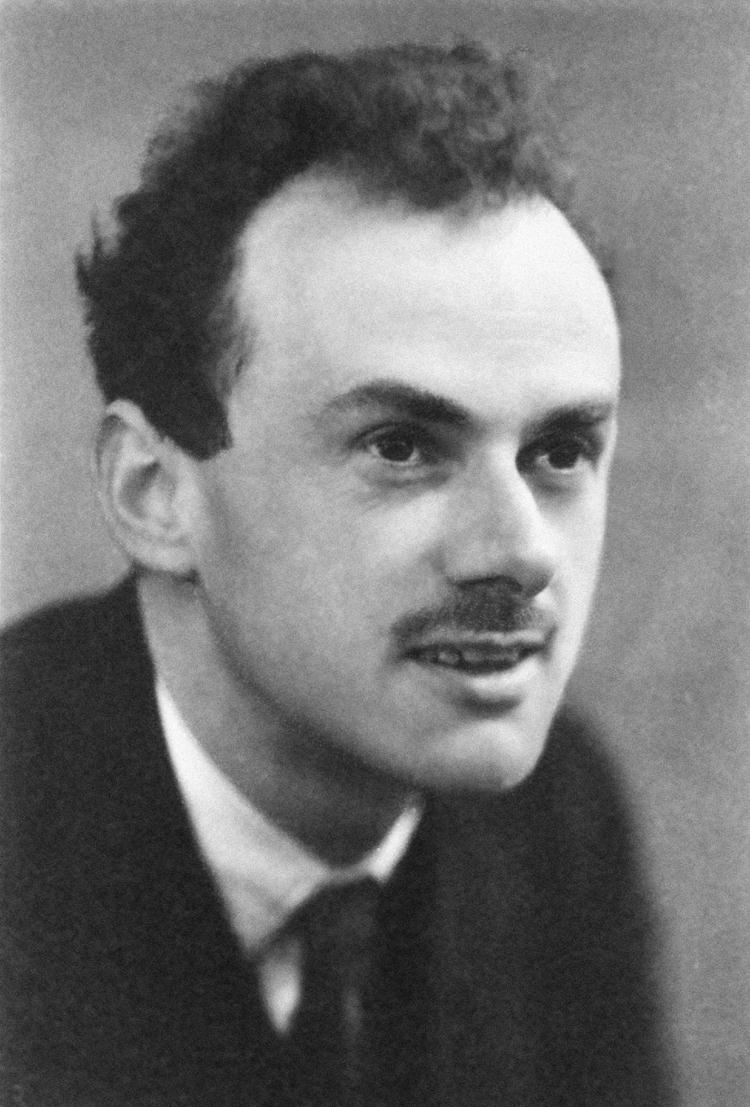
\includegraphics[width=0.4\linewidth]{./figures/pauldirac.jpg}
		\caption{Paul Dirac, 1933  \cite{NobelFoundation1933}}
		\label{fig:pauldirac}
	\end{subfigure}%
	\begin{subfigure}{0.6\textwidth}
		\centering
		\begin{equation}
			\left(\beta mc^2 + c\left(\sum_{n \mathop =1}^{3}\alpha_n p_n\right)\right) \psi (x,t) = i \hbar \frac{\partial\psi(x,t) }{\partial t}
		\end{equation}
		\caption{The `Original Form' of the Dirac Equation}
		\label{eq:diracquation}
	\end{subfigure}
	\caption{ 
		Paul Dirac, next to his original formulation of the Dirac Equation,
		describing the wave function for an electron with rest-mass $m$, in terms of
		its space-time coordinates. Dirac's equation has been expressed free of any
    defined basis.
	}
	\label{fig:thomsonrays}
\end{figure}

Dirac's work successfully merged relativity into his wave equations describing
the motion of particles. He additionally incorporated the spin (i.e. Dirac
Spinors) of these particles. The inclusion of spin allowed for the most precise
predictions ever to be made for hyperfine divisions in the atomic
spectra~\cite{Dirac}.

In Dirac's time, the proton was already known to reside in the enigmatic
nucleus. However attempts to use Quantum Electrodynamics to describe the state
of the nucleus failed. It was clear that there was a very strong force holding
together the positively charged protons of a nucleus. This force would have to
be far stronger than the electromagnetic repulsion felt by the positively
charged particles in such close proximity. Further complicating an understanding
of the nucleus is the fact that as the length scale of probing decreases, the
energies probed increase. This fundamentally makes the nucleus a relativistic
object. Physics would once again forge ahead in attempting to understand the
inner workings of the nucleus.

\clearpage
\section{Early Particle Physics and The Eightfold Way}

The hydrogen atom and its spectra was well-modeled with quantum mechanics by the
end of the early 20th century. However, attempts to study Helium were not as
successful. By 1932, when James Chadwick turned a beam of helium particles (at
that time only known as $\alpha$ particles) on a sample of Beryllium, he
observed that neutral, non-ionizing, penetrating radiation was produced
\cite{Krauss2015}.  Photons were ruled out as possible candidates, leading to
the discovery of the neutron. Protons and neutrons were hypothesized by
Heisenberg to both be the same state of a new conceptual particle, the
nucleon~\cite{Heisenberg1952}. In the same year, Carl Anderson discovered the
positron. 

By 1934, Hideki Yukawa (Fig.~\ref{fig:hidekiyukawa}) had created an effective
field theory for interactions of `elementary particles' (at this time, thought
to be protons and neutrons). He predicted the existence of mesons, and wrote
down an effective field theory which described how protons and neutrons bind
together in the nucleus \cite{Yukawa1935}. 

Though non-relativistic quantum mechanics was mostly complete by 1934,
scientists were already hard at work incorporating relativistic corrections to
the theory. Experiments with cosmic rays soon revealed the existence of muons
and the first observation of mesons.

\begin{figure}[ht]
	\begin{center}
		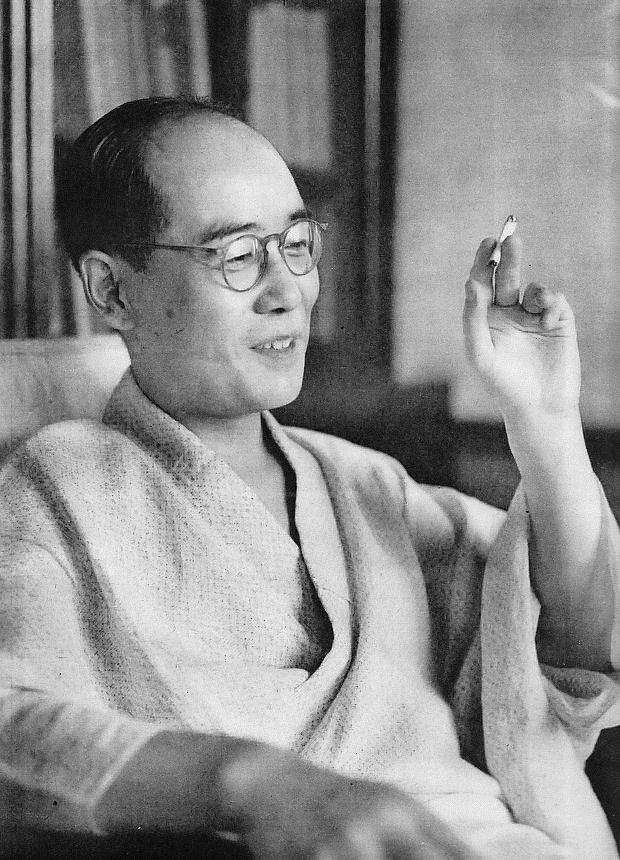
\includegraphics[width=0.5\linewidth]{./figures/hidekiyukawa.jpg}
		\caption{
			Hideki Yukawa, the first Japanese Nobel Laureate and publisher of
			influential research on the theory of mesons, and other elementary
			particles  \cite{YukawaPhoto1952}.
		}
		\label{fig:hidekiyukawa}
	\end{center}
\end{figure}

Three separate paths eventually lead to the development of particle
accelerators. To date, these massive machines provide the best apparatus in
physics to probe nuclear structure. These accelerators are an outgrowth of ever
more intense Rutherford-style experiments. An array of technologies have
supported this growth: Tandem Van-Der-Graaf generators, resonant acceleration
techniques, RF linacs, and betatron accelerators \cite{Bryant1994}.

By the 1950s a cornucopia of strange new particles had been discovered, both
matter and antimatter. Neutrinos were proposed as a means of understanding
`missing energy' observed in some scattering experiments. Mesons such as Kaons
($K$), Pions ($\pi^+,\pi^-,\pi^0$), and Lambdas ($\Lambda$) were well
understood.  Physicists were doing nuclear chemistry, attempting to work out how
quickly some particles decayed, and what decays were allowed or forbidden.
Science entered an age of nuclear alchemy.

``Strange'' particles were discovered ($K$ and $\Lambda$), so called because in
bevatron experiments, they were produced in great quantities, but were slow to
decay, unlike the faster $\pi$ decay. Gell-Mann proposed that this strangeness
in matter was due to a new quantum number (he called it `strangeness'). The name
stuck~\cite{Gell-Mann1953}, \cite{Gell-Mann1956}, \cite{Krauss2015}.

The introduction of new conserved quantities and the vast proliferation of
particles was an exciting puzzle for physicists to unravel. The subatomic world
of the 1950s was confusing and complex. In his book, \textit{The God Particle},
Leon Lederman recalled his adviser (Enrico Fermi) frustratedly remarking `Young
Man, if I could remember the names of these particles, I would have been a
botanist'.  At this time the number of mesons and baryons that had been
discovered were at least in the dozens, if not more.

While the use of particle accelerators were speeding along the scientists' quest
to understand structure of matter, one particular invention truly revolutionized
the field--the bubble chamber (Figures~\ref{fig:bubble_chamber} and
~\ref{fig:bubble_tracks}).

The bubble chamber is essentially a large vat of supercritical fluid which could
easily be caused to boil with small perturbations. This feature was exploited,
by positioning a bubble chamber in a magnetic field (to cause charged tracks to
bend) near the interaction point between a particle beam and a fixed target. The
bubble chamber itself was sometimes the target--since a popular liquid to use
was hydrogen. 

\begin{figure}[ht]
	\centering
	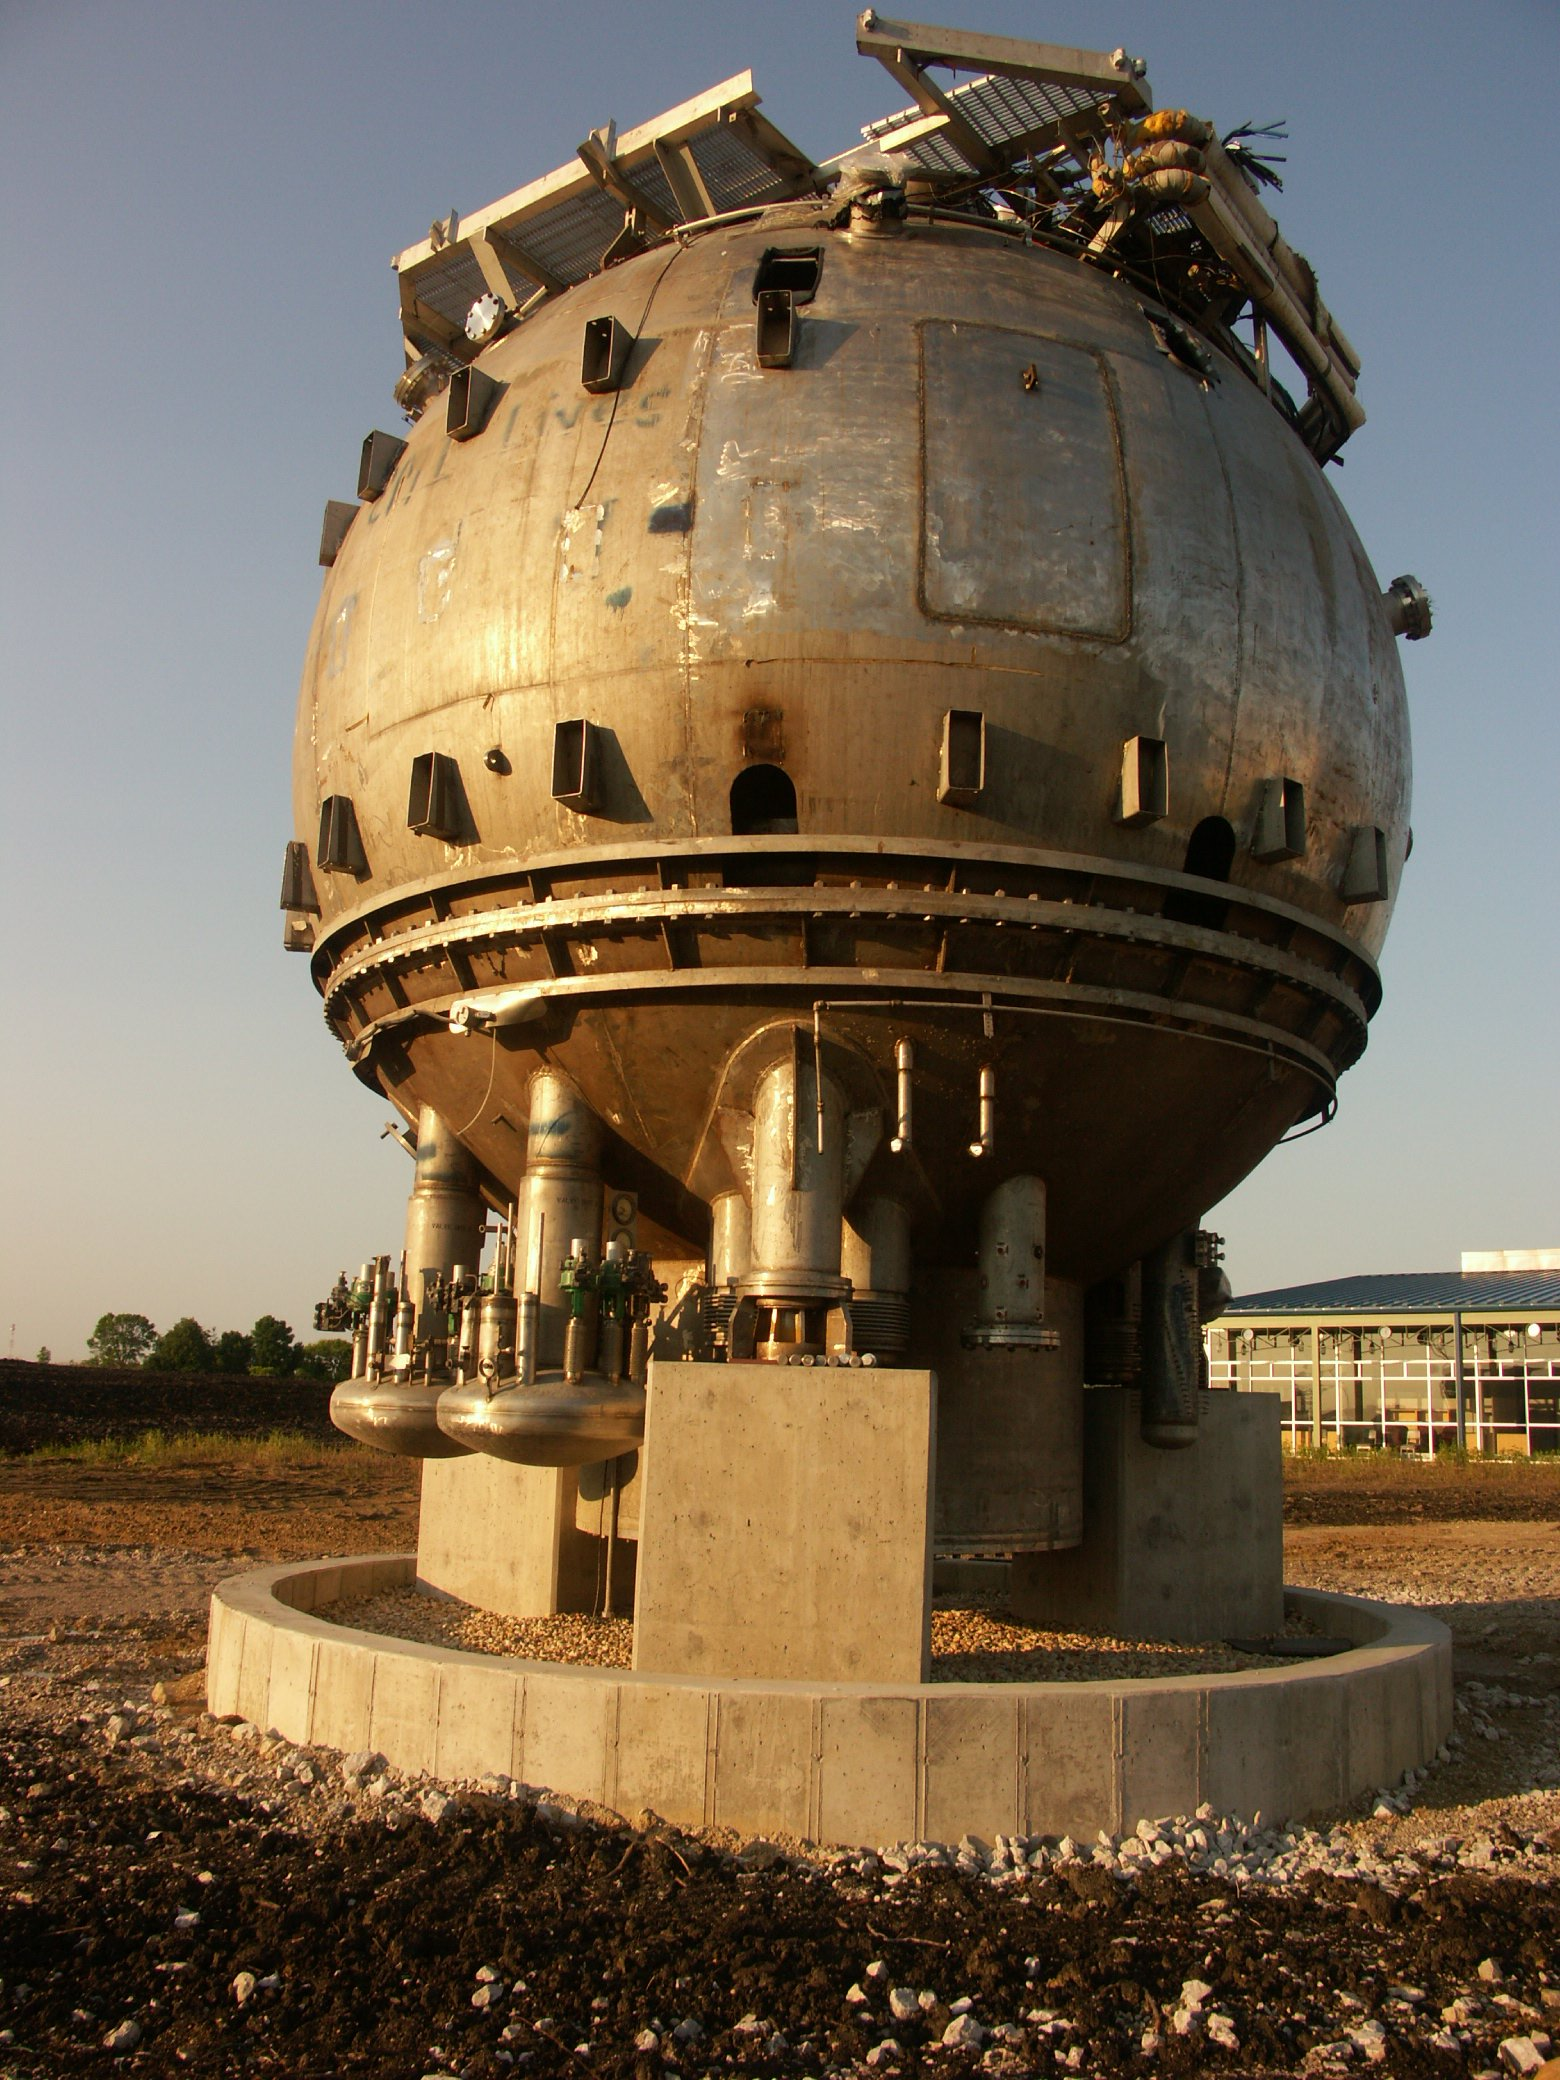
\includegraphics[width=0.5\linewidth]{./figures/bubblechamberfnal.jpg}
	\caption{An old bubble chamber, once used at Fermilab,
	 \cite{FNALBubbleChamber2005}}
	\label{fig:bubble_chamber}
\end{figure}

Invented by Donald Glaser in 1952, the bubble chamber was `perfected' by Luis
Alvarez when he helped to develop a version which could be used with liquid
hydrogen. Hydrogen was desirable as a target and medium due to its simple
structure. This led to cleaner results, unlike the original medium Ether.
Additionally, using hydrogen gave physicists a convenient way to directly probe
the sub-nuclear structure of the simplest form of matter.

\begin{figure}[ht]
	\centering
	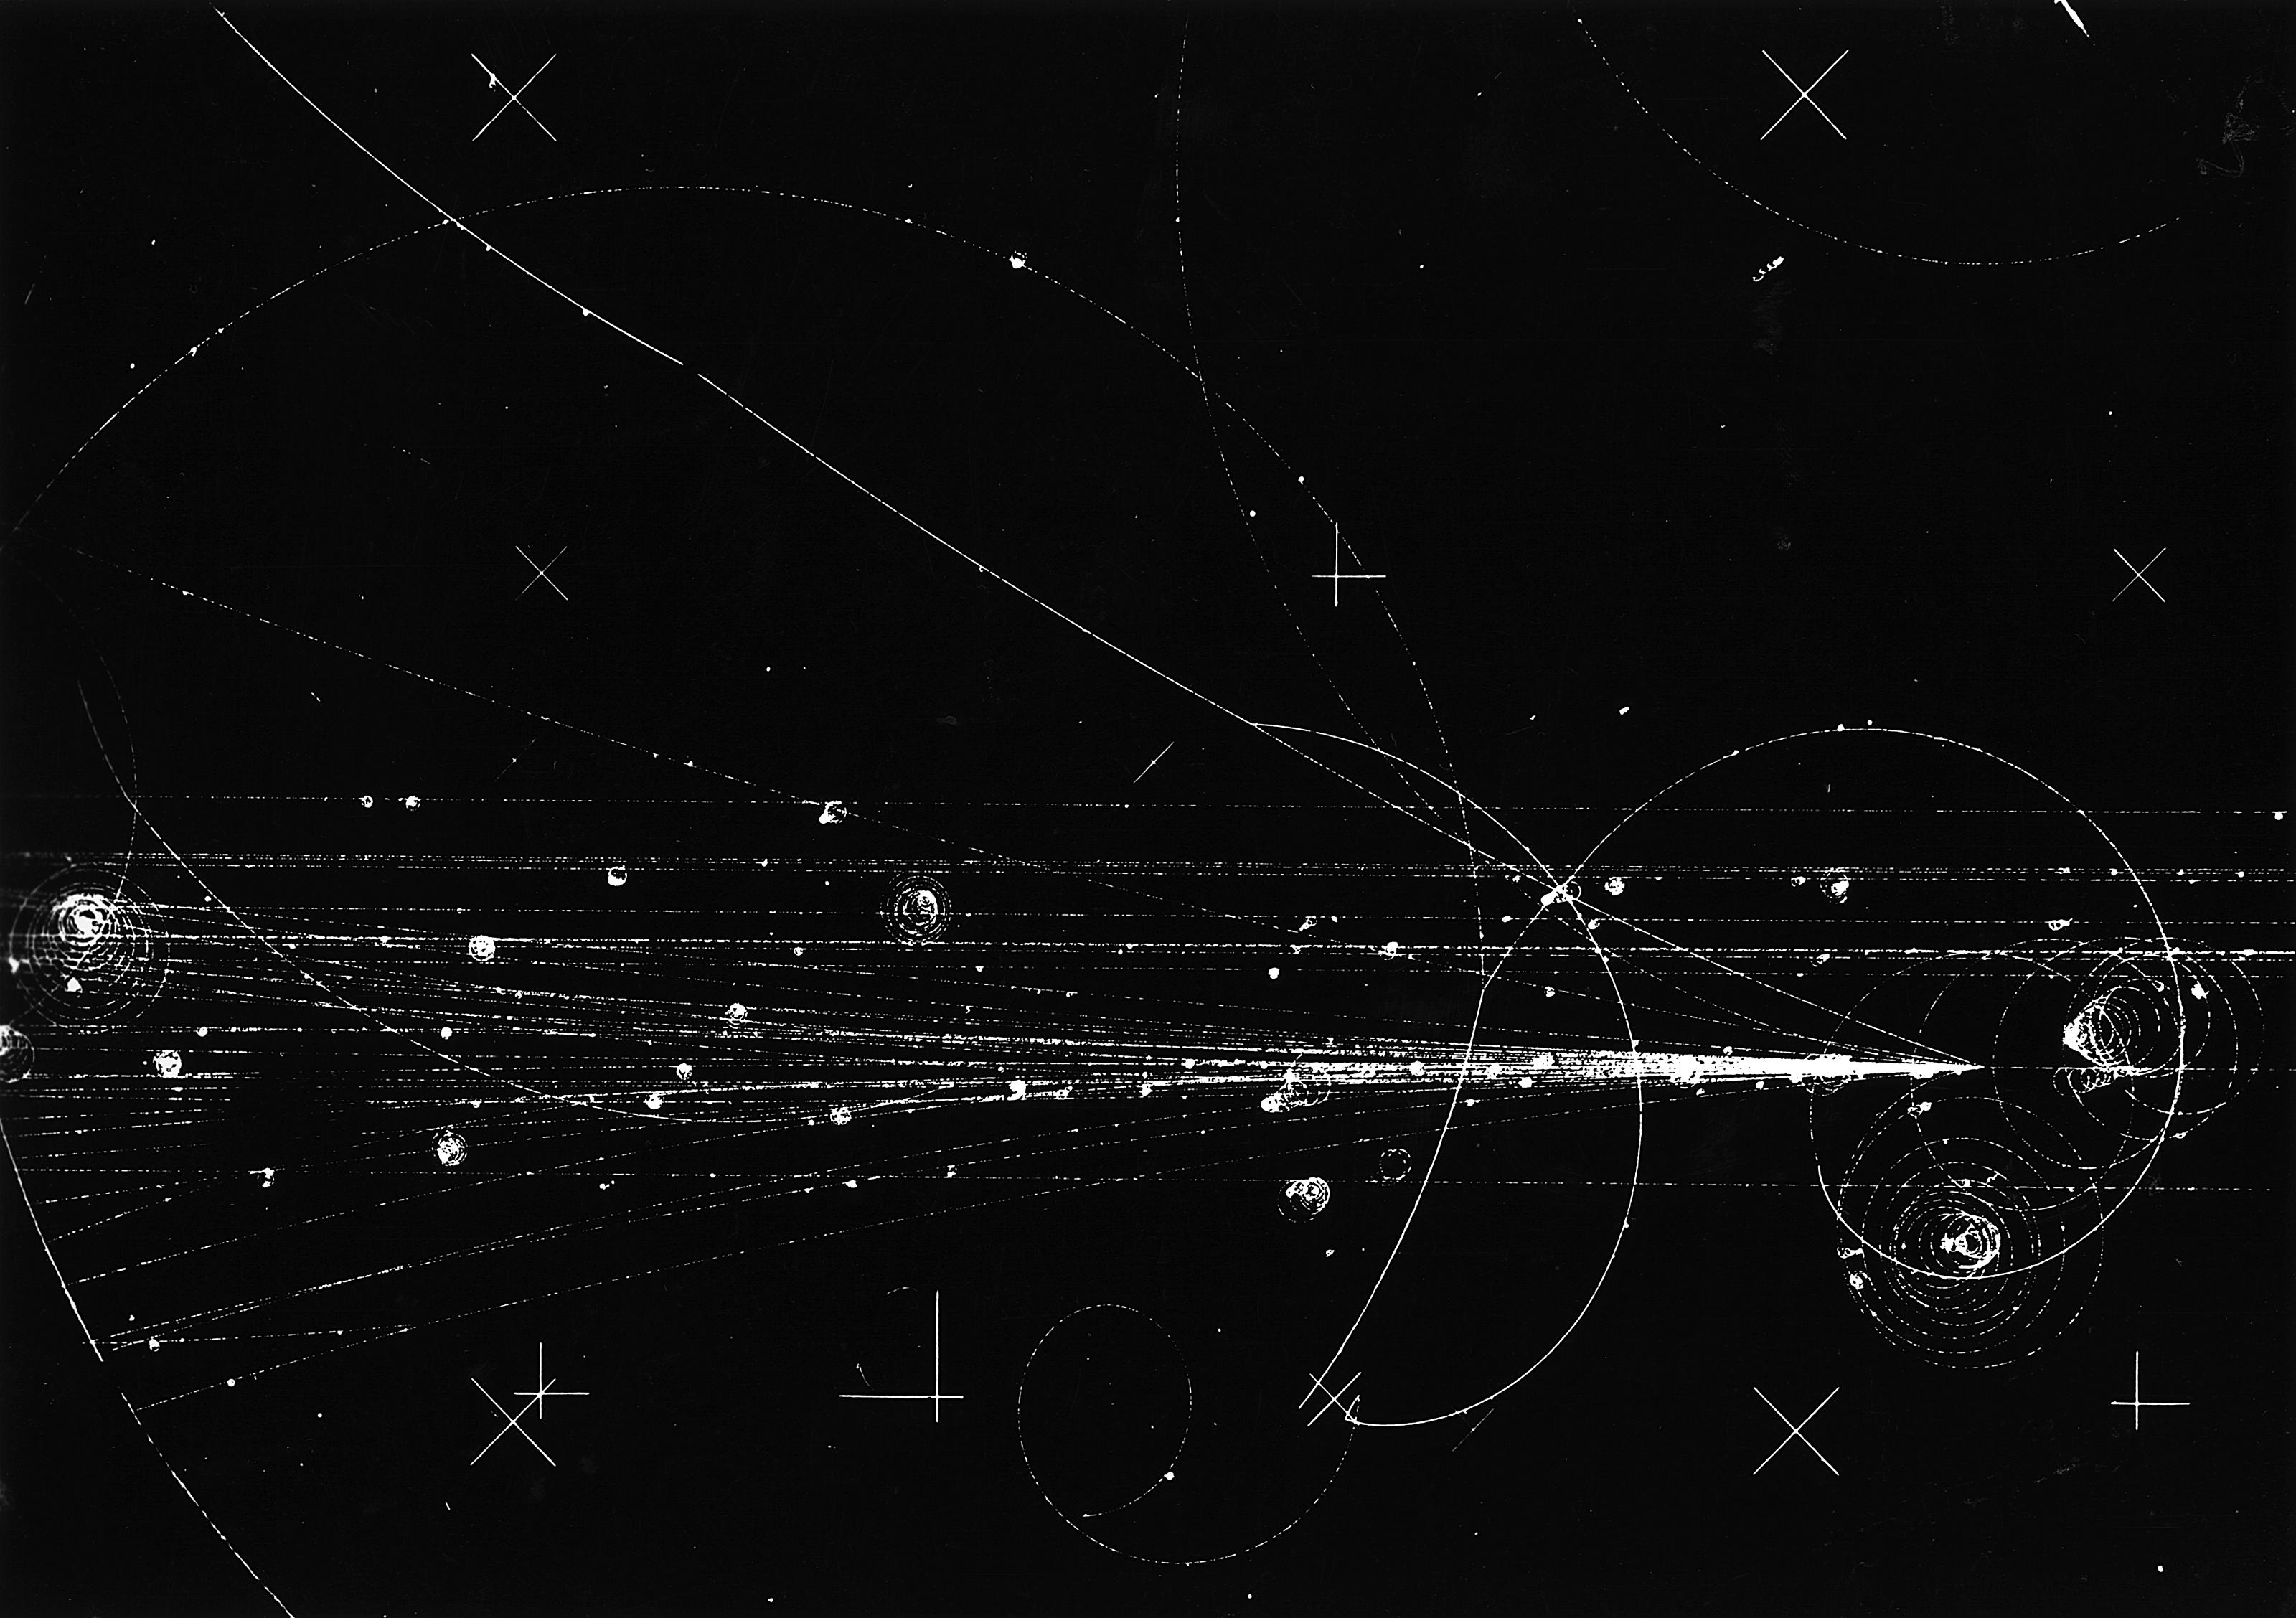
\includegraphics[width=0.5\linewidth]{./figures/bubble_chamber_tracks.jpg}
	\caption{
		An example of the photographs taken with a Bubble Chamber, in 1973.
		In this picture, we see a 300 $GeV$ proton producing particles as it travels
		through a hydrogen-filled bubble chamber at Fermilab  \cite{HD6B235}.
	}
	\label{fig:bubble_tracks}
\end{figure}

Soon after the advent of bubble chambers, physicists were able to
macroscopically image these new, exotic particles interacting with normal matter
and decaying. Novel computer techniques were developed to analyze and catalog
the massive influx of data.

A break-through came in 1961, when Gell-Mann and Nishijima recognized the
underlying symmetry of the interactions taking place and created what would be
known as `the eightfold way'. This theory created a scheme for organizing the
observed baryons and mesons according to their properties in groupings called
``octets''. These octets were in fact representations of the elements of members
of the $SU(3)$ group. Gell-Mann had discovered the underlying structure of
flavor-symmetry between the three lightest quarks--$u$, $d$, and $s$. 

Gell-Mann's quark model soon made important predictions which were later
verified, notably the existence of the $\Omega^{-}$ mesons, the ground-state
particle of the spin-$3/2$ decuplet, discovered at Brookhaven National
Laboratory. Gell-Mann formalized his quark theory of matter in 1964, however,
due to the unforeseen phenomena of color confinement, it would be several years
before evidence of quarks composing baryons and mesons was directly obtained
from deep inelastic scattering experiments.

This work directly led to the development of the quark model of matter and the
foundation of what would become the foundation of the standard model of
particles. To date, the standard model is the most successful theory describing
particles and their interactions.


\clearpage
\section{Deep Inelastic Scattering, Quantum Chromodynamics and The Parton Model}

Deep inelastic scattering experiments (Figure~\ref{fig:disschematic}) were a
natural outgrowth of Rutherford's experiment from the late 19th century.
Rutherford's scattering experiments can be modeled classically, by using a
classical potential as a scattering source. One solves as usual using an
impact parameter and potential as in central force problems.  Rutherford's
experiments were considered generally `elastic' because the target absorbed very
little kinetic energy from the projectile, and no new particles were created
from the kinetic energy of the projectile-target system.

By the late 20th century, scattering experiments became highly inelastic.
Targets would absorb a lot of kinetic energy, sometimes so much that targets
would break apart and the kinetic energy of the system would create particles.

Deep Inelastic scattering describes the process in which a high energy
interaction occurs between a projectile (often a beam) and a target (a gas, or
another beam). The process is akin to smashing to swiss-watches together to
understand how the gears fit together in synchrony to tell time. 

The interaction occurring between the target and the projectile can change the
state of the projectile and generate matter due to the high energies involved.
One can observe the state of the projectile and account for the matter which is
created.  If there are laws which govern how the state of the projectile changes
or the kinds of matter that can be created, then we can run the clock backwards
and reconstruct the initial state from the final state of the interaction.
Alternatively, the goal of deep inelastic scattering may also be to simply
measure and characterize the final state of an interaction, based on a known
initial state. This process teaches us something about nuclear structure (or
even partonic structure). In this way, one can also identify conserved
quantities, which in turn suggest physical symmetries and help to build models.

One can think of an interaction of a beam and target in terms of a probability
of interaction. One can mathematically `separate' part of this interaction
probability into a quantity called a 'cross-section', often denoted as $\sigma$
for a total cross section, or $d\sigma$ for a differential cross section, or
even ${d\sigma}\over{d\Omega}$ to refer to a differential cross section
scattered into a solid angle. Understanding the cross-section of a process
requires knowledge of the luminosity (interactions per second, per unit area) of
beam with respect to the target. Understanding Luminosity is of fundamental
importance, and is discussed in Chapter~\ref{ch:vernier_analysis}.

A subcategory of deep inelastic scattering is 'Semi-Inclusive Deep-Inelastic
Scattering'. This refers to a case where a beam (say a lepton, such as an
electron) interacts inelastically with a point-like internal structure of a
target particle, and a hadron is produced (such as a $\pi^+$), which is then
detected. Semi-Inclusive Deep-Inelastic scattering is then the process by which
the scattered lepton and a specific hadron are measured in the final state of
the interaction (but other particles that might be produced are neglected or
ignored).

Nuclei are not elementary particles. They are built up from what we assume are
fundamental particles. Deep inelastic scattering experiments slowly revealed
that individual protons and neutrons are not elementary particles, but instead,
composite particles.  It is natural to assume that the properties of protons and
neutrons are not `fundamental' either, in that these properties must be emergent
from the partonic substructure. In fact, the vast zoo of particles that were
discovered in early inelastic scattering experiments, such as $\pi$ or $K$, or
any meson or baryon are not fundamental, but bound states of quarks and gluons.

\begin{figure}[ht]
	\centering
	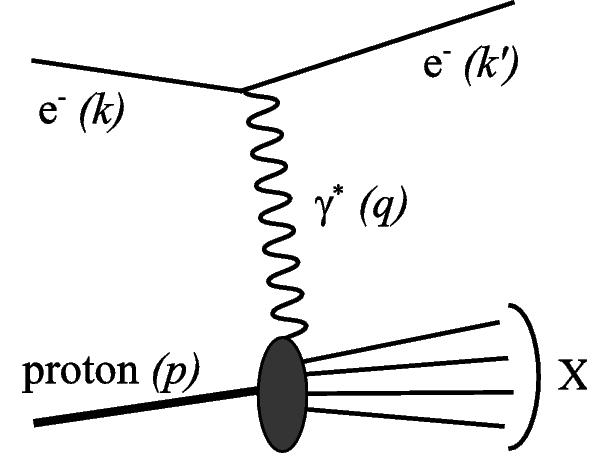
\includegraphics[width=0.6\linewidth]{./figures/deep_inelastic_basic.png}
	\caption{
    A schematic~\cite{Ddn2_2008} of deep inelastic scattering, where the
    incoming electron inelastically scatters off the proton, producing results
    $X$, via virtual photon exchange, $\gamma^*$. The diagram is split into a
    perturbative portion (the electron) and a non-perturbative portion.
    Mathematically, we describe the interaction with kinematic variables
    summarized in Equations~\ref{eq:P}-\ref{eq:x}
  }
	\label{fig:disschematic}
\end{figure}

By the 1970s, collaborations between Bjorken, Feynman, and others had produced
a coherent partonic model which contained quarks and force-mediating gluons.
The concept of Structure functions had been developed. Modified from
Rutherford's original scattering formula, a new formalism to describe the cross
section of deep inelastic scattering incorporated structure functions. Structure
Functions provide a means to separated out the momentum exchange between target
and projectile (via a virtual photon), and isolated this known process from the
total interaction. The $W_1$ and $W_2$, structure functions were defined to be
experimentally measured quantities representing the electron-proton
interaction~\cite{Riordan1992}.

This period of time, from 1970--1990 was truly the golden age of Deep Inelastic
Scattering Experiments. The biggest laboratories responsible for data from this
period were The European Organization for Nuclear Research (CERN), The Stanford
Linear Accelerator Center (SLAC), and The German Electron Synchrotron (DESY).
Thousands of ground-breaking papers were published, such as the CERN's European
Muon Collaboration experiment which showed a measurement of the spin asymmetry
and determination of the proton structure function $g_1$ in muon-proton deep
inelastic scattering \cite{Ashman1988}. 

The formalism of scattering theory continued to evolve during this booming
period.  Though the process of scattering itself has not changed since its
inception in Rutherford's lab, vast improvements in technology have allowed
unprecedented scattering energies with high luminosity accelerators. We now can
take measurements of particles and their properties with exquisite precision.
The level of precision now possible is exemplified in Brookhaven National
Laboratory's E821 Muon ($g$-$2$) experiment--which measured the anomalous
magnetic moment, $g$-$2$, of the muon to a precision of 7 parts in ten
million~\cite{Bennett}.

\clearpage

With the advent of the structure function model, we began an era where matter
ceased to be modeled as a simplistic bound-state of quarks, such as the valence
quark model for the proton, and instead, complex clouds of quark and gluon
interactions. The mathematics of scattering formalism had to change to
accommodate the underlying physical distribution of partonic matter in baryons.
Deep Inelastic Scattering continued to probe various portions of these structure
functions, and the structure of the standard model began to come into focus,
distilled into the relatively simple mathematical structure of group theory. The
standard model is a gauge theory, which contains the internal symmetries of
$SU_{c}(3) \times SU_{L}(2) \times U_{Y}(1)$, Figure~\ref{fig:standardmodel}.
The Standard Model is said by some to be ``complete'' with the discovery of the
Higgs Boson, yet for emergent phenomena such as proton spin, it does not provide
a straightforward prediction. 

\begin{figure}[ht]
	\centering
	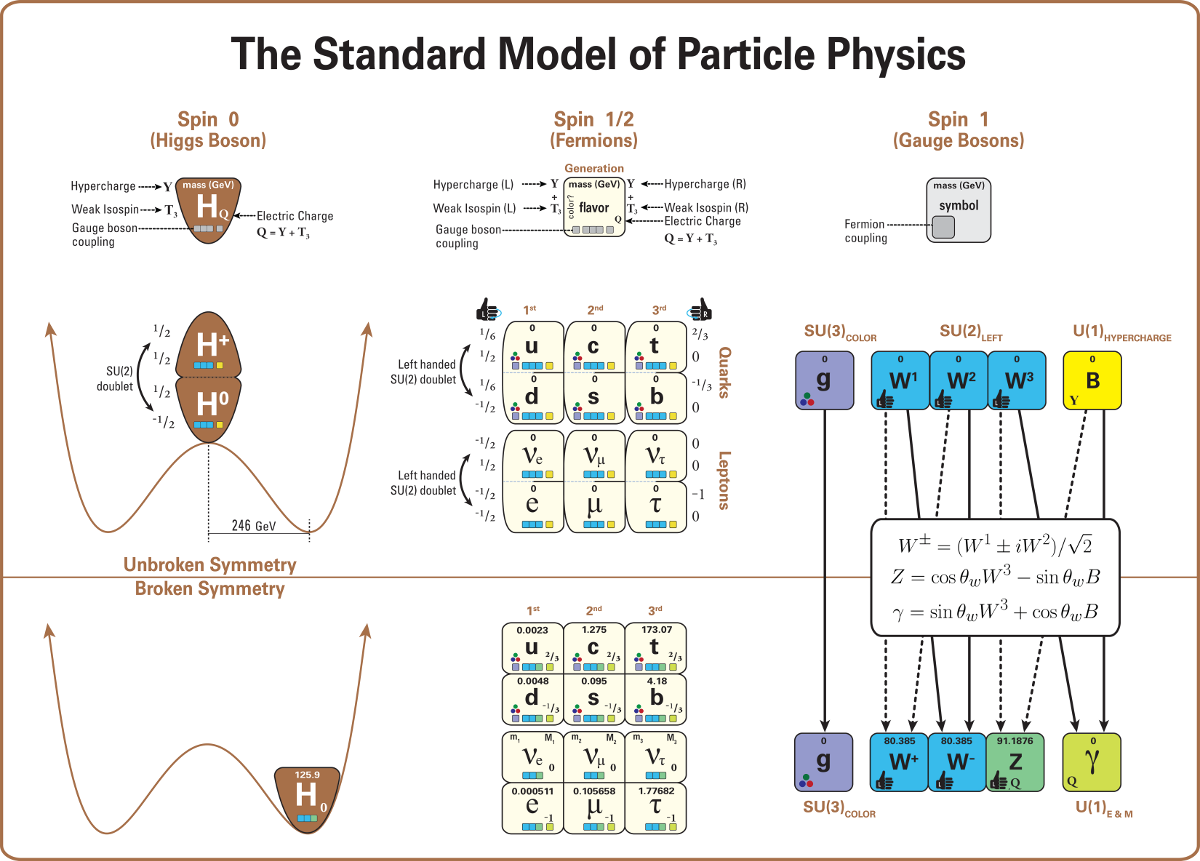
\includegraphics[width=\linewidth]{./figures/standard_model_complete_lowres.png}
	\caption{
		"This diagram displays the structure of the standard model (in a way that
		displays the key relationships and patterns more completely, and less
		misleadingly, than in the more familiar image based on a 4x4 square of
		particles). In particular, this diagram depicts all of the particles in the
		standard model (including their letter names, masses, spins, handedness,
		charges, and interactions with the gauge bosons -- i.e. with the strong and
		electroweak forces). It also depicts the role of the Higgs boson, and the
		structure of electroweak symmetry breaking, indicating how the Higgs vacuum
		expectation value breaks electroweak symmetry, and how the properties of the
		remaining particles change as a consequence."\cite{Boyle2014}.
	}
	\label{fig:standardmodel}
\end{figure}


\clearpage
\section{Modern Deep Inelastic Scattering Experiments}

Here, I hope to highlight the last 40 years or so of physics produced by deep
inelastic scattering experiments. The boundaries of science are pushed by huge
collaborations of men and women working together, starkly contrasting the lonely
pursuits of a handful of scientists in 19th century laboratories.

This era of deep inelastic scattering has unearthed some of the most surprising
and monumental discoveries in physics, from the recent discovery of the
Higgs-particle, to the discovery that protons and neutrons are not fundamental
particles at all, but are instead, highly relativistic balls of gluons.

SLAC Experiments (E80-E155) were some of the first experiments to probe the
proton spin structure, operating from 1978-1999. SLAC pioneered the usage of
spin asymmetries as a means of ruling out models for various parameterizations
of quark structure functions, as well as provided important data constraining
nuclear structure functions. SLAC's experiments focused on understanding the
spin structure of the quarks (but not gluons) within protons.

The European Muon Collaboration at CERN was one of the first major international
efforts to study the underlying structure of protons and neutrons with deep
inelastic scattering. The collaboration produced scientific results from 1979 to
1997. The EMC's major contribution to our understanding of nuclear structure was
to amass evidence which supported the parton model of protons and neutrons, as
well as discovering the self-named `EMC effect', which showed that the volume
`occupied' by quarks scales with heavier nuclei~\cite{Aubert1983}. EMC also
elucidated the effects of quark fragmentation and hadron production, DIS in the
nuclear medium, and produced some of the first measurements of the spin
structure of the proton. Most famously, the EMC originally published the `proton
spin crisis' in its first measurement of the proton spin structure function,
$g1$ where it found the spin carried by the proton's 'valence quarks' is
significantly less than $1/2$~\cite{Ashman1988}. 

CERN produced another collaboration which contributed to our understanding of
nuclear structure, the Spin Muon Collaboration. SMC was active from 1993 to 1998
and used polarized beams of muons to interact with a spin polarized target
(ammonia and later p-butanol). SMC measured virtual photon production
asymmetries, $A_1$, in order to measure information about the proton spin
structure function, $g_1$ (discussed in detail in the following chapter). $g_1$
gives access to the quark polarization of protons. Spin structure physics has
been explored at the COMPASS experiment since 2005. CERN's work to understand
the spin structure of the proton probed the contributions of both the quark, and
gluons. 

The German Electron Synchrotron (DESY) is Germany's the premier accelerator
science laboratory, and has been operating continuously since 1964. DESY's
primary experiments in deep inelastic scattering to understand nuclear structure
have been underway since 1992. DESY operates several deep inelastic scattering
experiments including ZEUS, HERA (H1 and H2) and HERMES.  The scientific goals
of the DESY institute as a whole are broad, since it represents Germany's
premier accelerator physics scientific effort. DESY hosts experiments in
condensed matter physics and astrophysics, addition to its efforts in DIS.
However, the portion of DESY's research program devoted to spin structure seeks
to understand both the quark and gluon contributions to proton spin.

Jefferson Laboratory (JLab) is an electron accelerator complex in Virginia
specializing in the cutting edge of fixed target electron deep inelastic
scattering experiments. Experiments in Hall A, B and C are all involved with
studying both quark and gluon contributions to proton spin.

Finally, there is the Relativistic Heavy Ion Collider, and the experiment
PHENIX. RHIC and PHENIX are discussed in detail in
Chapter~\ref{ch:experimental_apparatus}. This thesis presents an analysis of the
data set recorded in 2013 by the PHENIX detector.

\chapter{Models and Associated Probes For Proton Spin Structure}
\label{ch:modeling_proton_spin}

With the advances made over the last half-century, we have come very close to
obtaining a complete model describing the world around us.  In the realm of
Rapid progress has been made in the last 40 years in the understanding of the
structure of the nucleon. Protons and neutrons make up the majority of the mass
in the visible universe - therefore understanding their nature completely is of
fundamental importance to physics.

In the previous chapter, we discussed in the history behind studying the
structure of matter, leading up to a brief discussion of the contemporary
experiments in proton spin structure. Glaringly, I neglected to discuss the
Relativistic Heavy Ion Collider (RHIC) and the Pioneering High Energy Nuclear
Interaction eXperiment (PHENIX), since I wanted to put the program into a firm
theoretical context in this chapter.

This thesis will discuss the experimental efforts of PHENIX to do something no
other experiment has done - utilize the production of W-Bosons as a direct probe
of proton spin. 

Before we discuss the specifics of this measurement, lets first put proton spin
into a larger context.

\section{Modeling the Proton Structure}

One frequent theme in using particle accelerators to study any kind of nuclear
structure is that we do not ever get to directly look at the innards of a
proton, due to the phenomena of color confinement.

This means that often, we must deal with the process of how partons (quarks,
gluons) fragment and decay after a proton proton collision. Additionally, we
must deal with and account for the scale-variance of the fundamental forces. 

The scale variance of the fundamental forces has large implications for the
strong nuclear force, generally represented by the coupling constant,
$\alpha_S$. This constant scales with distance, and becomes highly
non-perturbative at short distances.

Non perturbative effects are notoriously difficult to include in analytical
models. Additionally, we find that the very structure and distribution of
partons and gluons in the nucleus is a scale-dependent phenomena, that is to
say, if we take measurements at a lower energy, we get a different distribution
of partons and gluons than if we measure at higher energy. This is not to say
that the proton magically changes itself based on energy, but is really more
related to the length scale that we are probing inside of the proton. 

With higher energies, we probe successively shorter length scales. Therefore, to
form a complete picture of proton spin structure, we must probe by scanning over
a broad range of energies (length scales).

Though we generally can analytically deal with writing down models in
perturbative regimes, we cannot simply throw up our hands and give up making
predictions in non-perturbative regimes. To accomplish this, we use a
Factorization Theorem, which provides us a way to mathematically separate an
interaction into perturbative and non-perturbative parts (example,
Figure~\ref{fig:disschematic}). The non-perturbative aspect in the figure (the
X) is often the portion which is experimentally constrained.

\subsection{Structure Functions}

As a note here, for this work on theoretical background of deep inelastic
scattering, I heavily reference Ciprean Gal's clear and coherent introduction to
the subject, published in 2014 (\cite{Gal2014b}), in his thesis describing the
complimentary analysis done at PHENIX at central rapidities.

Given that the proton itself has so far been shown to be a non-perturbative
object, we need a means to model the structure of the interaction when two
protons collide, and generate particles.  Generally, we can calculate a
structure function associated with each hadronic process. The variables we
define to describe the kinematics are (see Figure~\ref{fig:disschematic}):

\begin{gather}
  P \label{eq:P}\\
  Q^2 \equiv -q^2 \label{eq:big_q_sq}\\
    x \equiv { Q^2 \over {2P\cdot q} } \label{eq:x}
\end{gather}

Where $P$  is the total hadron momentum (in our case, the proton's momentum),
$Q^2$ is the energy exchange between the proton and probe lepton, and $x$ is the
fraction of the total proton's momentum carried by the quark scattering with the
lepton. $q$, in Equation~\ref{eq:x} is four-momentum transferred from the lepton
to the quark. 

We can then write down structure functions in terms of these variables. We have:

\begin{gather}
  F_1(x,Q^2) = {1 \over 2}\sum_f e_f^2 \left(q_f(x)+\bar{q}(x)\right)
  \label{eq:f1} \\
  F_2(x,Q^2) = 2xF_1(x,Q^2)\label{eq:f2}
\end{gather}

The subscript, $f$ refers to the quark flavors represented in the structure
functions, with $e_f$ referring to the charge of each quark being summed over
(i.e. ${\pm}{1\over3}$ or ${\pm}{2\over3}$). $q(x)$ refers to the parton
distribution function associated with each quark flavor. 

An integration over the momentum fraction, $x$ of Equation~\ref{eq:f2} and the
gluon structure function $g(x)$ yields the familiar 'valence quark' structure of
the proton, i.e. two up-quarks and one down quark, with remaining quark flavors
$q_h$ summing to zero:

\begin{gather}
	\int_0^1 F_2(x,Q^2) + g(x) dx 
	= \int_0^1 
	\left(
		x\sum_f e_f^2 \left(q_f(x)+\bar{q}(x)\right) 
	\right) 
	+ g(x) dx \label{eq:f2_int_1} \\
	\int_0^1 \left(u(x)+\bar{u}(x) dx \right) dx = 2  \label{eq:up_quark_valence} \\
	\int_0^1 \left(d(x)+\bar{d}(x) dx \right) dx = 1  \label{eq:down_quark_valence} \\
	\int_0^1 \left(q_h(x)+\bar{q}_h(x) dx \right) dx = 0 \label{eq:other_quark_valence}
\end{gather}

The rest of the world data on $F_2(x,Q^2)$ is summarized in
Figure~\ref{fig:f2_world_data}

\begin{figure}
  \centering
  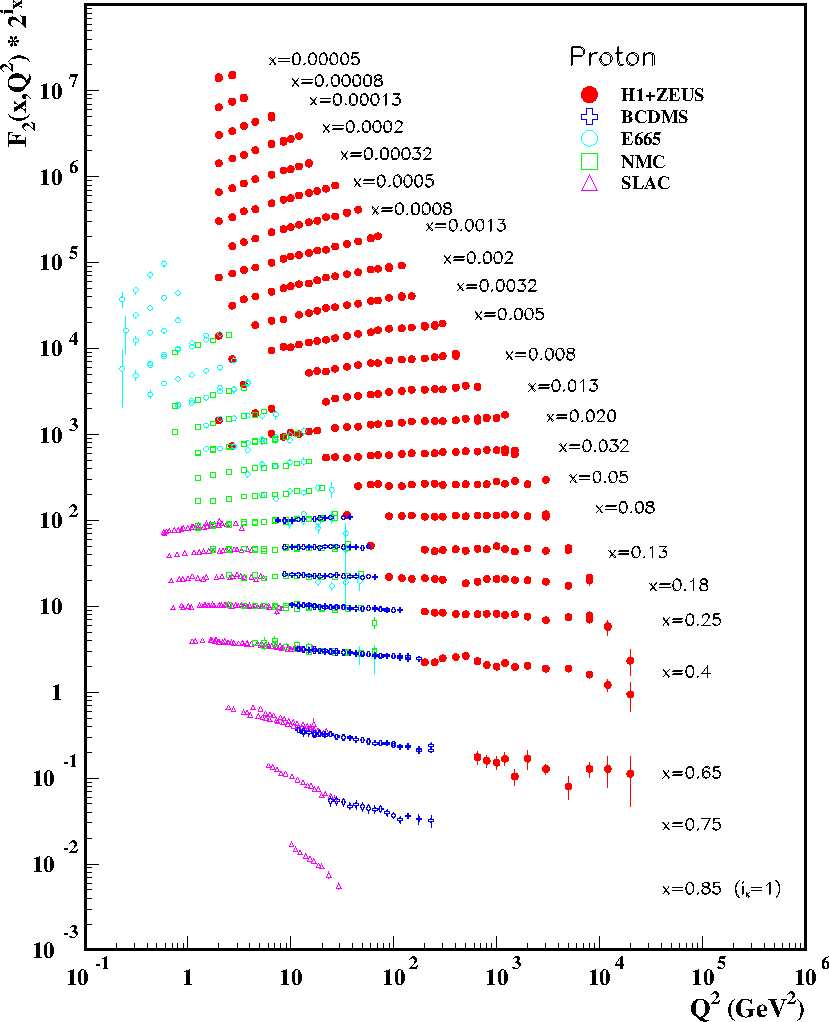
\includegraphics[width=\linewidth]{./figures/F2_structure_function.pdf}
  \caption{
		Here, we see "the proton structure function, $F_2^p$ measured in
		electromagnetic scattering experiments of electrons and positrons on
		protons" from experiments including H1+Zeus, BCDMS, E665, NMC and
		SLAC~\cite{ReviewEidelman2012}
  }
  \label{fig:f2_world_data}
\end{figure}

From this dataset, we can extract Parton Distribution Functions for any
combination of $x$ and $Q^2$. Under this particular framework, we can use the
DGLAP evolution equations to evolve PDFs observed at one $Q^2$ to some other
$Q^2$~\cite{Altarelli2009}. One particular advantage of hadron colliers is to
measure the interactions between gluons and partons between two colliding
partons. 

\section{Parton Distribution Functions}

\begin{figure}[ht]
  \centering
  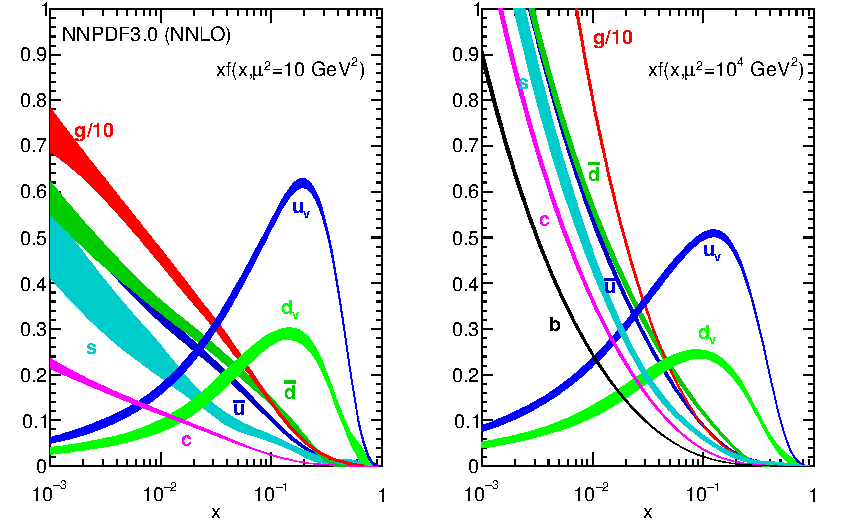
\includegraphics[width=0.7\linewidth]{./figures/unpolarized_pdfs.pdf}
  \caption{
    stuff~\cite{ReviewEidelman2012}
  } 
  \label{fig:unpolarized_pdf}
\end{figure}

\section{Polarized Parton Distribution Functions}
\label{sec:polarized_pdfs}

\begin{figure}
  \centering
  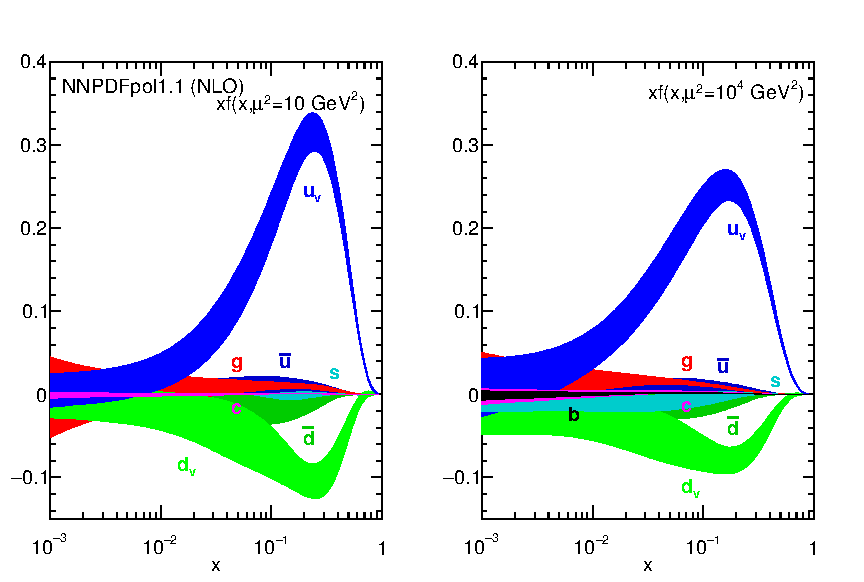
\includegraphics[width=0.7\linewidth]{./figures/polarized_pdfs.pdf}
  \caption{
    stuff~\cite{ReviewEidelman2012}
  }
  \label{fig:polarized_pdfs}
\end{figure}

Discuss DSSV fits
\begin{figure}
  \centering
  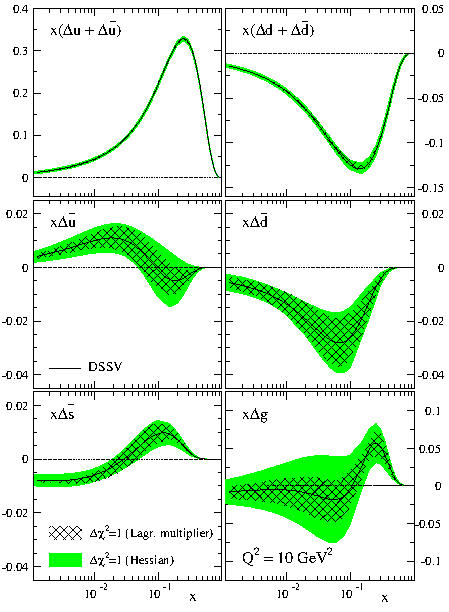
\includegraphics[width=\linewidth]{./figures/polarized_pdfs_dssv.pdf}
  \caption{
    stuff    
  }
  \label{fig:dssv_pdfs}
\end{figure}

\section{Proton Spin Decomposition with the Ellis-Jeffe Sum Rule }

{\noindent}Gauge invariant Ellis-Jeffe
\begin{equation}
  \braket{P,{1\over2}|\hat{J_z}|P,{1\over2}}  
 = {1\over2} = {{1\over2}\Delta \Sigma +L_q+J_g}
\label{eq:ellis_jeffe_sum}
\end{equation}

{\noindent}Infinite momentum decomposition:
\begin{equation}
  \braket{P,{1\over2}|\hat{J_z}|P,{1\over2}}  
  = {1\over2} = {{1\over2}\Delta \Sigma +L_q+\Delta g + L_g}
  \label{eq:infmom_ellis_jeffe_sum}
\end{equation}

{\noindent}Quark decomposition:
\begin{equation}
  {\Delta \Sigma} =
  {
    (\Delta u+\Delta \bar{u})
    +(\Delta d + \Delta \bar{d})
    +(\Delta s + \Delta \bar{s})
  }
  \label{eq:quark_spin_decomposition}
\end{equation}

\section{The Spin Asymmetry: An Experimental Probe }
Write in terms of the cross-section of polarized scattering.

\begin{figure}[ht]
  \centering
  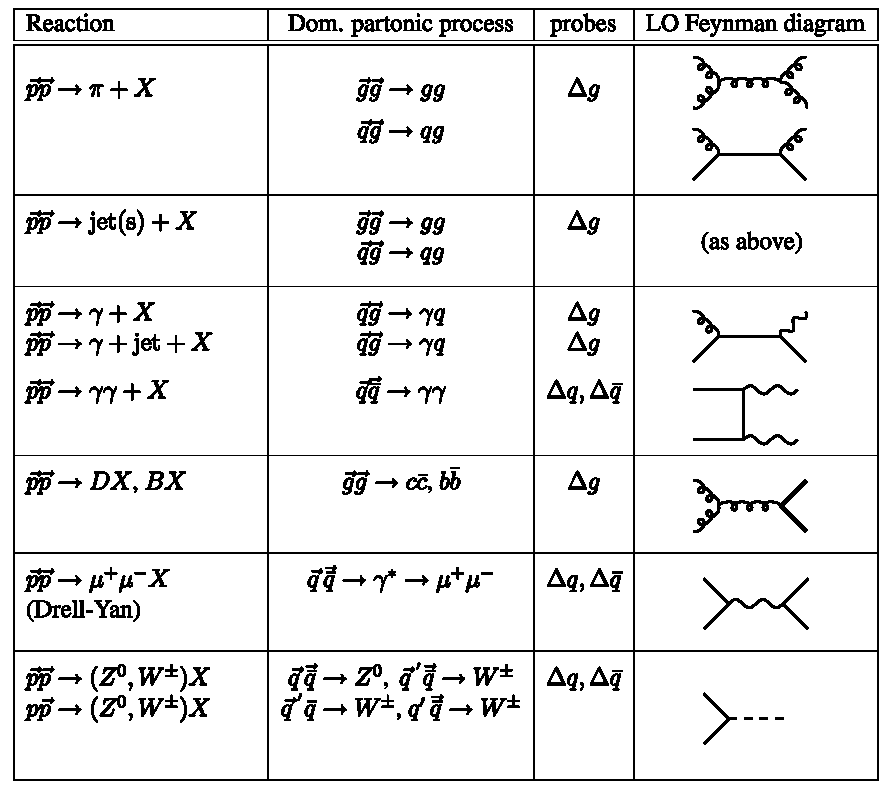
\includegraphics[width=\linewidth]{./figures/spin_probes.pdf}
  \caption{
    A summary of the various probes for longitudinally polarized protons. The
    \textbf{"Reaction"} column summarizes the reaction observed experimentally.
    The \textbf{"Dom. partonic process"} column describes the dominant process
    at the partonic level. The \textbf{"probes"} column shows which proton spin
    structure can be measured with the reaction. Finally, the leading order
    Feynman diagram for the partonic process is drawn. Figure is reproduced
    from: \cite{Aidala2005}.
  }
  \label{fig:spin_probes_masterspin}

\end{figure}

\section{W Production}


Though W-Bosons obviously can be created in collisions with the right
ingredients and correct energy, the W-Bosons that we're interested in at RHIC
are very special. The collision conditions around the protons at colliding at
PHENIX provides just enough energy to create real W-Bosons from interaction of
quarks and anti-quarks between two colliding protons. The energy is not
sufficiently high enough to produce real W-Bosons from other processes in
amounts which would significantly dilute the primary source.

The standard model tells us that W production occurs through a pure vector-axial
interaction, this implies that the helicity of the parents particles - in
particular $u+\bar{d}\rightarrow W^+$ and $\bar{u}+d\rightarrow W^-$ have fixed
helicities, due to the relativistic final state neutrino (which is not measured,
of course). To visualize the leading order of W production, with regards to the
quark-sea element being probed, the leading order diagrams for the interaction
are shown in Figure~\ref{fig:w_probe_leading_order}~\cite{Aidala2005}

Since $\Delta q$, the polarized parton distribution function can be split into
contributions from valence quarks, and also sea quarks, understanding $\Delta
\bar{q}$ is an important step towards understanding $\Delta q$ better to better
understand the total proton spin.

\begin{figure}[ht]
  \centering
  \begin{subfigure}[b]{\textwidth}
    \centering
    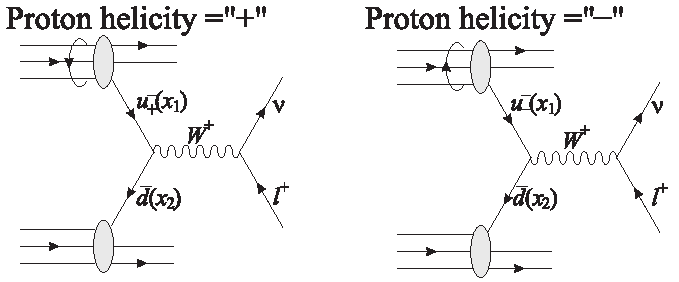
\includegraphics[width=0.8\linewidth]{./figures/w_plus_u_probe.pdf}
    \caption{
      Probe for $\Delta u$ at lowest order.
    }
    \label{fig:u_probe}
  \end{subfigure}
  \begin{subfigure}[t]{\textwidth}
    \centering
    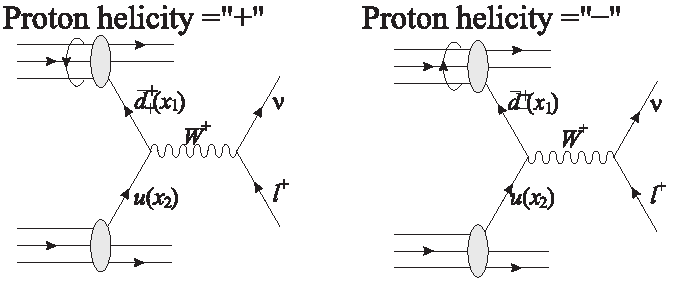
\includegraphics[width=0.8\linewidth]{./figures/w_plus_dbar_probe.pdf}
    \caption{
      Probe for $\Delta\bar{d}$ at lowest order
    }
    \label{fig:dbar_probe}
  \end{subfigure}
  \caption{
    Real $W^+$ production as produced at PHENIX. The helicity of the initial
    state fixes the helicity of the partonic participants due to the
    relativistic final state of the neutrino + the handedness of the W boson.
    $x_1$ and $x_2$ are the momentum fractions of the quarks participating from
    the participant partons~\cite{Aidala2005}. 
  }
  \label{fig:w_probe_leading_order}
\end{figure}

Though both protons in the collision are polarized, the polarization of one
participant proton can be effectively ignored by summing over all polarization
states for one of the two protons. With this assumption, we may construct a
single spin asymmetry for colliding protons by counting difference in the number
of positively and negatively polarized W's produced in collisions, scaled by the
total production:

\begin{equation}
  {{A_L}^W} =
  {{{1}\over{P}}\times{{N_{-}(W)-N_{+}(W)}\over{{N_{-}(W)+N_{+}(W)}}} }
  \label{eq:w_production_asymmetry}
\end{equation}

This is a relatively easy experimental probe to measure (assuming that we can
accurately count events which produced a W, which naturally, is nearly
impossible, as we will see in Section~\ref{sec:sbr}).

As we saw earlier, in Section~\ref{sec:polarized_pdfs}, we can write an
asymmetry in terms of the scattering cross section for the process responsible
for particle yields. These cross-sections were shown to be written in terms of
polarized parton distribution functions, thus, we cut to the chase to write down
the full expression of the theoretical asymmetries for this process in terms of
those parton distribution functions.

The following equations all contain an implied integration over $x_1$ and $x_2$.

For $W^+$ and $u$:
\begin{equation}
  {A_L^{W^+}} = 
  {
    {u_-^-(x_1)\bar{d}(x_2)-u_+^-(x_1)\bar{d}(x_2)}
    \over
    {u_-^-(x_1)\bar{d}(x_2)-u_+^-(x_1)\bar{d}(x_2)}
  }  
  \label{eq:al_u_full}
\end{equation}

For $W^+$ and $\bar{d}$
\begin{equation}
  {A_L^{W^+}} = 
  {
    {\bar{d}_-^+(x_1)u(x_2)-\bar{d}_+^+(x_1)u(x_2)}
    \over
    {\bar{d}_-^+(x_1)u(x_2)+\bar{d}_+^+(x_1)u(x_2)}
  }  
  \label{eq:al_dbar_full}
\end{equation}

Observationally, we see a superposition of \ref{eq:al_u_full} and
\ref{eq:al_dbar_full}, which is expressed in
Equation~\ref{eq:al_superposition_pos}:

\begin{equation}
  {A_L^{W^+}} = 
  {
    {
      \Delta u(x_1)\bar{d}(x_2)-\Delta \bar{d}(x_1)u(x_2)
    }
    \over
    {
      u(x_1)\bar d(x_2)+\bar(d)(x_1)u(x_2)
    }
  }
  \label{eq:al_superposition_pos}
\end{equation}

For the case of $W^-$, we observe $\bar{d}$ and $u$:
For $W^-$ and $d$:
\begin{equation}
  {A_L^{W^+}} = 
  {
    {d_-^-(x_1)\bar{u}(x_2)-d_+^-(x_1)\bar{u}(x_2)}
    \over
    {d_-^-(x_1)\bar{u}(x_2)-d_+^-(x_1)\bar{u}(x_2)}
  }  
  \label{eq:al_d_full}
\end{equation}

For $W^-$ and $\bar{u}$
\begin{equation}
  {A_L^{W^+}} = 
  {
    {\bar{u}_-^+(x_1)d(x_2)-\bar{u}_+^+(x_1)d(x_2)}
    \over
    {\bar{u}_-^+(x_1)d(x_2)+\bar{u}_+^+(x_1)d(x_2)}
  }  
  \label{eq:al_ubar_full}
\end{equation}

Observationally, we see a superposition of \ref{eq:al_d_full} and
\ref{eq:al_ubar_full}, which is expressed in
Equation~\ref{eq:al_superposition_neg}:

\begin{equation}
  {A_L^{W^-}} = 
  {
    {
      \Delta d(x_1)\bar{u}(x_2)-\Delta \bar{u}(x_1)d(x_2)
    }
    \over
    {
      d(x_1)\bar u(x_2)+\bar(u)(x_1)d(x_2)
    }
  }
  \label{eq:al_superposition_neg}
\end{equation}

Kinematics of the collision can simplify the equations even further, when at
very forward or very backward rapidities~\cite{Aidala2005}. Concretely, this is
shown via integration over the momentum fractions, $x_1$ and $x_2$, explicitly
writing the W decay in terms of the scattering cross section for polarized
proton collisions (a derivation reproduced from Hideyuki Oide's
thesis~\cite{Oide2012}):

\begin{multline}
  {
    d\sigma
    \left(
      p^{\Rightarrow}+p\rightarrow W^+\rightarrow \ell+\nu_{\ell}
    \right)
  } 
  = \\
  {
    {K\over3}\int dx_1dx_2\sum_{i,j}
    \left(
    q_{i-}^\Rightarrow(x_1)\bar{q}_{j+}(x_2) +
    \bar{q}_{j+}^\Rightarrow(x_1)q_{i-}(x_2)
    \right)
  }  \\
  \times
  {
    d\hat{\sigma}(q_i+\bar{q}_j\rightarrow W^+\rightarrow \ell^+ + \nu_{\ell})
  }
\end{multline}

{\noindent}Similarly, we may write the interaction cross-section for the
opposite helicity in the initial state:

\begin{multline}
  {
    d\sigma
    \left(
      p^{\Leftarrow}+p\rightarrow W^+\rightarrow \ell+\nu_{\ell}
    \right)
  } 
  = \\
  {
    {K\over3}\int dx_1dx_2\sum_{i,j}
    \left(
    q_{i-}^\Leftarrow(x_1)\bar{q}_{j+}(x_2) +
    \bar{q}_{j+}^\Leftarrow(x_1)q_{i-}(x_2)
    \right)
  }  \\
  \times
  {
    d\hat{\sigma}(q_i+\bar{q}_j\rightarrow W^+\rightarrow \ell^+ + \nu_{\ell})
  }
\end{multline}

Neglecting quark mass, we can assume that the helicity state of the quarks is
identical to the chirality state. Then, we substitute in the definition for
polarized parton distribution functions $\Delta q \equiv q_{+}^{\Rightarrow} -
q_{-}^{\Rightarrow}$, and sum over quark flavors, neglecting strange
contributions:

\begin{align}\label{eq:al_theory_quarks}
  {
    A_L
    \left(
      p^{\Rightarrow}+p\rightarrow W^+ \rightarrow \ell^+ +\nu_{\ell}
    \right)
  } &=  
  {
    {
      \int dx_1 dx_2 \sum_{i,j}
      \left(
        -\Delta q_i(x_1)\bar{q}_j(x_2)
        +\Delta \bar{q}_j(x_1)q_i(x_2)
      \right)\cdot d \hat{\sigma}
    }
    \over
    {
      \int dx_1 dx_2
      \sum_{i,j}(q_i(x_1)\bar{q}_j(x_2)+\bar{q}_j(x_1)q_i(x_2))\cdot d\hat{\sigma}
    }
 }\\
 & \approx  \nonumber
 {
   {
      \int dx_1 dx_2 
      \left(
        -\Delta u(x_1)\bar{d}(x_2)
        +\Delta \bar{d}(x_1)u(x_2)
      \right)\cdot d \hat{\sigma}
   }
   \over
   {
      \int dx_1 dx_2 (u(x_1)\bar{d}(x_2)+\bar{d}_j(x_1)u(x_2))\cdot d\hat{\sigma}
   }
 }
\end{align}

Since we have restricted ourselves to only the case for $u\bar{d}$, we are of
course looking at the case of $A_L^{W+}$. We may rewrite
Equation~\ref{eq:al_theory_quarks} to reflect its rapidity dependance:

\begin{equation}
  {A_L^{W+}(y_{\ell})} = 
  {
    {
     \int dx_1 dx_2 
     \left(
       -\Delta u(x_1)\bar{d}(x_2)(1-cos\hat{\theta})^2
       +\Delta \bar{d}(x_1)u(x_2)(1+cos\hat{\theta})^2
     \right)
    }
    \over
    {
       \int dx_1 dx_2 
       \left(
       (u(x_1)\bar{d}(x_2)   (1-cos\hat{\theta})^2
      +\bar{d}_j(x_1)u(x_2)) (1+cos\hat{\theta})^2
        \right)
    }
  }
  \label{eq:al_w_pos_rapidity_dependance}
\end{equation}

In this case, we follow Dr. Oide's convention of redefining $\hat{\theta}$ in
terms of the angle between the direcion of momentum of the polarized proton and
the leptop in the center of mass frame. Therefore we see kinematic isolation of
the polarized pdfs at forward or backward rapdity.\\

{\noindent}We may write $A_L^{W-}(y_{\ell})$ similarly:

\begin{equation}
  {A_L^{W-}(y_{\ell})} = 
  {
    {
     \int dx_1 dx_2 
     \left(
       -\Delta \bar{u}(x_1)d(x_2)(1-cos\hat{\theta})^2
       +\Delta d(x_1)\bar{u}(x_2)(1+cos\hat{\theta})^2
     \right)
    }
    \over
    {
       \int dx_1 dx_2 
       \left(
         (\bar{u}(x_1)d(x_2)   (1-cos\hat{\theta})^2
         +d_j(x_1)\bar{u}(x_2)) (1+cos\hat{\theta})^2
        \right)
    }
  }
  \label{eq:al_w_neg_rapidity_dependance}
\end{equation}
\clearpage
\section{Cross Sections and Luminosity}
\begin{itemize}
		\item vernier analysis note intro, equations
		\item summarize the papers on Lumoninosity
\end{itemize}

\textbf{Questions I'd Like to Answer in this Chapter}
\begin{enumerate}
    \item Why can we collide two polarized protons, but pretend that only one of
      them is polarized? What if summing over polarization states doesn't
      'cancel' this out?
    \item Why is $A_L$ an appropriate probe for proton spin
    \item How exactly do we go from a measurement of $A_L$ to an understanding
      of proton spin?
    \item Why do we need to calculate $A_{LL}$? What does it tell us? Why do we
      combine the helicities in the way we do, to define $A_{LL}$?
\end{enumerate}

Double spin asymmetry:

\begin{equation}
  A_{LL} = {
    {d\sigma^{\Rightarrow\Rightarrow}-d\sigma^{\Leftarrow\Rightarrow}}
    \over
    {d\sigma^{\Rightarrow\Rightarrow}+d\sigma^{\Leftarrow\Rightarrow}}
  }
\end{equation}
\clearpage

\chapter{The Relativistic Heavy Ion Collider}

\section{Overview}
While there have been many experiments which have performed deep inelastic
scattering over the years, the experiments built around the Relativistic Heavy
Ion Collider at Brookhaven National Laboratory are positioned to take advantage
of this unique accelerator. 

\begin{figure}[ht]
  \centering
  \begin{subfigure}[b]{\textwidth}
    \centering
    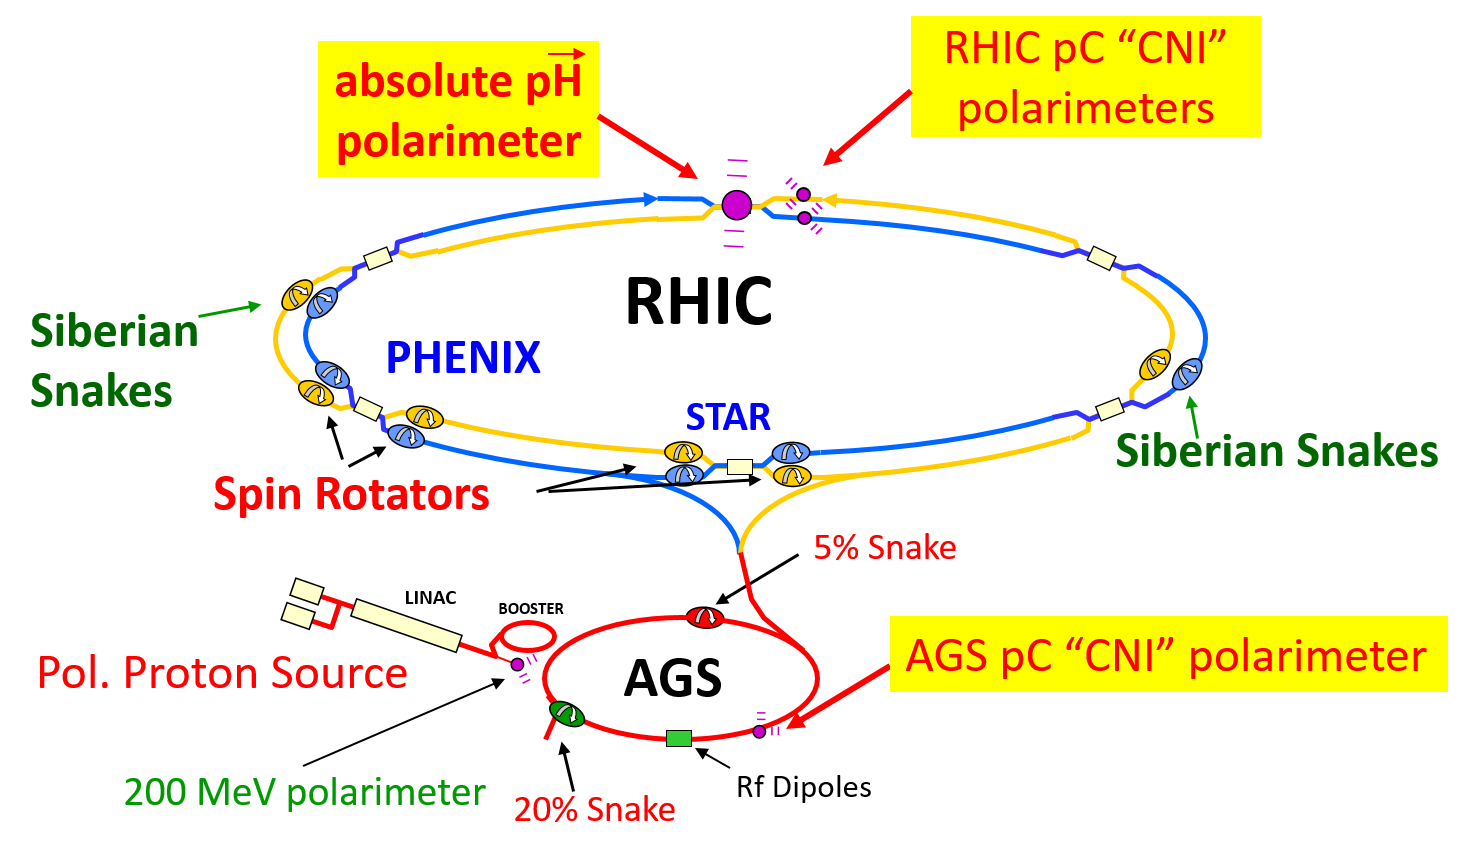
\includegraphics[width=0.8\linewidth]{./figures/kiyoshi_tanida_rhic_schematic.png}
    \caption{Diagram of RHIC Accelerator Complex, (Figure from Kiyoshi Tanida)}
    \label{fig:rhic_schematic} 
  \end{subfigure}
  \begin{subfigure}[b]{\textwidth}
    \centering
    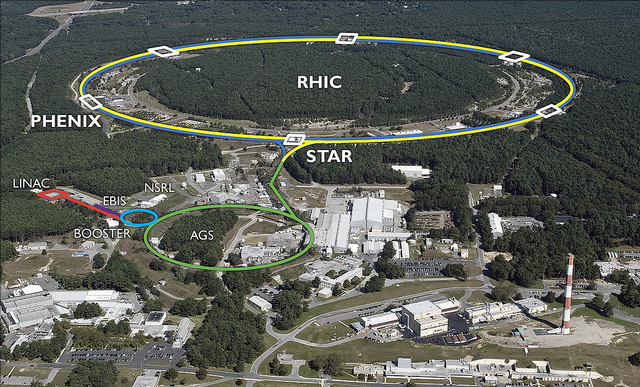
\includegraphics[width=0.8\linewidth]{./figures/7979381212_fddf3f1ab4_z.jpg}
    \caption{Aerial photograph of RHIC Complex \cite{BNLFlickr2011}}
    \label{fig:rhic_aerial}
  \end{subfigure}
  \caption{
		A diagram of the acceleration process of RHIC is shown in the top panel, and
		aerial view is shown in thin the bottom panel. RHIC is nearly four miles in
		circumference and collides a variety of ions at center-of-mass energies
		between $5$ Gev $\sqrt{s}$  and $510$ GeV $\sqrt{s}$.
  }
  \label{fig:rhic_complex}
\end{figure}

The Relativistic Heavy Ion Collider (RHIC) is the world's only intersecting ring
particle accelerator which is capable of colliding polarized proton beams. The
beams are differentiated with the mnemonic ``Blue'' and ``Yellow'' labels. The
blue beam circulates clockwise when viewed from above the RHIC complex, the
yellow beam circulates counter-clockwise. As is typical for intersecting ring
experiments, the beams are bunched, with bunches of ions intersecting at
designated intersection points, around which experiments are built.  The filled
bunches from the blue and yellow beams cross at a frequency of 106 nanoseconds.
PHENIX's timing is set to correspond to the crossing rate of the blue and yellow
beams. Because bunches always collide simultaneously, the blue beam timing clock
is used as a matter of convention, though there are other timing clocks
available for use. The bunches in the beams are numbered as a means of
associating the bunch polarization configuration with the bunch crossing at each
interaction region. This is necessary for any measurement which requires a
knowledge of the initial polarization state of colliding hadrons (such as any
spin physics measurement). This will be discussed more in the section of
discussing the beam polarization at RHIC~\ref{sec:beam_polarization}.

RHIC generally separates data taking into beam `fills' which are uniquely
numbered, and for which general data characterizing the machine state is logged
in various databases and online logbooks. Logging is an important part of data
quality assurance, but also plays a fundamental role in the physics. For
example, the initial spin state of the colliding bunches is logged in databases,
without which, spin analyses are impossible. The trigger configuration is
recorded along with the rates associated with each trigger. Data logged into
logbooks and databases characterizing a fill's performance also plays an
important forensic role with regards to solving issues which occurred during
data taking, but were not immediately caught. Furthermore, because PHENIX is an
international collaboration, this logged data is fundamentally important to
communicating the state of the machine and data collection to the collaboration,
as well as establishing a record of operations.  

RHIC fills are composed of a unique population of bunched ions, circulating
around the rings. During polarized fills, every bunch is polarized according to
a planned polarization pattern. At the end of each fill, (typically 8 hours of
collisions), the beam is dumped, and a new fill is generated.  Experiments built
around RHIC generally subdivide fills into `runs', where a run is a period of
time where the experiment is taking data during which there were no obvious
machine malfunctions. When major issues occur during a run, data taking is
interrupted until the problem is remedied, and the data is discarded. At PHENIX,
runs are always segregated within a fill--no run will ever contain data from
multiple fills, due to the additional complexity of potentially changing machine
conditions, significant down-time between fills, and the potential of beam-dumps
into sensitive high voltage enabled electronics.

Scientists at RHIC have come up with many ingenious ways to create and maintain
beam polarization (Section~\ref{sec:beam_polarization}), once this is
accomplished, various kinematically select probes are engineered, based on
collisions observed which provide important cross-checks to DIS data as well as
original discoveries and measurements of proton structure. RHIC is a unique
collider in that it is quite flexible. Beams may be transversely or
longitudinally polarized, a variety of ions may be used to fill the beams. To
date, RHIC has collided many beam ions and species, summarized in
Figure~\ref{fig:rhic_early_run_summary} and
Figure~\ref{fig:rhic_late_run_summary}.

RHIC is an facility which has been built on top of previous accelerator
experiments--a Linear Accelerator, a booster ring, and an Alternating Gradient
Synchrotron, all of which now have been re-purposed to create the necessary beam
injection conditions appropriate for RHIC. Many experiments are still set up
around various egress points along the acceleration chain, which are publicised
on the Brookhaven National Laboratory website \url{www.bnl.gov}

\begin{figure}[ht]
  \centering
  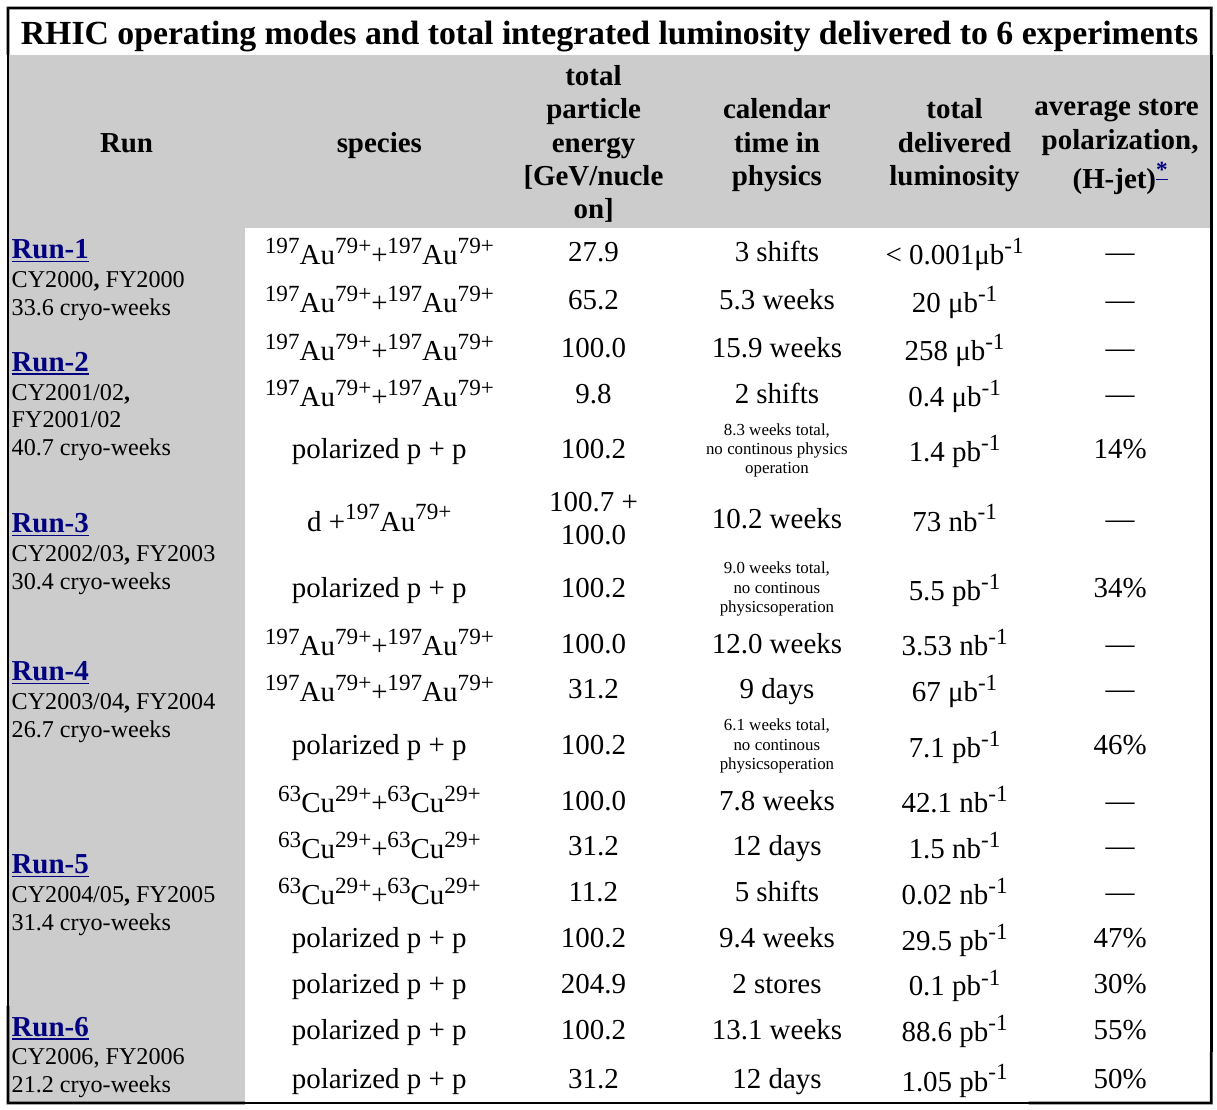
\includegraphics[width=0.8\linewidth]{./figures/rhic_early_run_summary.png}
  \caption{ 
    Runs 1--3 at RHIC focused on commissioning work for experiments measuring
    collisions at RHIC. Work was mostly characterized by heavy-ion measurements
    related to understanding Quark-Gluon Plasma. The spin program began with Run
    5. Table produced from data posted at the RHIC run page \cite{Fischer2016}.
  }
  \label{fig:rhic_early_run_summary}
\end{figure}

\begin{figure}[ht]
  \centering
  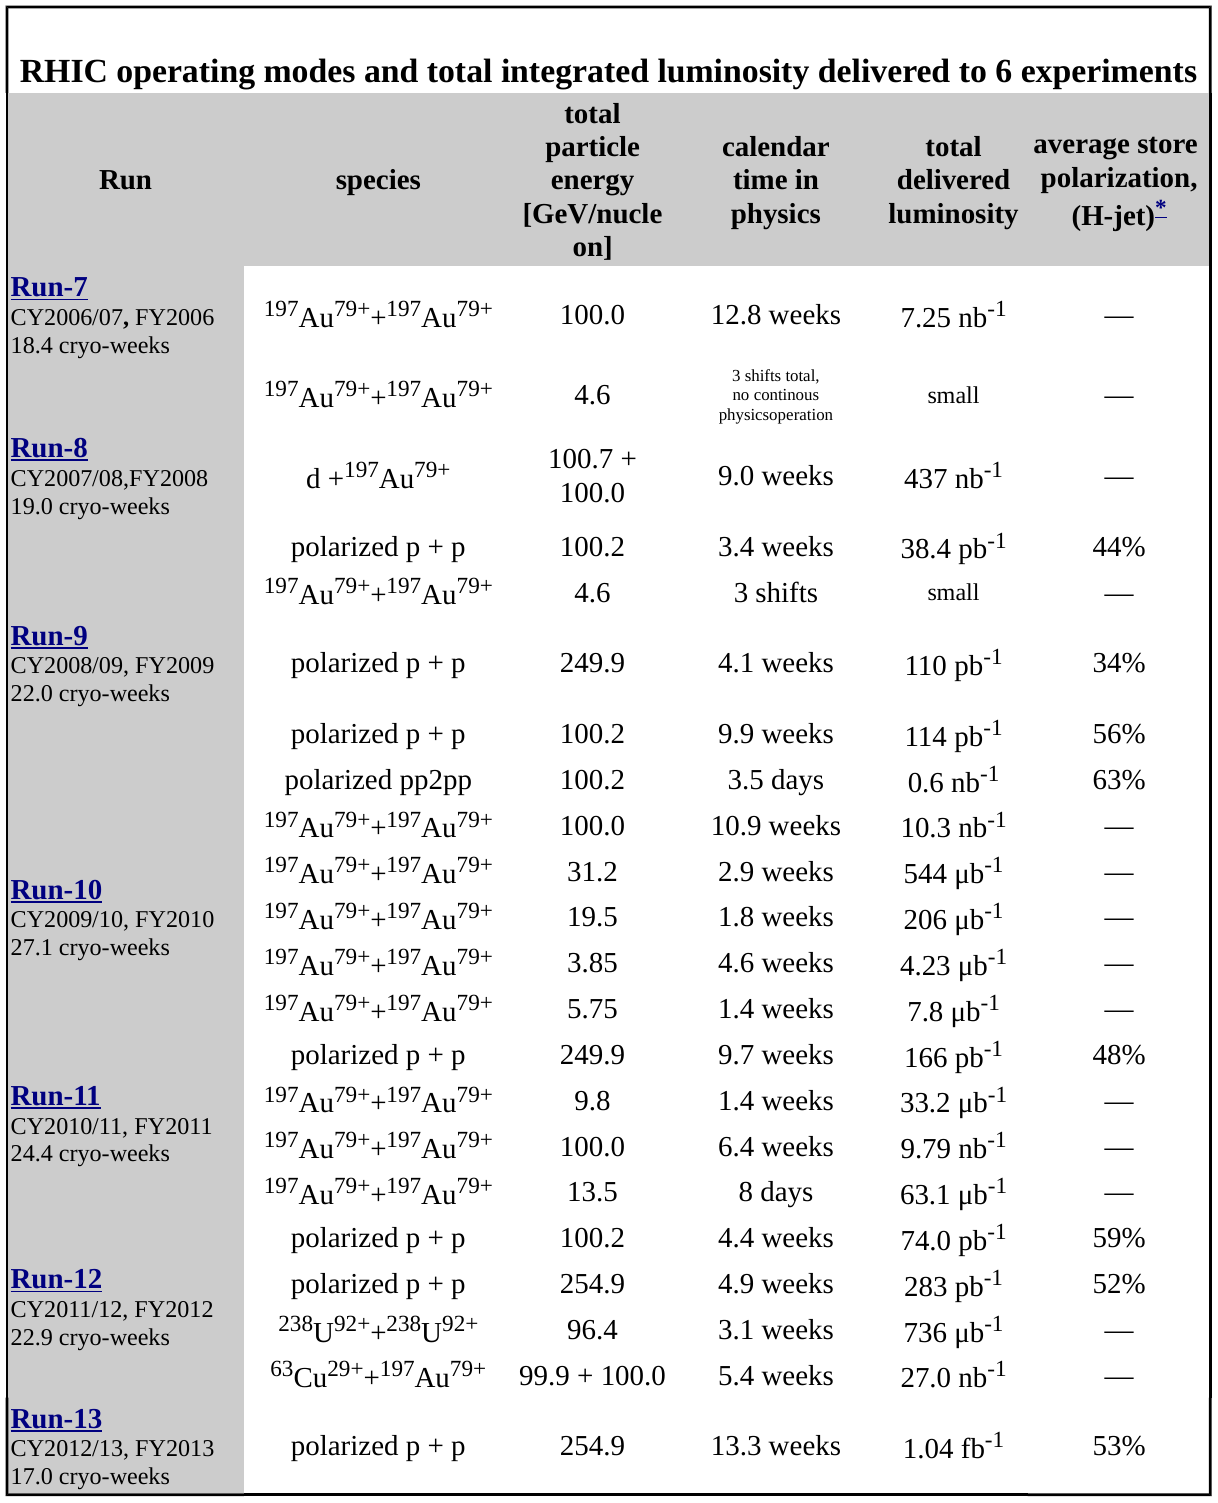
\includegraphics[width=0.8\linewidth]{./figures/rhic_late_run_summary.png}
  \caption{ 
    Though RHIC is currently still running (as of May 9, 2016), I include runs
    here up to and including the run producing my data set (Run 13). An
    unprecedented 13.3 cryo-weeks of running was awarded to the W-Physics
    group.  Table produced from data posted at the RHIC run
    page \cite{Fischer2016}.
  }
  \label{fig:rhic_late_run_summary}
\end{figure}

At the time of writing of this Thesis (Spring of 2016), there are two
experiments which are actively taking data from collisions produced by RHIC: The
Pioneering High Energy Nuclear Interaction Experiment (PHENIX,
Section~\ref{sec:PHENIX}, Figure~\ref{fig:phenix_and_star}), and the Solenoidal
Tracker at RHIC (STAR, Figure~\ref{fig:phenix_and_star}). STAR and PHENIX are
complimentary to each other--PHENIX has a very high precision centrally covering
Electromagnetic Calorimeter, and other high precision detectors, but lacks full
kinematic coverage, whereas STAR has lower precision (with some measurement
dependent exceptions), but has the advantage of nearly full kinematic coverage
around the beam intersection at its center.

RHIC's luminosity and beam polarization has been continuously improving
(Figure~\ref{fig:rhic_luminosity}) since RHIC was first turned on. As we will
discuss later (Section~\ref{sec:forward_upgrade}), the increased luminosity
observed in 2013, was maximally leveraged with upgrades to the PHENIX detector.

\begin{figure}[ht]
  \centering
  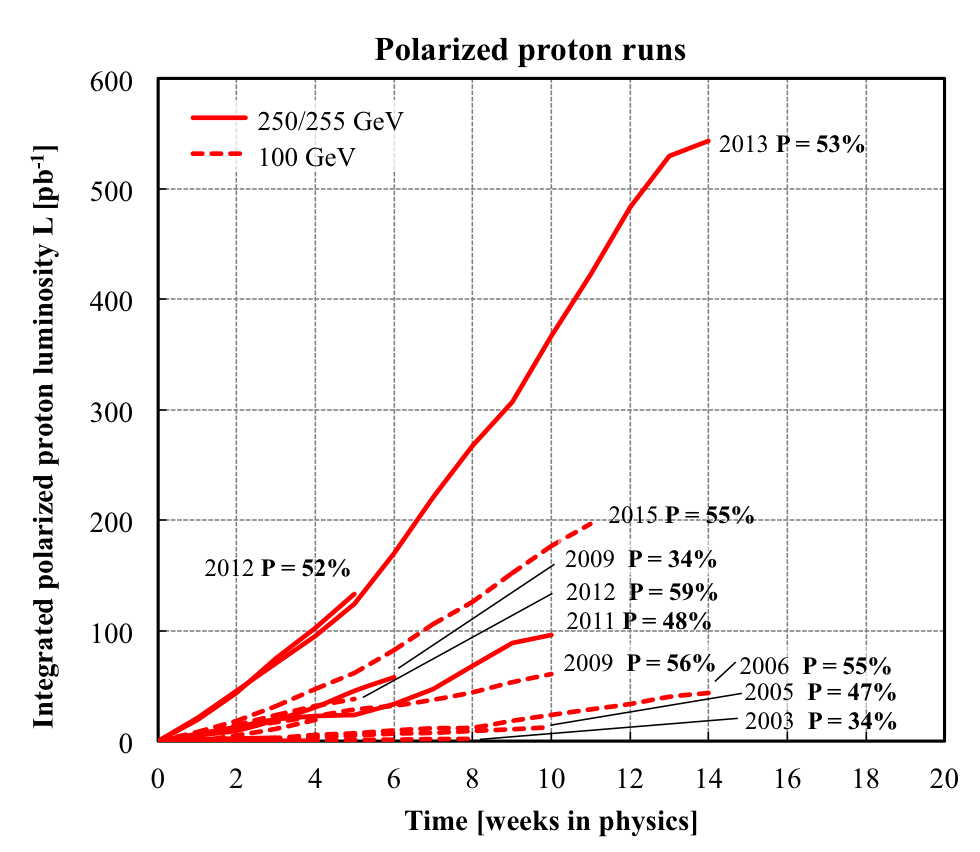
\includegraphics[width=0.8\linewidth]{./figures/RhicLuminosityPP.png}
  \caption{
    Upgrades to RHIC's electron lens have enabled massive improvements to
    luminosity--seen in the year 2013. The high luminosity was taken advantage
    of with an extra long proton+proton run. Figure obtained from
     \cite{Fischer2016}
  }
  \label{fig:rhic_luminosity}
\end{figure}


\clearpage

\subsection{Experimental Apparatus}

\begin{figure}[ht]
  \centering
  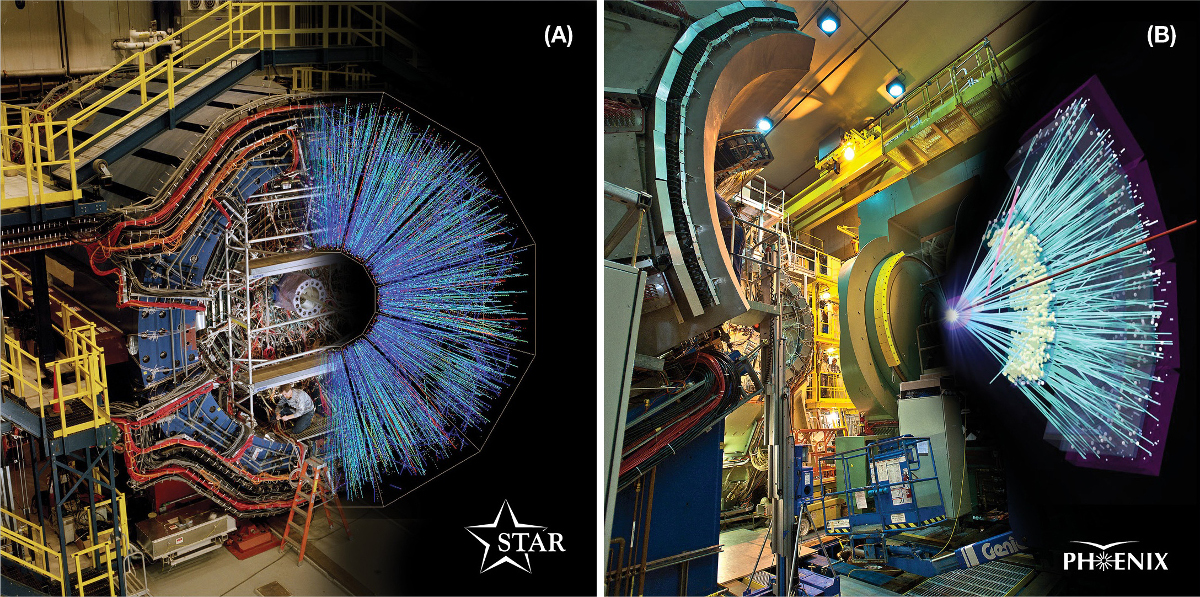
\includegraphics[width=\linewidth]{./figures/rhic_graphics_fig2-hr.jpg}
  \caption{
    STAR (a) and PHENIX (b) with cutaways showing the event display for a
    heavy-ion collision as reconstructed by the detectors' electromagnetic
    calorimeters~\cite{Walsh2012}.
  }
  \label{fig:phenix_and_star}
\end{figure}

RHIC accelerates ions in a multi-stage process, summarized in
Figure~\ref{fig:rhic_complex}. The source of the beams is the \textbf{Electron
Beam Ion Source}, built on top of a $200$ MeV linear accelerator (Linac). Once
ions are injected into the Linac, they travel to the \textbf{Booster
Synchrotron}.  At this stage, ions are accelerated with pulsed RF fields. After
the beam of ions has been accelerated to nearly the speed of light, they are fed
into the \textbf{Alternating Gradient Synchrotron} or AGS. At this time, ions
are traveling at about 0.37~$c$. By the time the ions leave the AGS, they are
moving at 0.997~$c$. When the ions have reached the appropriate injection energy
(which is ion-species dependent), they are transferred to the
\textbf{AGS-to-RHIC Line}, where a switching magnet pumps bunches of ions into
either the counterclockwise circulating ring of RHIC, or the clockwise
circulating ring of RHIC. The ions are accelerated here to maximum speed--each
beam-ion travels a distance of 2.4 miles every 12.8 microseconds (0.99999~$c$ at
510 GeV $\sqrt{s}$ beam energy), for the duration of a
physics-fill~\cite{RHIC2016}.

When the RHIC rings are filled with ions, the ions are bunched into rotating
electromagnetic potentials called `buckets'. There are 360 beam-buckets in
total, but typically only a fraction are filled with ions. For this analysis, we
took data with beams with 110 filled buckets. The sequence of beam buckets from
one filled bunch to the next is referred to as a `bunch'--and are rather long -
Figure~\ref{fig:bunch_profile_overlay}. The bunch length is 12 meters
longitudinally. The bunch width is quite narrow--with Gaussian geometry, it is
between 150 mm and 300 mm depending on the beam energy.  Understanding the beam
bunch geometry is a crucial component to understanding total the total
luminosity delivered by RHIC to PHENIX. . A detailed presentation of beam
dynamics with regards to luminosity will be presented in chapter
\ref{ch:vernier_analysis}. 

\begin{figure}
  \centering
  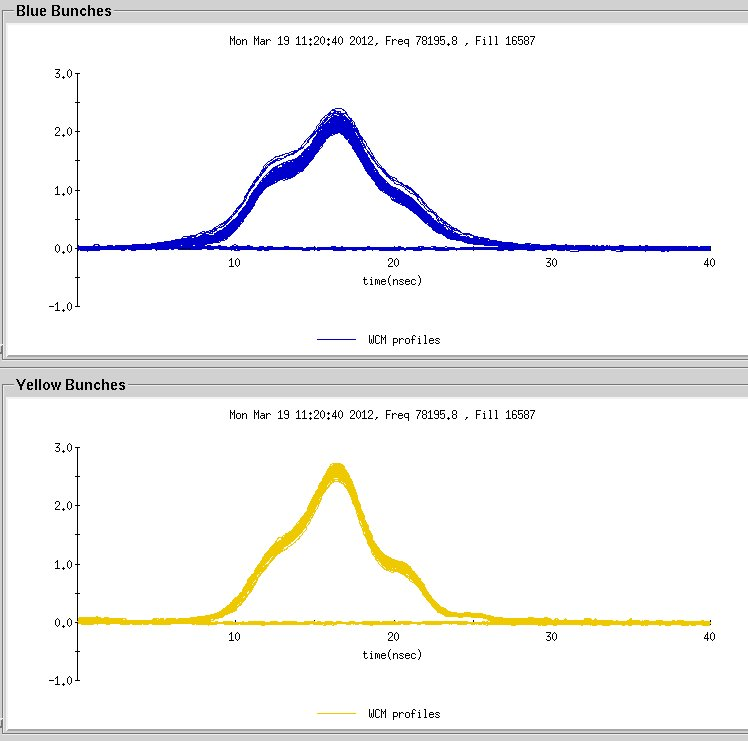
\includegraphics[width=0.7\linewidth]{./figures/wcm_16587.jpeg}
  \caption{
		The longitudinal distribution of all bunches in a typical fill are overlaid.
		The bunches from the blue beam (top) and yellow beam (bottom) are shown for
		over a 40 nanosecond time period. 
  }
  \label{fig:bunch_profile_overlay}
\end{figure}

\clearpage
\section{Production of Polarized Proton Beams}

\textbf{\textcolor{red}{Resume Here!}}

The production of polarized beams is crucial to the physics of this measurement
- without polarized beams, no spin structure analysis can be done at RHIC. This
is due to the fact that the helicity state of the protons in the initial state
of any proton proton collision can be connected to the final observed states in
a way which provides information about the spin structure function, as was
discussed in section \ref{ch:modeling_proton_spin}. 

The production of polarized beams is a multistage process, and involves several
experimental components. The importance of polarizing the beams is fully
realized once polarized beams are collided at relatively high center of mass
energies--where the beams behave less like polarized proton beams, but more
like polarized beams of quarks and gluons \cite{Alekseev2003}.  Beam
polarization is achieved incrementally--with polarization starting as soon as
the booster and AGS stage of the acceleration process \ref{fig:rhic_complex}.

The RHIC Configuration Manual \cite{RHIC2006} provides a wealth of information,
accelerator physics, diagrams, equations, and descriptions of the extremely
precise and comprehensive approach to creating polarized proton beams and
injecting them into RHIC. This work was crucial to this section of my thesis,
and is recommended reading for anyone who wishes to know `all the details' of
how RHIC handles polarized beams.

\subsection{Polarized Injection}

RHIC uses an optically pumped polarized ion source (OPPIS),
Figure~\ref{fig:rhic_oppis} to produce a polarized ion source greatly in excess
of RHIC's design intensity. This is used to our advantage, as the emittance of
the beam can be lowered to create a highly collimated beam for physics use.

\begin{figure}[ht]
	\centering
	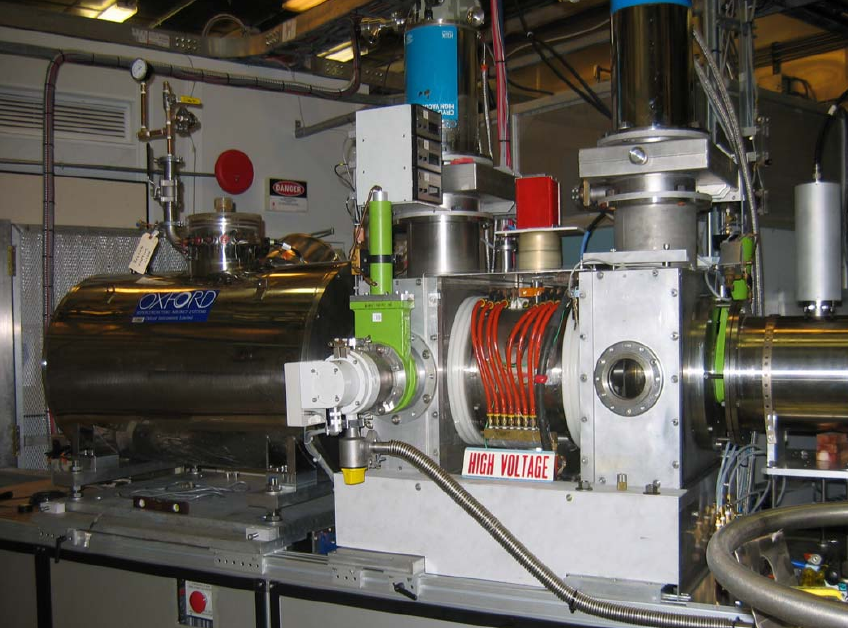
\includegraphics[width=0.8\linewidth]{./figures/rhic_oppis.png}
	\caption{
		RHIC's optically pumped polarized ion source. Produces 0.5-1.0 mA current of
		polarized $H^-$ ions. The optical pumping is pulsed at 400
		$\mu$s, \cite{Zelenski2007}
	}
	\label{fig:rhic_oppis}
\end{figure}

\clearpage
\subsection{AGS to RHIC Transfer Line}

\begin{figure}
  \centering
  \begin{subfigure}[b]{\textwidth}
    \centering
    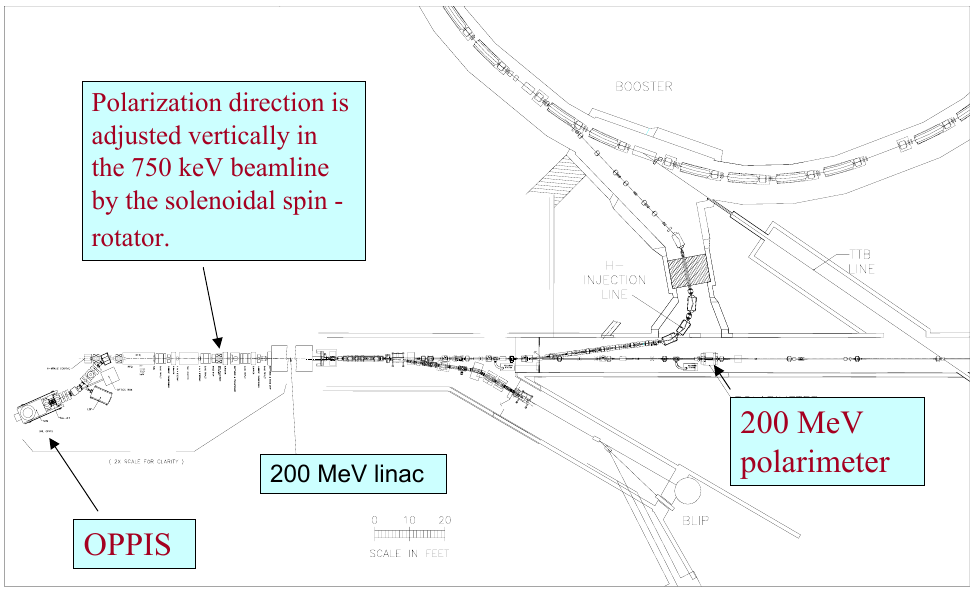
\includegraphics[width=0.7\linewidth]{./figures/rhic_polarized_injector.png}
		\caption{
			Technical schematic of Polarized Injection Line \cite{Zelenski2007}
		}
    \label{fig:polarized_top_view_1} 
  \end{subfigure}
  \begin{subfigure}[b]{\textwidth}
    \centering
    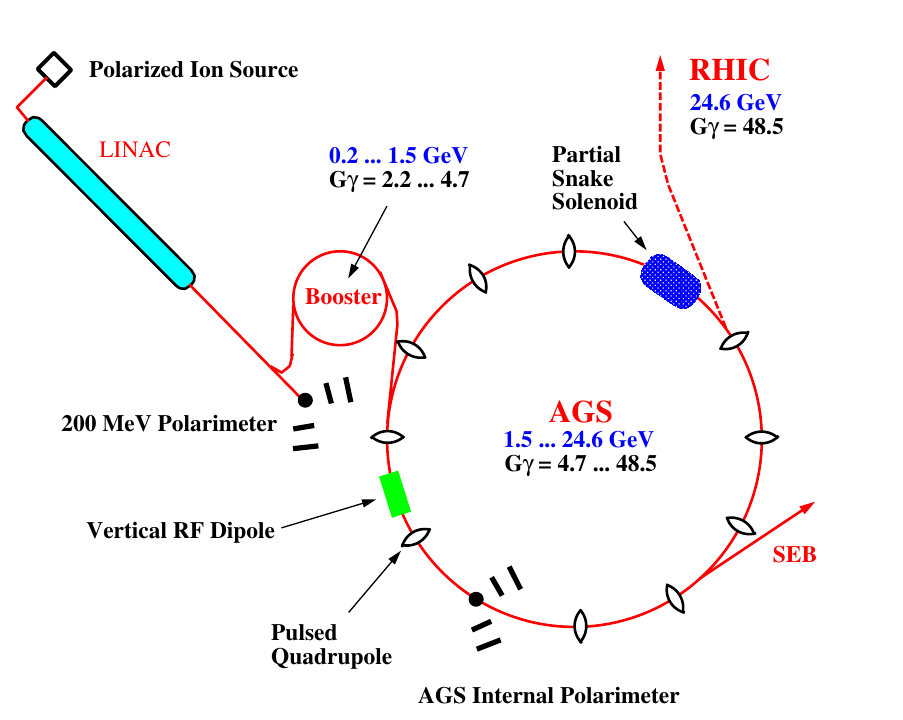
\includegraphics[width=0.7\linewidth]{./figures/polarized_beam_rhic_complex.png}
		\caption{
			Overhead view of Polarized Injection Line \cite{RHIC2006}
		}
    \label{fig:polarized_top_view_2}
  \end{subfigure}
  \caption{
		A view of the RHIC polarized injection system. We see a zoomed in technical
		view of the OPPIS to the booster (a), below, we see a zoomed out cartoon of
		the next step in the polarization injection system, including the AGS, and
		the feeder line to RHIC.
  }
  \label{fig:rhic_polarized_beam_line}
\end{figure}

Once ions have been optically pumped, we have a direct-current beam at
approximately 80\% polarization. The pumping is accomplished using Rubidium
vapor. The polarized ions are then moved into the booster from the Linac, where
some polarization is lost to spin precession, intrinsic to accelerating charged
ions in a circular path. However, polarization is maintained, for the most part,
by matching the precession resonance to the orbiting frequency of the booster
ring. The Siberian snakes and spin rotators at this stage serve to incrementally
flip the ion spin such that the natural depolarization works to re-polarize the
orbiting ions, every full-turn. The full details of this procedure are well
described in \cite{RHIC2006}.

After the ions are sufficiently polarized and filled in the AGS, they are moved
into the AGS to RHIC Transfer line, Figure~\ref{fig:ags_to_rhic}. The beam is
focused and fed through a switching magnet--which must be timed with great
precision in order to fill the blue and yellow beams with the appropriate
polarization patters. In fact, the precision is so great, that the earth's
curvature must be taken into account over this relatively short injection line -
the entry point and exit point are bent ever slow slightly different--the entry
being 12.51 mrad, vs the egress being 12.46 mrad \cite{RHIC2006}. At the point
of injection in the transfer line, the beam size and emittance are measured, as
well as the beam polarization. 

\begin{figure}
  \centering
  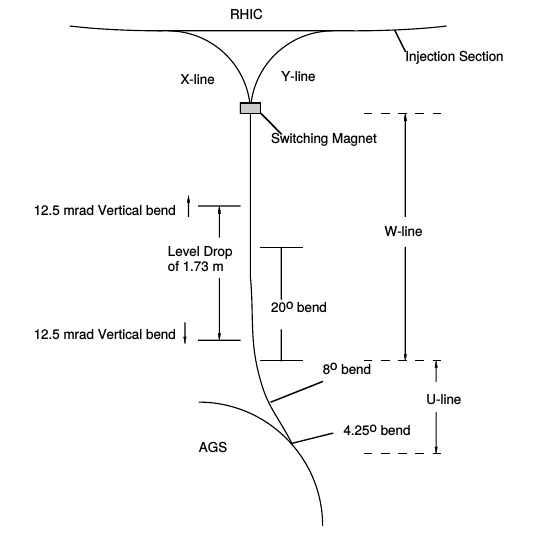
\includegraphics[width=0.6\linewidth]{./figures/ags_to_rhic_transfer}
  \caption{
    A schematic of the geometry of the AGS-to-RHIC transfer line~\cite{RHIC2006}.
  }
  \label{fig:ags_to_rhic}
\end{figure}

\clearpage
\section{Maintaining Beam Polarization}
\label{sec:beam_polarization}

The creation of polarized beams is only half the battle. Depolarizing resonances
in any particle beam are intrinsic in the design of any circulating beam
particle accelerator--without intervention, after a few rotations, RHIC's
polarized beams would be unpolarized. RHIC uses several strategies in concert to
correct for the largest of these depolarizing resonances--including beam orbit
corrections, the Siberian Snakes, Betatron Tune Spreading, and sextupole
magnetic depolarizing resonances. 

\subsection{Siberian Snakes and Spin Rotators}

The Siberian Snakes are positioned at two locations on the RHIC ring (as well as
others along the injection sequence). The most stable configuration of spin
injected in RHIC is such that the spin axis is perpendicular to the plane of the
accelerator ring. The Siberian snake is a helical magnet which forces the spin
to rotate 180 degrees every half rotation. This special configuration of snakes
(see Figure~\ref{fig:rhic_complex}) ingeniously takes advantage of the
rotational precision of the spin (a depolarizing resonance) to re-polarize the
beam, every half-orbit.

The spin rotators are located outside of experimental interaction regions around
PHENIX and STAR. These special dipole magnets rotate the spin of the beams onto
a longitudinal (parallel with beam) axis--these magnets are important for any
measurement (such as this one) requiring longitudinal spin polarization.
Otherwise, transverse spin effects can by studied.

\subsection{Measuring Beam Polarization}

The RHIC Collider-Accelerator Department provides several means of measuring the
beam polarization over the course of the data taking period. PHENIX takes
special data and studies it, to determine the real beam polarization delivered
to the detector, in a yearly analysis (for years where polarized data is taken).
This analysis is often called ``Local Polarimetry'', but is often abbreviated as
LPol in PHENIX logs.

CAD will additionally measure polarization in via inelastic proton-carbon
scattering in the Coulomb-Nuclear Interference (CNI) region. Relative
polarization can be determined with to within 10\% in only a few seconds of
measurement. 

Vertical polarization is determined through the calculation of the left and
right particle production, with a known analyzing power (\cite{RHIC2006}, Ch 8):

\begin{equation}
  P_B = {{1}\over{A_p}}{{N_L-N_R}\over{N_L+N_R}}
  \label{eq:rhic_polarization}
\end{equation}

Where $P_B$ is the beam polarization, $N_L$ and $N_R$ are the left-scattering
produced particles, and right-scattering produced particles and $A_p$ is the
analyzing power, which can be calculated from first principals, and
experimentally verified. Scattering takes place as a carbon filament is swept
across the beam.

As many decisions are financially constrained, this one was too. Using a
p-Carbon CNI polarimeter provides an economically viable way to measure beam
polarization within the precision needed for the spin experiments.

\subsubsection{The Spin Monitor}
\label{sec:the_spin_monitor}

One of my major contributions to the PHENIX experiment was in the upkeep and
development of the spin monitoring systems for the online data taking portions
of the experiment.

During a RHIC run, it is crucial to keep track of the polarization patterns
being collided at the PHENIX IR~\ref{fig:phenix_spin_collision}

\begin{figure}
  \centering
  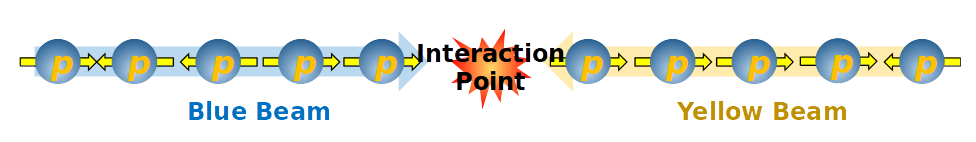
\includegraphics[width=\linewidth]{./figures/phenix_spin_collision}
  \caption{
    As beams are longitudinally rotated into position for collision, it is
    crucial to keep careful track of the magnet currents rotating the beams, as
    well as the overall polarization pattern. Shown is a carton of one potential
    polarization pattern.
  }
  \label{fig:phenix_spin_collision}
\end{figure}

The spin monitor was composed of tens of thousands of lines of code, and was
quite a monstrosity to keep running, however, I managed it. I contributed better
error logging, and helped to facilitate a total rewrite of the software, to
create more understandable and reliable output. However, in the interim, I
reprogrammed the monitor to handle spin patterns, and provide the shift crew at
PHENIX with immediate feedback regarding the spin-quality of the live data,
Figure~\ref{fig:spin_monitor}

\begin{figure}
  \centering
  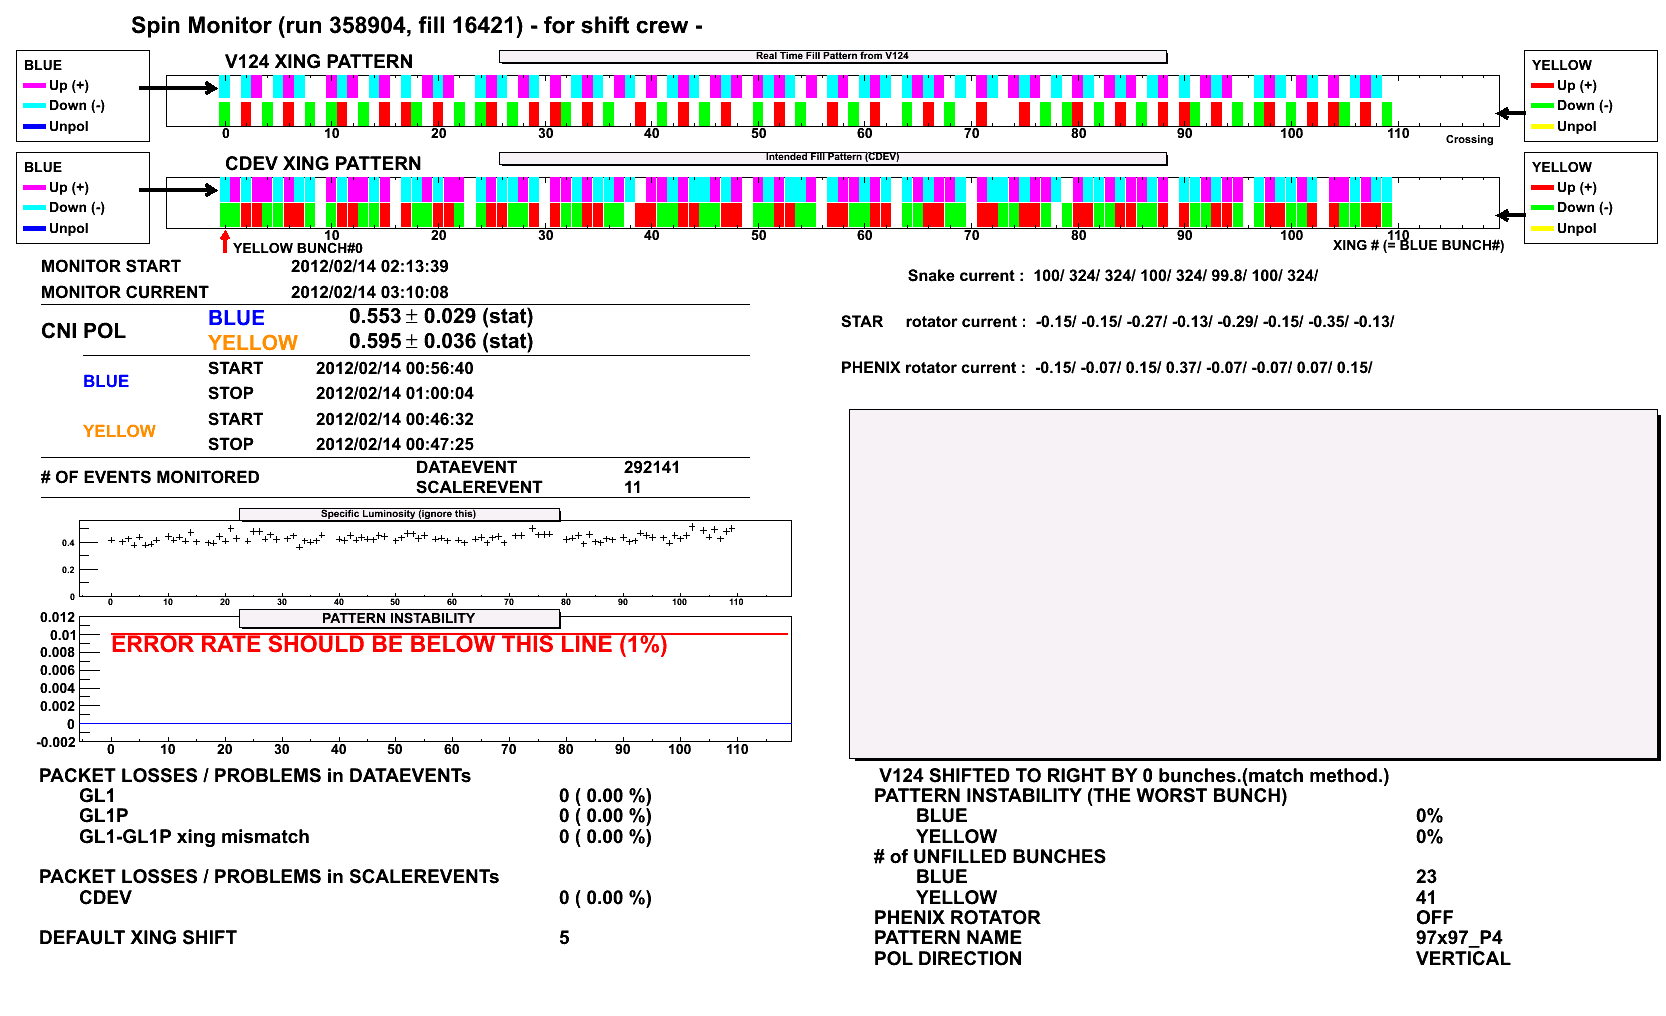
\includegraphics[width=\linewidth]{./figures/SPINMON_shift_358904.png}
  \caption{
    The shift-crew display output for the Spin Monitor. The upper panel shows
    the polarization of the blue and yellow beams, and other panels summarize
    information including magnet currents (needed to understand the spin
    orientation), issues with data packet loss, the recognized spin-pattern, as
    well as a large boxed area on the lower left where errors could be shown to
    the shift crew along with the proper response.
  }
  \label{fig:spin_monitor}

\end{figure}


\clearpage
\section{The Pioneering High Energy Nuclear Interaction Experiment}
\label{sec:PHENIX}
The Pioneering High Energy Nuclear Interaction Experiment is a synthesis of many
smaller detectors all of whom were commissioned for various physics goals, some
of which have been repurposeed from their original application once the primary
physics mission of the detectors were completed.

The configuration of the PHENIX spectrometer can be changed from year to year,
depending on the analysis needs of the physics working groups. The configuration
of the detector for the 2013 physics run is shown in
Figure~\ref{fig:phenix_2013_config}.

\begin{figure}
  \centering
  \begin{subfigure}[t]{\textwidth}
    \centering
    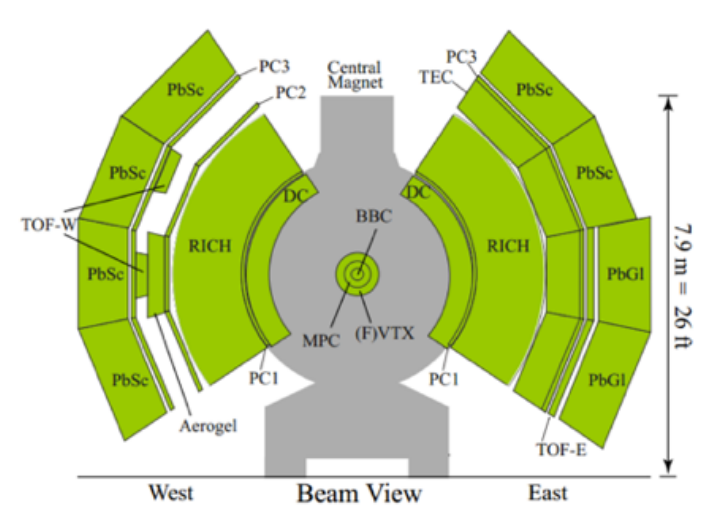
\includegraphics[width=0.8\linewidth]{./figures/phenix_2013_config_central_arms}
    \caption{Central Arms}
    \label{fig:phenix_central} 
  \end{subfigure} 
  \begin{subfigure}[t]{\textwidth}
    \centering
    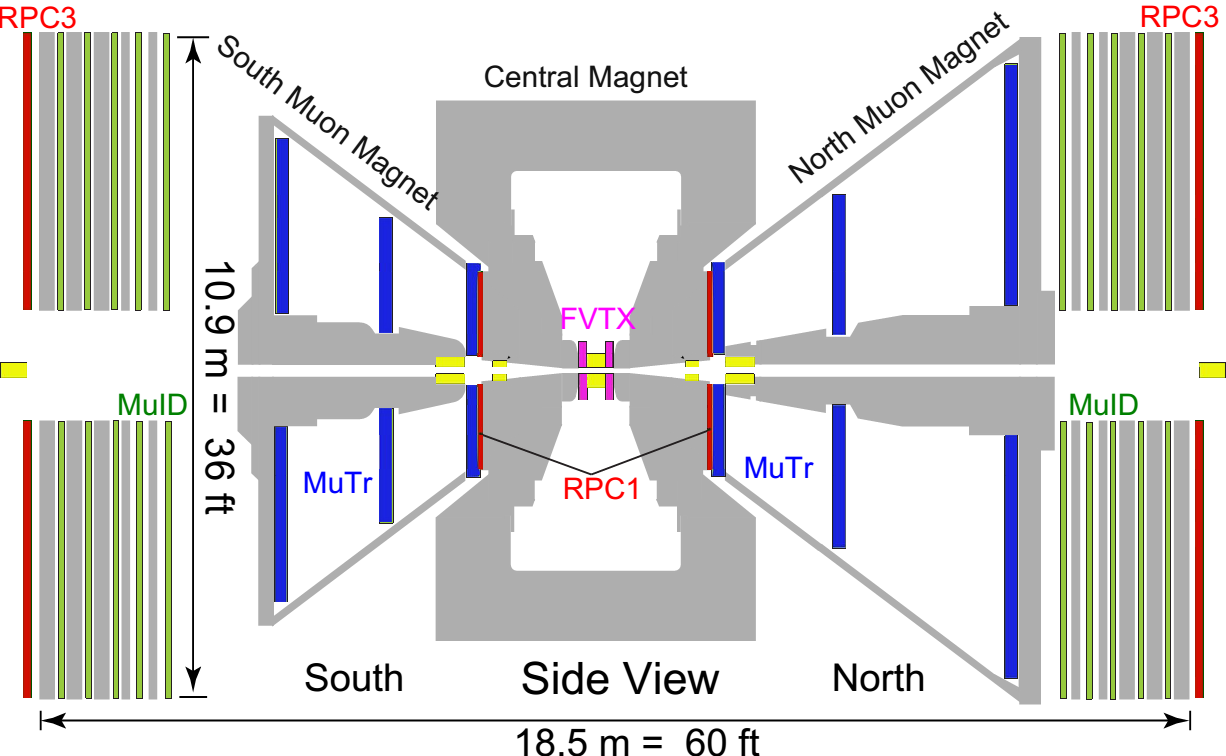
\includegraphics[width=0.8\linewidth]{./figures/phenix_2013_config_muon_arms}
    \caption{Forward Muon Arms}
    \label{fig:phenix_forward}
  \end{subfigure}
  \caption{
    Shown: The two main halves of the PHENIX Spectrometer. The central arms are
    shown via the beam-on view of PHENIX (left) and Forward Muon Arms are shown
    via the 90-degree rotated view. In both cases, the 2013 configuration is
    shown. The beams are brought into intersection at the geometric center of
    each figure (immediately between the BBCs)
  }
  \label{fig:phenix_2013_config}
\end{figure}

PHENIX makes use of many classic detector technologies, it contains \v{C}erenkov
light detectors, resistive plate chambers, electromagnetic calorimeters, silicon
chip detectors, time of flight detectors, scintillation light detectors, cathode
strip chambers, and proportional tube counters.

While all of these subsystems are interesting, and have produced excellent
physics results, I will focus only on those pertinent to this analysis.

PHENIX is generally thought of as two `halves', which often are used in separate
analyses--the forward muon arms, and the central arms. While both halves are
used for both heavy ion, and spin physics analyses, this analysis exclusively
uses the forward muon arms, so the central arms will not be discussed (though, a
closely related analysis, dealing with $A_L$ for $W\rightarrow e$ exclusively
uses the central arms). The different subsystems cover different rapidity
ranges, so many times, complimentary results are obtained from central and
forward analysis. Results from such a complementary central analysis will be
presented alongside my results in later chapters.

PHENIX also utilizes a complex data acquisition system (DAQ) which streams data
from each detector, assembles this data into a labeled event, compresses and
stores into a proprietary storage format, the work-flow of this is summarized in
Figure~\ref{fig:phenix_daq_overview}. A complete summary of PHENIX detector
subsystems (excluding the Forward Vertex Detector, Silicon Vertex Detector, and
Resistive Plate Chambers, which are new, and discussed separately) can by found
in Table~\ref{tab:phenix_detector_summary}.

\begin{figure}
  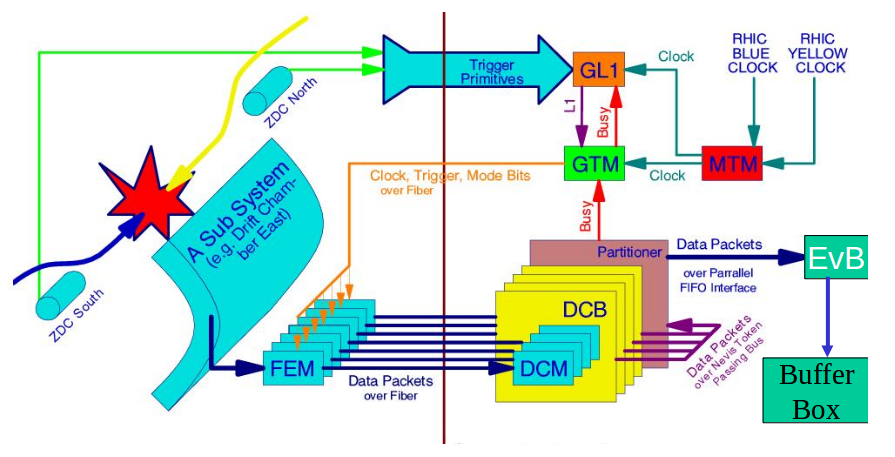
\includegraphics[width=\linewidth]{./figures/daq_overview}
  \caption{ 
    A flow chart summarizing the PHENIX DAQ \cite{Desmond2016}. From left to
    right, we can get a feel for the data flow at PHENIX. Shown is an event, the
    red splat on the far left. Particles from this event are transduced by a
    detector (`A Sub System'). The transduced signals are serialized into a
    detector specific data stream, such that the state of the detector's
    excitation can be recorded and reproduced later. This information is stored
    on the front-end-electronics modules (FEMs), and synchronized with timing
    information from the clock (ticks once every time there is a bunch crossing)
    and a Global Trigger decision, i.e. whether or not the right parts of the
    detector lit up to make this particular event worth keeping. After this, if
    the event is deigned by the heuristics to be worthy of keeping, the
    uncompressed serialized information is sent to the DCMs, where it is
    assembled into a packet, and then sent to the event builder (EvB), where all
    packets sharing a common collision are assembled into an event. The event is
    compressed into a proprietary PRDF format, and sent to the Buffer Boxes,
    which are a cache of high density local storage, which is later sent off to
    cold storage on magnetic tape drives.
  }
  \label{fig:phenix_daq_overview}
\end{figure}

\begin{table}
  \centering
  \begin{tabular}{l c c l}
    \toprule
    \textbf{Element}	& \textbf{$\Delta\eta$}	& \textbf{$\Delta\phi$} & \textbf{Features} \\
    \midrule
    \textbf{Magnets} & & & \\
    Central Magnet & $\pm 0.35$ & $360^{\circ}$ & 1.15 $T$ \\ 
    Muon Magnet North & $-1.1$ - $-2.2$ & $360^{\circ}$ & 0.72 $T$ \\
    Muon Magnet South & $1.1$ - $2.4$ & $360^{\circ}$ & 0.72 $T$ \\
                      & & & \\
    \textbf{Minimum Bias} & & & \\
    Beam Beam Counter & $\pm(3.1-3.9)$ & $360^{\circ}$ & Vertex Reconstruction \\
    Zero Degree Calorimeter & $\pm 2 mrad$ & $360^{\circ}$ & Minimum Bias Trigger \\
                            & & & \\
    \textbf{Central Detectors} & & & \\
    Drift Chambers & $\pm0.35$ & $90^{\circ}\times2$ & Central $p$ and $m$ resolution \\
    Pad Chambers & $\pm0.35$ & $90^{\circ}\times2$ & Pattern Recognition, Tracking \\
    Ring Imaging \v{C}erenkov & $\pm0.35$ & $90^{\circ}\times2$ & Electron ID \\
    Time of Flight & $\pm0.35$ & $45^{\circ}$ & Hadron ID, $\sigma<100pm$ \\
    PbSc EMCal & $\pm0.35$ & $90^{\circ}$, $45^{\circ}$ & Calorimetry, photon, \\
               & & & and electron energy \\
    PbGl EMCal & $\pm0.35$ & $45^{\circ}$ & $e^{\pm}$, $\mu^{\pm}$ separation at $p> 1 GeV/c$ \\
               & & & EM Shower and $p < 0.35 GeV$, $K^{\pm}$ \\
               & & & $\pi^{\pm}$ separation up to $1 GeV/c$  \\
               & & & \\
    \textbf{Muon Arms} & & & \\
    Muon Tracker South & -1.15 to -2.25 & $360^{\circ}$ & North installed 2003 \\
    Muon Tracker North & 1.15 to 2.44   & $360^{\circ}$ &  \\
    Muon ID South & -1.15 to -2.25 & $360^{\circ}$ & Steel absorbers, larocci tubes \\
    Muon ID North & 1.15 to 2.44   & $360^{\circ}$ & "" \\
    \bottomrule 
  \end{tabular}
  \caption{
    A summary of PHENIX hardware~\cite{Adcox2003}. Electron/pion separation and
    Pion/Kaon separation requires the Time of Flight (ToF) working with PbGl and
    PbSc data. PbGl refers to ``Lead Glass Scintillator'' and PbSc refers to ``Lead
    Scintillator''. The Muon Identifier (Muon ID, MuID) can help separate muons
    from hadrons. 
  }
  \label{tab:phenix_detector_summary}
\end{table}

\subsection{The Spin Program}
The PHENIX spin program was planned as part of the RHIC upgrade to produce
polarized proton beams. The major analysis thrust of the PHENIX spin program has
been to understand the spin structure of the proton, and has historically used
various flavors of particle production asymmetries (left-right and
forward-backward) as an experimental probe for polarized parton distribution
functions (as we saw in Chapter~\ref{ch:modeling_proton_spin}).

Much of PHENIX collaboration's early published work focused on creating and
studying quark gluon plasma in heavy ion collisions, but in following years spin
papers came too. Major question in physics that PHENIX set out to answer with
its heavy-ion program include studying confinement--i.e.  why are quark color
charges confined to exist in the nucleus, baryons and mesons? PHENIX sought to
study this via examination of the J/$Psi$ and measuring screening length in
heavy ion collisions. Additional research topics included the study of chiral
symmetry restoration, thermal radiation of hot gasses, QCD Phase transition,
Strangeness and Charm Production, Jet Quenching, and Space-time
evolution~\cite{Nagamiya1994} .

The spin program came shortly after the 2001 commissioning run. The first
polarized proton run was produced by RHIC for PHENIX in 2002, with 8.3 total
weeks of data, run discontinuously. The primary goals of the PHENIX spin
program are to study the polarization of the proton, specifically in the context
of the Ellis-Jaffe sum rule, which decomposes the proton spin into various
contributions from its substructure. The main structures studied by PHENIX are
the gluon polarization, $\Delta g$ and the anti-quark polarization, $\Delta
\bar{q}$. Additionally, the 'nature of parity non-conservation itself can be
directly studied' using polarized beams, and spin asymmetries in collisions.
Though this measurement generally requires a means of reconstructing jets
(PHENIX doesn't have this), inclusive or leading particle production can be used
as a substitute with some small asymmetry
remaining~\cite{PHENIXCollaboration1998}.

\subsection{Subsystems}

The major subsystems contributing to this work include the Muon Arms, the Beam
Beam Counters (BBCs), and the Forward Vertex Detector, since the analysis is
totally characterized with calculating the $A_L$ for $W\rightarrow\mu$
interactions, only muon reconstruction and identification is required. The
Central arms are used in the $W\rightarrow e$ analysis. 

\subsubsection{Beam Beam Counters}

The Beam-Beam counters (BBCs, Figure~\ref{fig:bbc_overview}) are photomultiplier
tubes with scintillating lead-glass crystals. These detectors are situated about
144 cm on either side of the nominal center of the PHENIX interaction region,
and typically are used to trigger on events with minimal bias towards any
particular physics goal. This is important as a means for reconstructing the
relative abundance of particle production, which is as you might expect, crucial
for determination of any inelastic scattering cross section. The Beam-Beam
counters provide us with vertex reconstruction by way of analyzing the time
delay between triggering of the North BBC and the South BBC. The delay window is
then used to reconstruct the event vertex by assuming particles are traveling
at near light speed, Figure~\ref{fig:bbc_vertex_reconstruction}. 

\begin{figure}[ht]
  \centering
  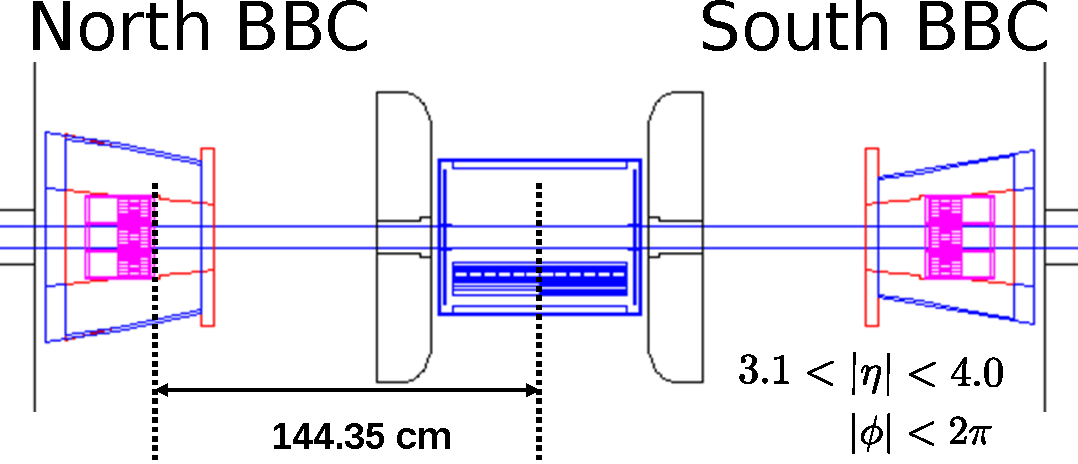
\includegraphics[width=\linewidth]{./figures/bbc_overview}
  \caption{
    Shown: a photograph of the BBC hugging the beryllium beam pipe near the
    center of PHENIX (top left), a schematic showing the relative size and
    location of the BBCs as compared to the rest of PHENIX (top right), and a
    schematic of the exact proportions of the detector as viewed alongside the
    beam pipe (bottom), along with the rapidity and azimuthal
    coverage~\cite{Nakamura2002}
  }
  \label{fig:bbc_overview}
\end{figure}

\begin{figure}[ht]
  \centering
  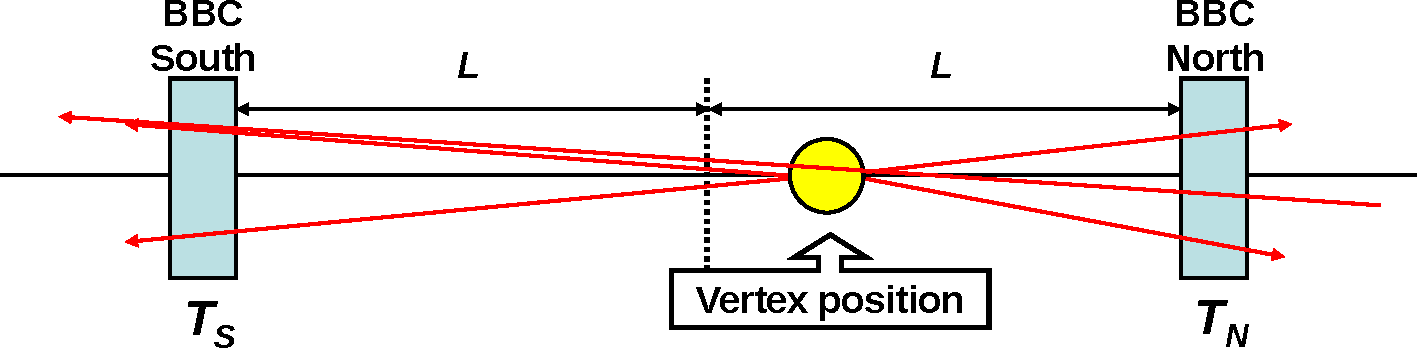
\includegraphics[width=\linewidth]{./figures/bbc_vertex_reconstruction}
  \caption{
    A diagram outlining the strategy for reconstructing the event z-vertex of a
    collision. Top: a cartoon of the North and South BBCs getting some particle
    penetration after an event. Bottom Right: a characteristic distribution of
    measured z-vertices for a short run taken in 2002~\cite{Nakamura2002}.
  }
  \label{fig:bbc_vertex_reconstruction}
\end{figure}


\clearpage
\subsubsection{Forward Vertex Detector}

The Forward Vertex Detector, Figure~\ref{fig:forward_vertex_detector} is a
silicon detector, which provides additional tracking to detect secondary event
vertices and additional precision to the Muon Tracking system. This detector can
provide an important additional layer of precision, because it can help to
identify events which do not originate from the primary event vertex of a
collision, so they can be rejected from a pool of candidate $W\rightarrow\mu$
events~\cite{Aidala2014}. The properties of this detector are summarized in
Table~\ref{tab:fvtx_properties}

\begin{table}[ht]
  \centering
  \begin{tabular}{lc}
    \toprule
    \textbf{Property} & \textbf{Value}\\
    \midrule
    Silicon sensor thickness ($\mu$m) &	320\\
    Strip pitch ($\mu$m) &	75\\
    Nominal operating sensor bias (V)	& +70\\
    Strips per column for small, large wedges	& 640, 1664\\
    Inner radius of silicon (mm) &	44.0\\
    Strip columns per half-disk (2 per wedge) &	48\\
    Mean z-position of four stations (mm)	& ±201.1, ±261.4, ±321.7, ±382.0\\
    Silicon mean z offsets from station center (mm) & 	±5.845, ±9.845\\
    \bottomrule
  \end{tabular}
  \caption{
    A brief summary of the FVTX design parameters~\cite{Aidala2014}
  }
  \label{tab:fvtx_properties}
\end{table}

\begin{figure}[ht]
  \centering
  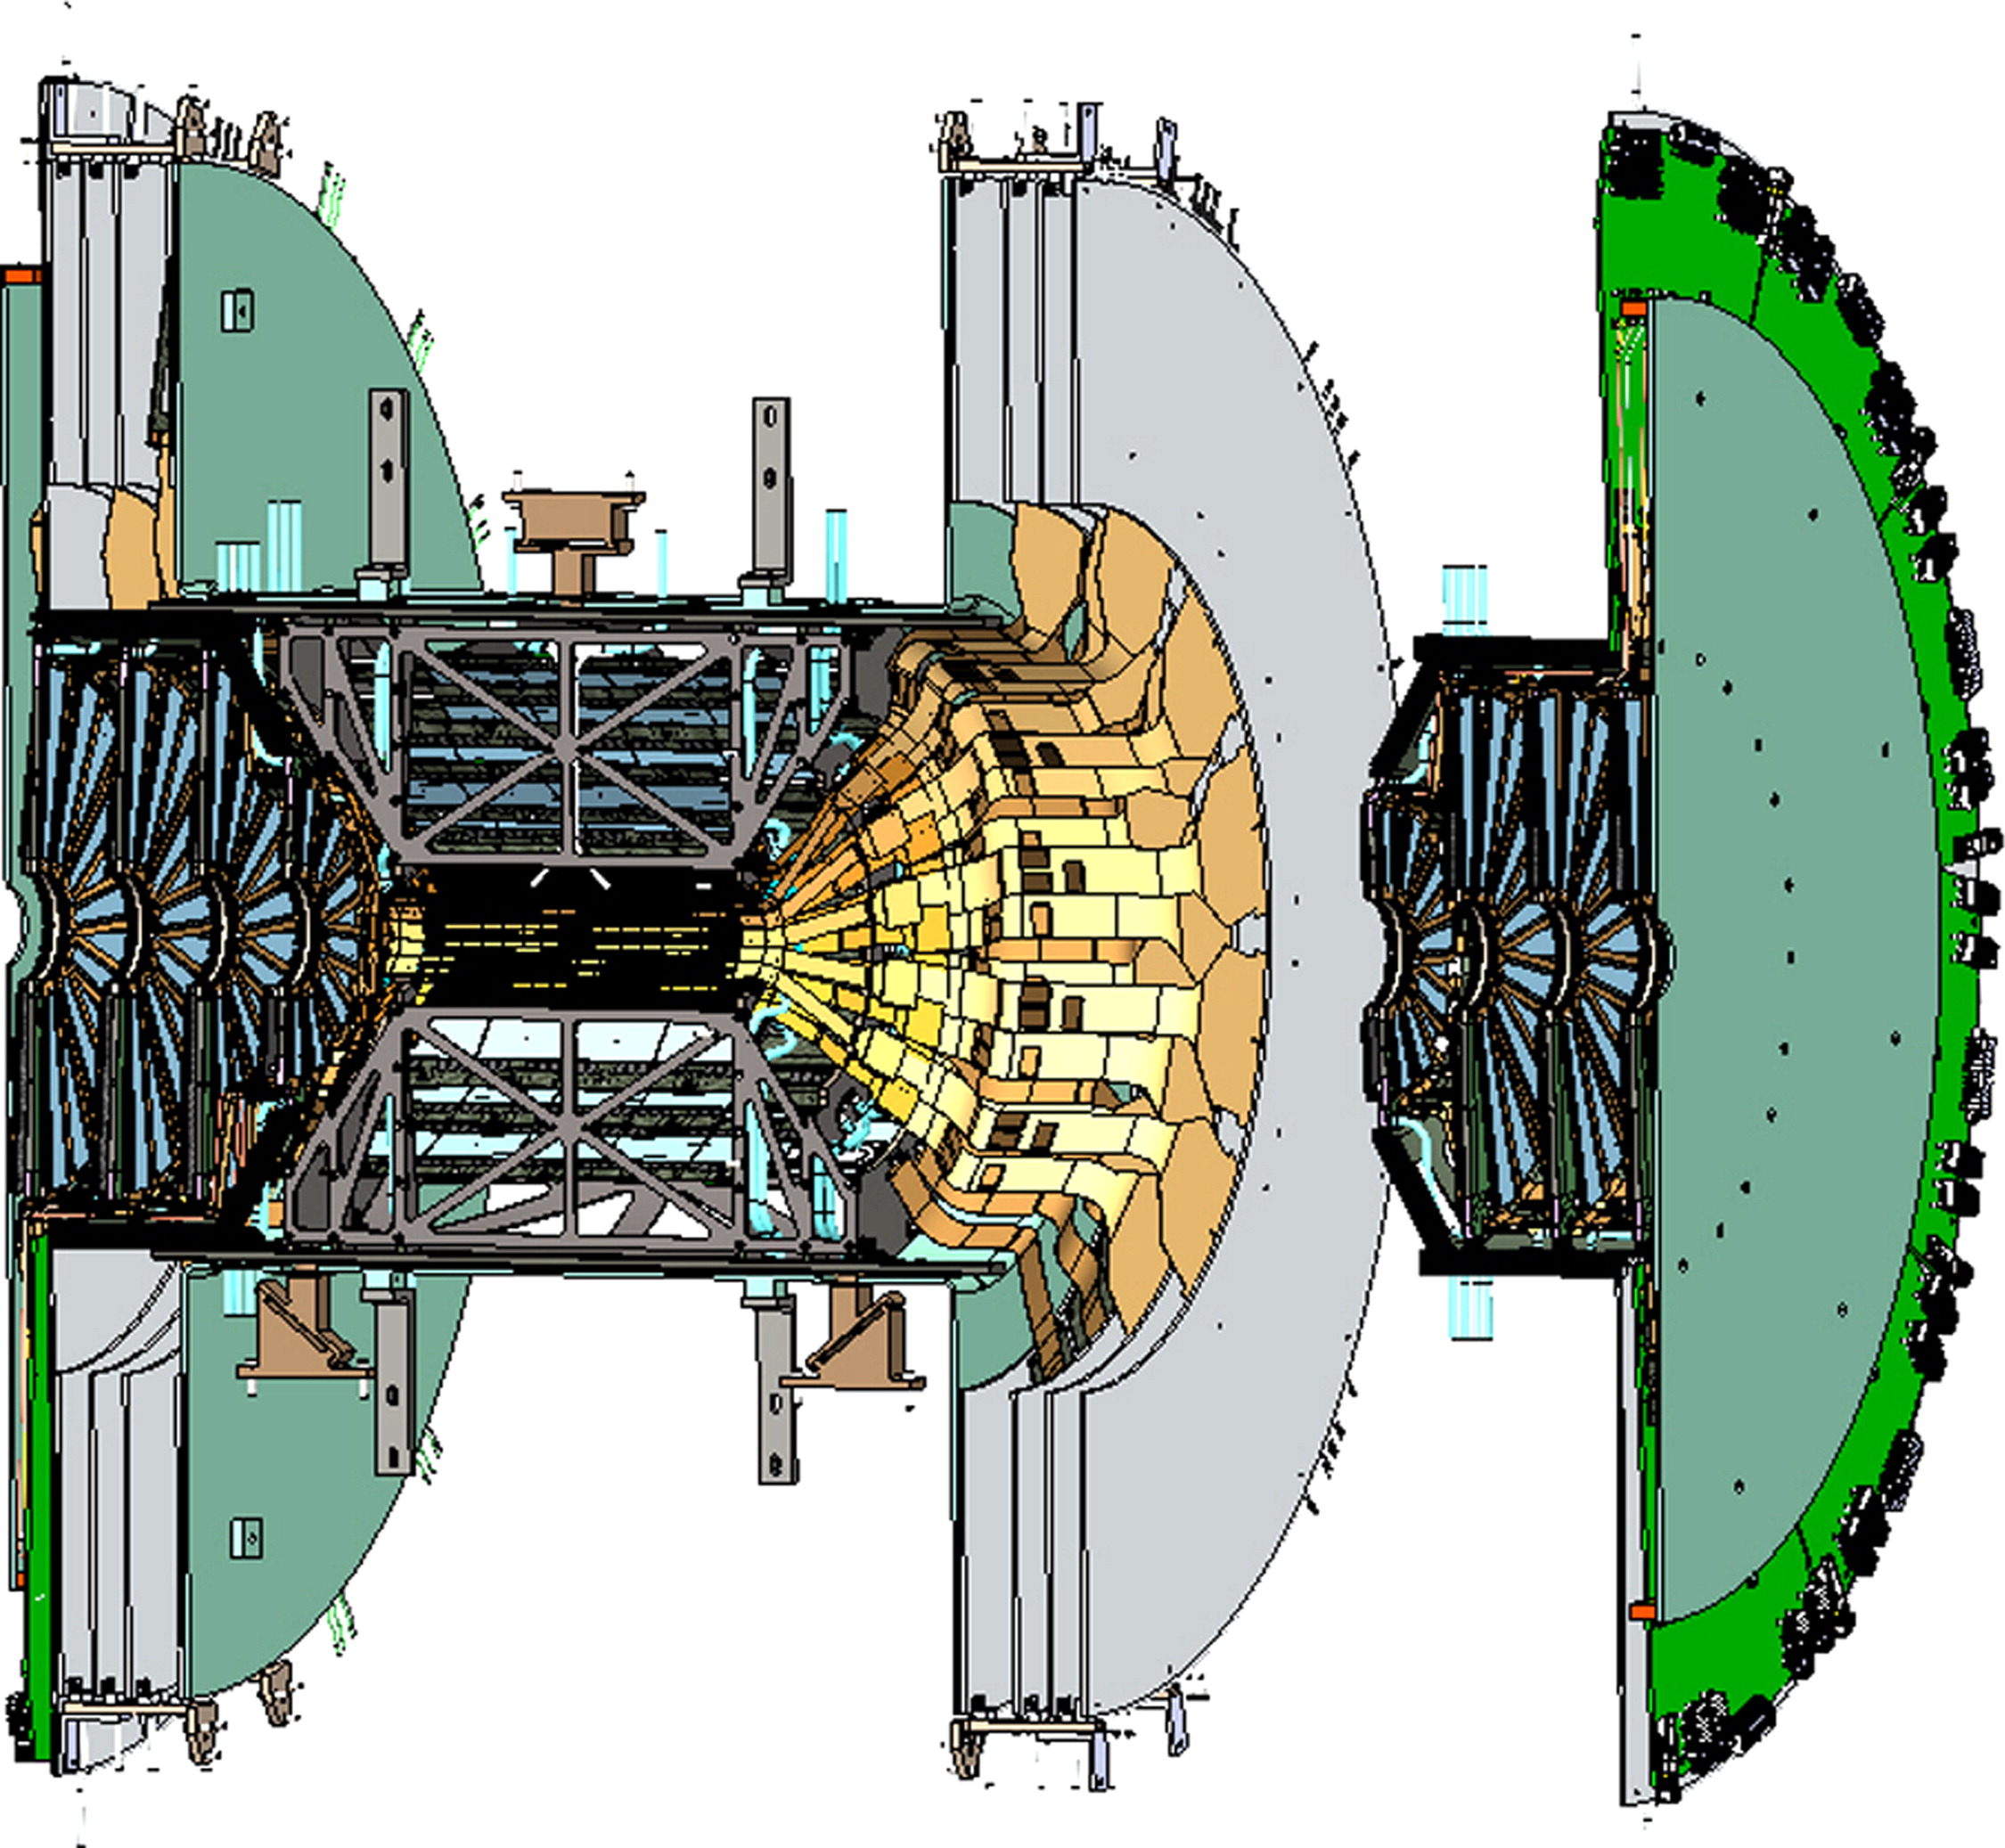
\includegraphics[width=0.6\linewidth]{./figures/forward_vertex_detector}
  \caption{
    A schematic of the Forward Vertex Detector, showing the silicon chip layers
    (light blue wedges), and readout electronics (green). They are mounted
    directly onto the Silicon Vertex Detector, which was not used in this
    analysis. The FVTX and SVD together are used in heavy ion
    analyses~\cite{Aidala2014}.
  }
  \label{fig:forward_vertex_detector}
\end{figure}


\clearpage
\subsubsection{The Muon Arms}

The Muon Arms are composed of several subsystems, including the Muon Tracker
(MuTR, cathode strip chambers), the Muon Identifier (MuID, shielding and
scintillation layers), and the Resistive Plate Chambers (RPC(s), bakelite gas
gaps and azimuthal oriented capacitively coupled copper readout strips). The job
of the muon tracker is to identify muons with the penetration through the many
layers of the MuID, and provide momentum and charge reconstruction for muon
tracks. Tracks are matched to the event vertex with Kalman filter during
reconstruction, and can even be matched with FVTX secondary vertices as a means
of rejecting non W-Boson decays. Prior to the Forward Upgrade
(Section~\ref{sec:forward_upgrade}), the muon arms consisted solely of the Muon
Tracker and the MuID. 

The Muon Tracker has a radial magnetic field, leading to charged particles
traversing the tracker to have a helical bend. This was suitable for lower
energy muon tracks, such as muons coming from the J$\Psi$ decay, which was one
of the primary decays targeted in the original design of the muon tracker.

However, these J/$\Psi$ muons have much lower energy then muons which decay from
areal W-Boson production. To extend the muon tracker's usefulness into tracking
these high energy muons, an upgrade to the triggering system was required to
obtain adequate back-ground rejection for the Forward W analysis. The details of
the muon arms will be discussed in the next section.

\clearpage
\section{The Forward Upgrade} 
\label{sec:forward_upgrade}

The muon arms were the subject of significant upgrades from 2011-2013.
New front end electronics were added to improve triggering, and entire new
detector subsystems (The RPCs) were added. The full details of these subsystems
will be discussed in the forthcoming sections (Section~\ref{sec:forward_upgrade}).

One of the main stated physics goals of PHENIX is to constrain the sea-quark
polarization of the proton spin. While this contribution is
expected to be small, it is not because it is expected to be uniformly zero.
Instead, the expectation is that the matter contribution to the quark sea is
strongly positively polarized, while the antimatter contribution is strongly
negatively polarized~\cite{Aidala2005}. Measuring this polarization via $A_L$
(Equation~\ref{eq:w_production_asymmetry}) is the means by which we will
accomplish this. Prior to the Forward Upgrade, we only had results from the
Central $W\rightarrow\mu$ analysis, but to better constrain our models, we
require lower uncertainty in the forward kinematic regime--thus, the Forward
Upgrade.

The first data for this measurement was taken in 2009, and published in 2010
under \cite{Adare2010} and \cite{Okada2010}, but only for central rapidities,
where a clear Jacobean peak could be found in the electron invariant mass
spectrum at 40$GeV$ mass-energy (half the rest mass of the W-Boson). This made
evaluating yields and calculating asymmetries relatively straight-forward. 

However, in forward kinematic regimes, it was very difficult to discriminate
real $W\rightarrow\mu$ from other sources $X\rightarrow\mu$. As one can observe
in Figure~\ref{fig:muon_production_vs_pt}, only at high $p_T$ does the W-boson
signal become dominant. The old muon trigger electronics did not allow
triggering sufficiently close to the W-Boson production threshold to allow for
enough data to be taken. This is because of how the Muon Tracker identifies the
charge and momentum of particles--which is via track bending. As tracks become
very straight (i.e. high $p_T$), the muon tracker struggles to reconstruct the
correct charge and momentum. The original Forward Upgrade called for a nose-cone
calorimeter, which would have helped greatly for particle rejection, but was
canned for budget reasons.

The Forward Upgrade to PHENIX increased the muon triggering threshold from about
2 $GeV$ to 10 $GeV$, enough to insure that all muons produced from W-Boson
decays can be recorded, with no loss of statistics. This of course is not to
say, that these events were recorded without any background processes--the
removal of the muon background was a substantial effort in this analysis,
described in Section~\ref{sec:sbr}.

\begin{figure}[ht]
  \centering
  \begin{subfigure}[b]{0.5\textwidth}
    \centering
    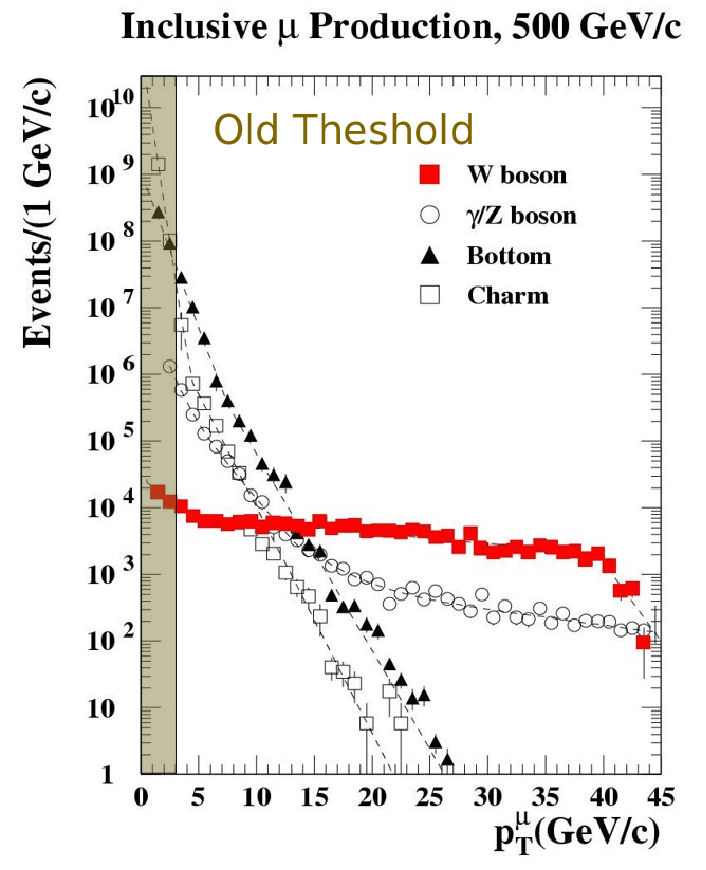
\includegraphics[width=\textwidth]{./figures/w_old_trigger.png}
    \caption{The original Muon Trigger Threshold}
    \label{fig:trig_muon_old}
  \end{subfigure}%
  ~
  \begin{subfigure}[b]{0.5\textwidth}
    \centering
    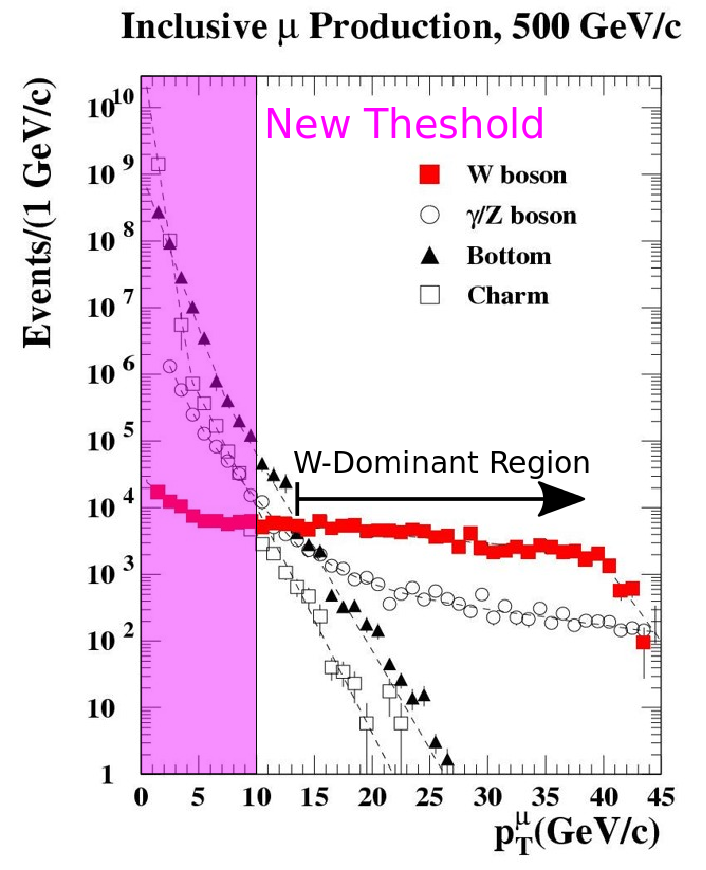
\includegraphics[width=\textwidth]{./figures/w_dominant_region_new_trigger.png}
    \caption{Muon Trigger Threshold, Forward Upgrade}
    \label{fig:trig_muon_new}
  \end{subfigure}
  \caption{ 
    Observing the simulated production of muon as a function of $p_T$, we can
    see that in the kinematic region of $W$ production that the dominant sources
    of muons come from other processes. The new PHENIX muon trigger threshold is
    sensitive at 10 $GeV/c$ and above. The threshold is still high enough that
    with other methods, we can record all events which come from the W boson,
    with triggering, whereas with the old threshold, this was impossible.
  }
  \label{fig:muon_production_vs_pt}
\end{figure}

\subsection{The Muon Tracker}

The primary purpose of the Muon Tracker is to reconstruct the energy and
momentum of muons in the forward kinematic regime. Because the MuID is composed
of larocci tubes sandwiched between solid steel sheets, only particles which
penetrate all the layers of the MuID are identified as muons. The Muon Tracker
has three cathode strip tracking planes in a volume of gas, with an applied
radial magnetic field. Each plane has two faces of tracking strips, for six
total tracking readouts total. The arrangement of cathode strips  makes the Muon
Tracker very sensitive to the azimuthal dimension, but coarsely sensitive to the
radial direction. The Muon Arms have three tracking stations for momentum and
charge identification, sandwiched between two RPCS.

Since the MuID will fire on Muons with a 2.5 $GeV$ momentum threshold, it will
trigger very rapidly at high beam energies and luminosities--too fast to record
all data--event rates were in excess of 10 MHz in 2013, with only 2 kHz of DAQ
bandwidth allocated to the W analysis. Thus, before the Forward Upgrade, the
Muon Arms were insufficient. However, additional absorber was installed at the
nose-cone of the muon tracker to block lower momentum particles. The addition of
the RPCs as well as new Front End Electronics Modules allowed for the real-time
calculation of pseudo-momentum to be fed into the trigger decision in order to
provide high rejection power on tracks. These upgrades allowed us to trigger
exclusively on relatively straight tracks, which is consistent with high
momentum particles~\cite{Fukao2011}.

\clearpage
\subsection{The Resistive Plate Chambers}

One of my major contributions to the PHENIX experiment was in the construction
and testing of the RPCs at station 1, in 2012. An exploded view of the RPC is
shown in Figure~\ref{fig:rpc_exploded}. The RPCs were a crucial part of the
W-Physics muon trigger. One primary feature the presence of RPCs add to the
PHENIX triggering system is timing resolution--2 nanoseconds
(Table~\ref{tab:rpc_design_characteristics}). This is crucial, because before
the inclusion of RPCs, the only timing available was that of the BBCs. However -
because the BBCs are minimally biased--they will fire nearly every time there
is a collision--which at high luminosity is far greater than the assigned
bandwidth to the W Physics trigger. The RPC provides local timing information,
which allows the triggering system to record events which trigger the muon arm
system, and not just the BBCs. This has the effect of significantly reducing
backgrounds--by a factor of $>$ 6000~\cite{Fukao2011},
Figure~\ref{fig:rpc_rejection_power}.

\begin{figure}
  \centering
  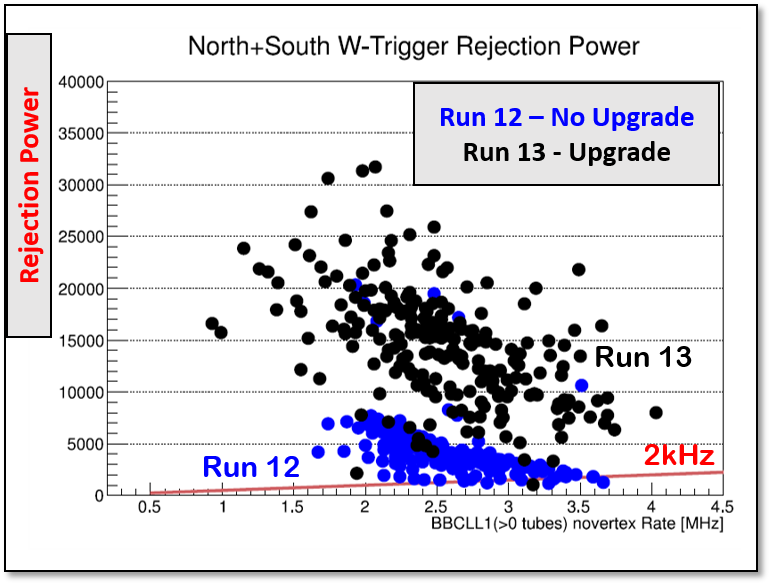
\includegraphics[width=0.8\linewidth]{./figures/rejection_power.png}
  \caption{
    In 2013 with the final commissioning of the RPCs and the Forward Upgrade
    complete, we saw a drastic increase in rejection power, as planned.
  }
  \label{fig:rpc_rejection_power}

\end{figure}


\subsubsection{Design}

\begin{figure}
  \centering
  \begin{subfigure}[b]{0.4\textwidth}
    \centering
    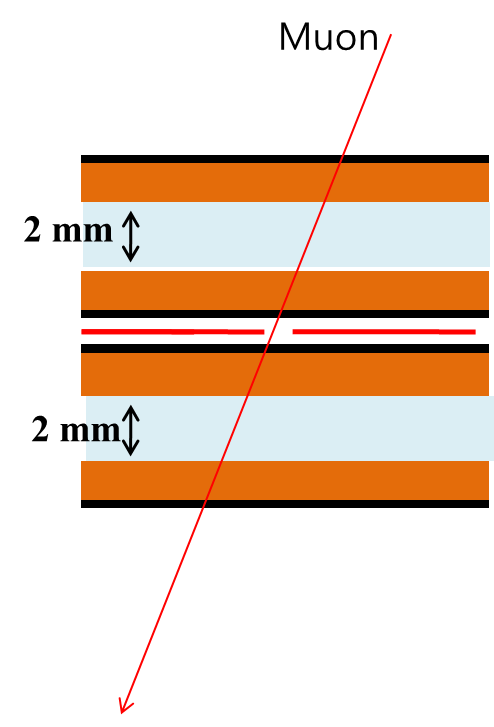
\includegraphics[width=0.8\linewidth]{./figures/rpc_1_muon_hit}
    \caption{A muon passing through the layers of the RPC}
    \label{fig:rpc_hit_side_view}
  \end{subfigure}%
  ~
  \begin{subfigure}[b]{0.4\textwidth}
    \centering
    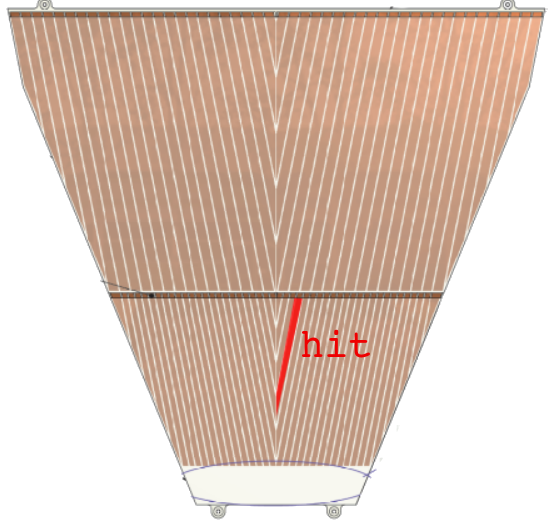
\includegraphics[width=0.8\linewidth]{./figures/rpc_1_muon_hit_side}
    \caption{Copper readout strip activated by passing muon}
    \label{fig:rpc_hit_top_view}
  \end{subfigure}
  \caption{
    As a muon passes through the layers of the RPC (left), the gas in the
    bakelite gap is ionized. This charge migrates and collects near the highly
    resistive graphite coating. An image distribution is induced on the
    overlapping readout strip (right), which is passed along its own channel to
    the front-end electronics.
  }
  \label{fig:muon_hit_rpc}
\end{figure}

As hinted at prior, the design goal of the Resistive Plate Chambers is to
provide accurate timing information at high speed in order to build a Trigger
which can record $W\rightarrow\mu$ events. RPCs were first implemented at the
Large Hadron Collider at CERN, and their design has been adopted for use at
PHENIX both because of its high speed, and low cost. In
Figure~\ref{fig:rpc_exploded} the basic design is shown--the means of signal
transduction is via ionizing of gas inside a highly resistive chamber. The
chamber is held at a large bias--at 8.5 kilovolts, such that any ionization
will collect on the interior of the resistive chamber in a fixed, and relatively
static distribution in time (relative to time scales of triggering system
timing, in millionths of a second). This charge distribution is read out by
capacitively coupled copper readout strips, into fast electronics
(Figure~\ref{fig:muon_hit_rpc}). The design requirements of PHENIX is that when
triggered, 2 or fewer clusters (strips) are activated, the efficiency of the
detector must be at least 95\%, the time resolution must be at least 2
nanoseconds, with a particle transduction rate of 500 Hz per square centimeter.
These properties are summarized in
Table~\ref{tab:rpc_design_characteristics}~\cite{Fukao2011}.

\begin{figure}[ht]
  \centering
  \includegraphics[width=0.7\linewidth]{./figures/rpc_exploded.png}
  \caption{
    We can see the various layers that go into the construction of a typical RPC
    segment installed at PHENIX. A High Voltage bias is applied to the graphite
    coating on either side of bakelite gas-filled gaps. Readout strips are
    positioned between the two bakelite gaps. Finally, the entire double-gap
    structure is surrounded by a copper grounding cage, and wrapped in
    insulating mylar~\cite{Fukao2011}.
  }
  \label{fig:rpc_exploded}
\end{figure}

\begin{table}[ht]
  \centering
  \begin{tabular}{lc}
    \toprule 
    \textbf{Cluster Size} & $<$2 strips \\
    \textbf{Efficiency} & $>$95\% for MIP \\
    \textbf{Time Resolution} & $\sim$2 nanoseconds \\
    \textbf{Rate Capability} & 0.5 kHz/$cm^2$ \\
    \bottomrule
  \end{tabular}
  \caption{
    The design characteristics of the RPCs~\cite{Fukao2011}
  }
  \label{tab:rpc_design_characteristics}
\end{table}

\subsubsection{Construction and Testing}

Construction of the Resistive Plate Chambers took place in two stages over
several years. Fabrication of the bakelite gas gaps was done overseas in Korea,
and the aluminum chassis was manufactured in China. Pieces for the RPC 3 and RPC
1 were shipped to Brookhaven National Laboratory where they were assembled and
tested, before being installed. The installation occurred over two years, with
the first stage, the RPC 3, being installed in 2011, and the second stage, the
RPC 1, being installed in 2012. After being fully commissioned, the capstone
data set for W-Physics was taken in 2013, which is discussed in detail in
Chapter~\ref{ch:data_collection}.

The RPC 3 and RPC 1 construction efforts took place in a special clean-room
built inside of the cavernous building 9-12 (Figure~\ref{fig:building_912}) at
Brookhaven National Lab. Construction was overseen by Dr. Francesca Giordano,
working as a post doctoral associate for Dr. Matthias Grosse Perdekamp for the
University of Illinois at Urbana Champagne. The electronics of the RPCs were
funded by professors Ken Barish and Rich Seto at the University of California,
Riverside, via a grant from the Department of Energy.  I am very grateful for
Francesca for her guidance and trust, as she allowed me to construct and test
many of these octants. I constructed the gaps with Arbin Timilsina, who was a
very entertaining and helpful lab-mate. Ihnjei Choi and Young Jin Kim were
instrumental in the design, construction, and QA of the RPCs as well. 

\begin{figure}
  \centering
  \includegraphics[width=0.5\linewidth]{./figures/building_912_rpc_tent.jpg}
  \caption{
    Two special tents inside building 912 at Brookhaven National Laboratory,
    built to house completed RPC octants and the laboratory used to construct
    and test the octants. 
  }
  \label{fig:building_912}
\end{figure}

The RPCs are modular in design--the larger RPC 3 North and South were separated
into 16 half octants, whereas the smaller RPC 1 North and South were separated
in to eight octants. Both North and South RPCs have the same full azimuthal
coverage, but due to the differing size of the Muon Arms, they have different
rapidity coverage.

The RPC 1 octants were installed directly on the nose-cone of the Muon Tracker,
shown in Figure~\ref{fig:rpc1_installed}. Unlike to the RPC 3, the RPC 1 North
and South are quite compact, and are the exact same size~\ref{fig:mike_in_rpc1}.


\begin{figure}
  \centering
  \begin{subfigure}[b]{0.5\textwidth}
    \centering
    \includegraphics[width=\linewidth]{./figures/rpc1_north_installed}
    \caption{RPC Station 1, North}
    \label{fig:rpc1n}
  \end{subfigure}%
  ~
  \begin{subfigure}[b]{0.5\textwidth}
    \centering
    \includegraphics[width=\linewidth]{./figures/rpc1_south_installed}
    \caption{RPC Station 1, South}
    \label{fig:rpc1s}
  \end{subfigure}
  \caption{
    The North RPC Station 1 is installed on the muon tracker nosecone (left).
    Similarly we see the installation of the south RPC Station 1 (right). The
    metal tube in the center is the beryllium beam pipe.
  }
  \label{fig:rpc1_installed}
\end{figure}

\begin{figure}
  \centering
  \includegraphics[width=0.7\linewidth]{./figures/mike_in_rpc1}
  \caption{
    Here, we see one of the many hard-working physicists who tirelessly worked
    in building 911: a dusty, and irradiated construct built along the AGS
    beam-line. The physicist sits in the center of the RPC1 North chassis, for
    scale. More information can be found in~\cite{Beaumier2016}.
  }
  \label{fig:mike_in_rpc1}
\end{figure}

Each RPC1 octant was hand assembled, with components being tested at each stage
of the construction, where relevant. The first stage of construction involved
preparing the machined aluminum chassis. Mylar sheets were cut to fit the
chassis baseplate, and secured to the aluminum with Kapton tape--chosen for
robustness over high ranges of temperature, as well as good electrical
insulating properties. The chassis itself is not one machined piece, but is
bolted together with machine screws~\ref{fig:rpc1_construction_1}. The chassis
is cleaned several times during the assembly process with methanol to remove any
remaining machining debris.

\begin{figure}
  \centering
  \includegraphics[width=0.7\linewidth]{./figures/rpc1_construction_1}
  \caption{
    The chassis is prepared with insulating Kapton tape and mylar sheeting. The
    grooves along the bottom of the chassis are for routing cabling from the
    readout strips (shown later). The channels along the side of the chassis is
    for routing gas flow lines.
  }
  \label{fig:rpc1_construction_1}
\end{figure}

Double-sided tape is then added to the mylar sheeting, and special foam is then
placed down. Sections are removed from the foam to accommodate routing of the
electrical hookup for setting the Bakelite gas-gaps to a high bias,
Figure~\ref{fig:rpc1_construction_2}.

\begin{figure}
  \centering
  \includegraphics[width=0.7\linewidth]{./figures/rpc1_construction_2}
  \caption{
    Foam shock insulation is added to the RPC 1 chassis.
  }
  \label{fig:rpc1_construction_2}
\end{figure}

After the chassis has been prepared, the bakelite gas gaps are assembled. The
gas gap itself (Figure~\ref{fig:rpc1_construction_3},
Figure~\ref{fig:rpc_exploded}), is composed of two layers of Bakelite, which are
separated by small insulating spacers. On the outside, the Bakelite is coated
with graphite suspended in linseed oil to produce outer surfaces that can be
held at a fixed voltage bias.  The separation of the plates forms a chamber,
which is sealed from the outside.  Electrodes are attached to the linseed oil to
allow for bias, and plastic nipples are routed into the gap chamber allowing for
gas flow. Tubes are cut to size and fixed to the gas chamber nipples, and then
routed out down to the widest end. These gas feed tubes are color coded--a
different color for each Bakelite section in the RPC. These gas gaps are
leak/pop tested in the lab.  This test involved pressurizing the gaps to 8.5
inches of water, and measuring pressure loss over a ten minute interval, using
Argon. Pressure losses less than 1 inch was acceptable. During pressurization, I
checked for an audible pop sound, which indicated one of the gap spacers popping
lose. Popping noises, or bad pressure retention would both result in the gas gap
being discarded.  Finally, before installing the gap, the gap was `burnt in', a
process where the gaps were filled with the `physics gas mixture' and then
slowly voltage cycled to operating voltage over 24 hours.

\begin{figure}
  \centering
  \includegraphics[width=0.7\linewidth]{./figures/rpc1_construction_3}
  \caption{
    The assembled Bakelite gas gap, ready for leak/pop testing, followed by burn
    in.
  }
  \label{fig:rpc1_construction_3}
\end{figure}

After the bakelite gas gaps are tested and have passed, they are installed into
the chassis, Figure~\ref{fig:rpc1_bottom_gap_installation}. The chassis is
prepared for installation with the addition of a layer of copper foil, to create
a Faraday cage around the sensitive bakelite gaps. Tabs are left on the copper
foil, such that they can be folded around the inner gaps, but not around the gas
lines. The bias cables and gas lines are routed through the chassis side
channels.

\begin{figure}
  \centering
  \begin{subfigure}[b]{0.5\textwidth}
    \centering
    \includegraphics[width=\linewidth]{./figures/rpc1_construction_4b.jpg}
    \caption{Routing gas line}
    \label{fig:rpc1_bottom_gas_line_detail}
  \end{subfigure}%
  ~
  \begin{subfigure}[b]{0.5\textwidth}
    \centering
    \includegraphics[width=\linewidth]{./figures/rpc1_construction_4.jpg}
    \caption{Gas gap installed}
    \label{fig:rpc1_bottom_gap_installed}
  \end{subfigure}
  \caption{
    The egress port of the gas gap is carefully shielded with tape to prevent
    friction from causing tears, and routed out of the ports machined into the
    bottom of the chassis (right), with the final position of the first gap
    shown on the left.
  }
  \label{fig:rpc1_bottom_gap_installation}
\end{figure}

Once the bottom gas gap has been installed and secured, the copper readout
strips are added, Figure~\ref{fig:rpc1_construction_5}. The strips are oriented
such that two annuli of readout strips are created (azimuthally) when the RPC 1
is installed onto the nose cone of the muon trackers. The readout strips are
designed this way as to offer some rough radial tracking. The copper readout
strips are laminated with mylar, and each is soldered to its own channel, which
are gathered and soldered onto PCB chips. The readout strips are laminated such
that mounting holes in the laminate attach in the same way to each octant, for
consistency.

\begin{figure}
  \centering
  \includegraphics[width=0.7\linewidth]{./figures/rpc1_construction_5}
  \caption{
    The copper readout strips are mounted to the chassis. Each readout strip is
    soldered to a copper wire, which in turn are gathered into readout chips.
  }
  \label{fig:rpc1_construction_5}
\end{figure}

Following the installation of the readout strips, the final two gas gaps are
installed, with their electronics and gas lines routed through the chassis
similarly to the bottom gap, Figure~\ref{fig:rpc1_top_gap_installation}. 

\begin{figure}
  \centering
  \begin{subfigure}[b]{0.5\textwidth}
    \centering
    \includegraphics[width=\linewidth]{./figures/rpc1_construction_6b.jpg}
    \caption{Routing gas lines}
    \label{fig:rpc1_top_gas_line_detail}
  \end{subfigure}%
  ~
  \begin{subfigure}[b]{0.5\textwidth}
    \centering
    \includegraphics[width=\linewidth]{./figures/rpc1_construction_6}
    \caption{Gas gaps installed}
    \label{fig:rpc1_top_gap_installed}
  \end{subfigure}
  \caption{
    The final Bakelite gas gaps are installed on top of the copper readout
    strips. Gas lines are routed similarly to~\ref{fig:rpc1_bottom_gap_installation}
  }
  \label{fig:rpc1_top_gap_installation}
\end{figure}

Finally, the high voltage cables are grounded to the chassis and soldered to the
relevant wires leading to the graphite electrodes on the outside of the Bakelite
gas gaps. Wires, tubes, etc. are all fixed in place with Kaptan tape. The top of
the chassis is screwed into place, and the front-end electronics are installed,
with the copper readout chips plugging into the relevant FEM board. Ribbon
cables are appropriately routed, and all electronics are encased in copper foil,
and then additionally protected with aluminum shells,
Figure~\ref{fig:rpc1_final_assembly}.

\begin{figure}
  \centering
  \begin{subfigure}[b]{0.5\textwidth}
    \centering
    \includegraphics[width=\linewidth]{./figures/rpc1_construction_7}
    \caption{Inside Assembly Complete}
    \label{fig:rpc1_assembled}
  \end{subfigure}%
  ~
  \begin{subfigure}[b]{0.5\textwidth}
    \centering
    \includegraphics[width=\linewidth]{./figures/rpc1_construction_8}
    \caption{Front-End Electronics Installed}
    \label{fig:rpc1_fem_installed}
  \end{subfigure}
  \caption{
    A completed RPC 1 octant, interior assembly complete, left, and the outer
    assembly completed on the right.
  }
  \label{fig:rpc1_final_assembly}
\end{figure}

After assembly, the RPCs were subjected to a barrage of tests, using a cosmic
ray test stand to measure clustering (Figure~\ref{fig:rpc_cosmics_test_stand}),
designed to measure the activation threshold (combined with energy readings from
scintillators above and below the test stand), determine the average cluster
size, and measure overall detector efficiency. The overall ohmic 'dark-current'
was also measured.

\begin{figure}
  \centering
  \includegraphics[width=\linewidth]{./figures/rpc_cosmics_test_stand}
  \caption{
    Left: the cosmic test stand setup. RPC octants were sandwiched between
    scintillators to run performance and efficiency tests. An example of the
    clustering due to a cosmic ray is shown on the right, with a particle (red)
    activating one or two strips per octant (activation shown in green).
  }
  \label{fig:rpc_cosmics_test_stand}
\end{figure}

\subsubsection{Performance}

With the construction and installation of the RPCs and new Front End Electronics
for the Muon Tracker, PHENIX was ready to take data for the W measurement by
2013. A dedicated run was taken, accumulating over $200 pb^-1$ of data. All
tolerances and design specifications for the upgrade were met.

\subsection{Triggering and Data Acquisition}

The new triggering scheme incorporating the RPCs and the new FEEs is summarized
in Figure~\ref{fig:new_muon_trigger}, while the final configuration of the
PHENIX detector after the forward upgrade is show in
Figure~\ref{fig:muon_arms_upgrades}. As discussed, data was recorded at about
30\% of the total PHENIX DAQ bandwidth of 8 kHz over the 2013 polarized
proton+proton run, which was sufficient to record every single $W\rightarrow\mu$
event. This speaks to the relative rarity of this event, as compared to other
events--the overall collision rate for protons at $510 GeV/c^2$ is as high as
10 MHz.

\begin{figure}[ht]
  \centering
  \includegraphics[width=0.8\linewidth]{./figures/new_muon_trigger.png}
  \caption{
    A schematic of the new muon trigger for recording
    W-Bosons~\cite{Fukao2011}
  }
  \label{fig:new_muon_trigger}
\end{figure}

\begin{figure}[ht]
  \centering
  \includegraphics[width=0.8\linewidth]{./figures/muon_arms_upgrades.png}
  \caption{
    The position of the Front-End Electronics upgrades and new RPCs + Absorber
    are shown. Muon tracker stations are shown in blue (along with the front-end
    electronics). The RPCs sandwich the muon tracking stations and the MuID.
    The absorber material sits just inside of the muon arms, before the Forward
    Vertex Detectors and inner tracking stations of the muon
    tracker~\cite{Fukao2011}
  }
  \label{fig:muon_arms_upgrades}

\end{figure}

\subsubsection{2013 Data Set Triggers}

In general, when two protons inelastically interact, we do not care about the
particles that are produced because they simply tell us about physics which we
already understand. To learn about new physics, or to test models, we must
devise a way to preferentially record this `interesting'  data, since data
recording bandwidth is limited. A decision must be made within the time scale of
one beam crossing (nanoseconds) whether or not to archive the data which is
produced. This process is called `triggering'. The over all trigger rates must
be recorded, so as to reconstruct the relative abundance of events after the
fact. Once a trigger condition has been satisfied, the entire PHENIX
spectrometer will dump its data into the data stream.

The PHENIX DAQ can accommodate 32 different physics triggers. Any transduced
signal by a part of the PHENIX spectrometer can be, provided the front end
electronics are fast enough, be fed into a global triggering decision. Thus,
PHENIX, like other triggered particle physics experiments can be arbitrarily
configured to record a desired subset of data, from the total data set.

Of the 32 triggers available, one is always set to `Noise' (but not recorded)
and another is set to `CLOCK' which is timed to trigger every beam crossing. No
bandwidth is reserved for these triggers. No bandwidth is reserved for these
triggers. There was one global physics trigger configuration used in the Run 13
data set, it was called 'PP510Run13'. An example configuration is shown in
Table~\ref{tab:typical_run}.

\begin{table}
  \centering
  \scalebox{0.8}{
    \begin{tabular}{lrrr}
      \toprule
      \textbf{Name}&\textbf{Scale Down}&\textbf{Raw Trigger Rate}&\textbf{Livetime} \\
      \midrule
      BBCLL1(\textgreater0 tubes) & 31141 & 1921013.65 & 0.89 \\
      BBCLL1(\textgreater0 tubes) novertex & 6732 & 3196505.83 & 0.89 \\
      ZDCLL1wide & 6227 & 370696.78 & 0.9 \\
      BBCLL1(noVtx)\&(ZDCN$\vert\vert$ZDCS) & 6396 & 1498978.93 & 0.9 \\
      BBCLL1(\textgreater0 tubes) narrowvtx & 4070 & 925279.35 & 0.89 \\
      ZDCNS & 4411 & 233334.89 & 0.89 \\
      ERT\_4x4b & 0 & 93.22 & 0.88 \\
      ERTLL1\_4x4a\&BBCLL1(noVtx) & 0 & 490.47 & 0.89 \\
      ERT\_4x4c\&BBCLL1(noVtx) & 1 & 2191.87 & 0.9 \\
      SG3\&MUID\_1H\_N$\vert\vert$S & 95 & 14830.21 & 0.88 \\
      ERTLL1\_E\&BBCLL1(narrow) & 1 & 1039 & 0.9 \\
      CLOCK & 46765 & 9388833.68 & 0.89 \\
      MPC\_B & 0 & 263.11 & 0.89 \\
      MPC\_A & 0 & 1511.4 & 0.89 \\
      MPC\_C\&ERT\_2x2 & 0 & 189.37 & 0.9 \\
      (MPCS\_C\&MPCS\_C)$\vert\vert$(MPCN\_C\&MPCN\_C) & 0 & 10.19 & 0.63 \\
      ((MUIDLL1\_N2D$\vert\vert$S2D)$\vert\vert$(N1D\&S1D))\&BBCLL1(noVtx) & 0 & 260.64 & 0.63 \\
      (MUIDLL1\_N1D$\vert\vert$S1D)\&BBCLL1(noVtx) & 55 & 20196.39 & 0.87 \\
      RPC1+RPC3\_S & 359 & 23841.89 & 0.9 \\
      RPC1+RPC3\_N & 539 & 72270.55 & 0.9 \\
      SG3\&RPC3\&MUID\_1D\_N$\vert\vert$S & 2 & 5526.47 & 0.86 \\
      SG1+RPC1(C)\&MUIDLL1\_N$\vert\vert$S & 0 & 146.32 & 0.86 \\
      MUON\_S\_SG1\_RPC3A\&MUID\_S1D & 0 & 31.27 & 0.89 \\
      MUON\_N\_SG1\_RPC3A\&MUID\_N1D & 0 & 74 & 0.84 \\
      MUON\_S\_SG1\&BBCLL1(noVtx) & 2697 & 323237.99 & 0.9 \\
      MUON\_N\_SG1\&BBCLL1(noVtx) & 11128 & 1095764.77 & 0.9 \\
      MUON\_S\_SG1\_RPC3\_1\_B$\vert\vert$C & 0 & 66.32 & 0.89 \\
      MUON\_N\_SG1\_RPC3\_1\_B$\vert\vert$C & 0 & 173.57 & 0.88 \\
      \bottomrule
    \end{tabular}
  }
  \caption{
    A typical run from the 2013 data set, numbered with PHENIX's standard
    numbering scheme. Each trigger has a descriptive name hinting its
    composition (some triggers are actually constructed from trigger 
    coincidences). Since PHENIX cannot record all data, we see the scale-down,
    the raw rate, and the live-time, which is basically a DAQ triggering
    efficiency.
  }
  \label{tab:typical_run}
\end{table}

The each physics trigger is conveniently stored as a 32-bit integer. This is a
very special integer, because it does not take on all possible values that a
32-bit integer can take on. A trigger with a bit-number of '2' means that the
second binary digit of the trigger's binary representation is flipped to "1" and
the rest of the digits are ``0''. In this way, one can easily store and check
which triggers for a recorded event actually fired. Thus, an important variable
called `trigscaled' in this analysis can be created, to track which triggers
which fired on a certain event by taking the bitwise-OR operation between all
binary representations of triggers which fired for that event.

For example, consider a simplified version of this scheme with four assigned
trigger bits. Lets say we have an event where the following triggers fired:

\begin{itemize}
    \item Trigger 1 Fired: 0001
    \item Trigger 3 Fired: 0100
    \item Trigger 4 Fired: 1000
\end{itemize}

The boolean-OR bitwise comparison is then:

\begin{itemize}
  \item Trigscaled: 1101
\end{itemize}

Note how we lost no information regarding which triggers fired for this event.
We can recover later, in code, the trigger mix for every event by using
bitwise-AND operations, so long as we know which triggers were assigned to which
bit, and we have the trig-scaled number.

This bit-masked final number, ones and zeroes, is one of the crucial variables
in all PHENIX data sets (discussed in the next chapter). It is crucial to know
which triggers fired for which event so that the original collision conditions,
and therefore the physics, can be reconstructed. Since each detector subsystem
may not have the same geometric acceptance, trigger acceptance, signal
traducing hardware, triggering, while necessary for taking data, introduces
severe bias into the data set. Knowledge of which triggers fire for each
recorded event gives us the ability to correct for these kinds of biases to
recover the original conditions of the data sample.

\chapter{Data Wrangling}
The work discussed in this chapter was done in close collaboration with Dr. Ralf
Seidl, Dr. Francesca Giordano, Daniel Jumper, and Abraham Meles. Eventually the
analysis group merged with another year's analysis group, bringing in Dr. Sanghwa
Park, and Dr. Chong Kim, who have made crucial contributions to this analysis,
and have studied the complimentary 2012 data set, producing their own PhD theses
on this analysis. Dr. Hideyuki Oide has also heavily influenced the techniques
and work-flow of this analysis, pioneering many of the techniques used here (at
PHENIX at least) for his analysis of the 2011 data set.

\label{ch:data_collection}
\section{Overview}
Although we have discussed in detail the theoretical motivations for the W
physics program, as well as the machines producing the necessary collisions and
recording data produced from these collisions, we have not yet addressed the
form of the data set itself, and the substantial engineering it takes to extract
the signal of interest out of that data set.

The relative abundance of the $p + p \rightarrow W^\pm \rightarrow \mu^\pm +
\nu$ signal events is rather low, compared to the other interactions which may
take place when two protons collide. We must allow several hundred million
proton proton collisions to occur, before we have a high probability of
observing just one W-Boson event. 

We discussed in the previous chapter how careful triggering is employed in order
to ensure that any time this event does occur, it is recorded. This does not
guarantee that we \textit{only} record these events. Background events are still
recored much more frequently than signal events, even with the improved
triggering. The number of $W\rightarrow\mu$ events produced over the 2013 data
set number in the hundreds, while the total number of recorded events is
approximately 15 billion.

This leads to the substantial problem of fishing out the appropriate physics
events from the 15 billion event haystack. Why, I hear you ask, don't we just
have a detector which can record only the W-Boson events of interest?

Because, as a multipurpose spectrometer, PHENIX must be ready to take
all kinds of data, and satisfy many experimental requirements, in addition to
fitting a lot of functionality into a relatively tight budget, as is common for
federally funded research. Although this measurement would have been made
much simpler with a forward calorimeter, we can't simply build and install a
calorimeter the moment that an analysis would benefit from its presence.

So, instead, we must rely on our ingenuity and deep understanding of the data
set, to tease out the results we want to measure.

\section{Raw Data to Reconstructed Parameters}

Any time a PHENIX trigger condition is satisfied, all of the information
recorded by the PHENIX spectrometer are read out from temporary on-detector
memory, and fed into a data stream that eventually is archived as a 'PHENIX Raw
Data File Format' or PRDFF. 

PRDFF data is hierarchical, first being organized by event-type, and
then organized by packet-type.  There are many event types - 'DATAEVENTS'
typically carry the information relevant to a physics analysis, whereas other
event-types carry very important QA information for determining the status of
the RHIC apparatus, the beam, polarization, and PHENIX performance.

Every packet has a header, which contains general information such as what the
packet contains, and in what order that packet was received. Every packet
recorded can be associated with a unique event-sequence number, which specifies
roughly the order in which the event owning the packet was received by the DAQ.
Within a given run number, an event-number is guaranteed to be unique. The
complexity of the packet is limited by the bandwidth available to move data off
PHENIX onto other storage, and the buffers/reconstruction ability of the front
end electronics modules built onto PHENIX subsystems. PHENIX archives data from
the DAQ at a rate of approximately 700 Megabytes per second - or one compact
disk.

Generally, raw PHENIX data is too complex to use straight-away, because minimal
to no reconstruction of physical properties for a certain event is done, due to
hardware limitations and time limitations - some of this raw data is often
directly used in triggering decisions, which must be made once every 106
nanoseconds or faster (the bunch crossing frequency).

The raw data collected from PHENIX undergoes a process called "Data Production",
where physical parameters are reconstructed from the simpler raw data. Raw data
could take any form - for example - which cathode strips were activated in an
event in the muon tracker, or, the number of photons counted in a
photomultiplier tube. This information is often combined with extensive survey
information about the geometry of a given detector, the known magnetic field in
a detector, to reconstruct quantities such as momentum, or deposited energy.

Once reconstruction has finished in a Data Production, the data are then
repackaged into ROOT files, often times internally structured into custom output
objects which are associated with a various detector. These output objects are
simply custom written C++ classes which have a serialization scheme, which have
libraries and dictionaries compiled that allow for them to be serialized into
ROOT's file format.

For the purposes of this analysis, all data has been reconstructed and
serialized into a specific type of output object called a 'picoDST' or even more
concisely, 'pDST'. This name, like many others in PHENIX has historical context:
DST stands for 'Data Summary Tape' hearkening back to the days when data was
stored primarily on magnetic tape (it is still archived on magnetic tape!), and
'pico' because of its relatively small disk-space requirement, compared to
'nanoDST' files or simply 'DST' files. I'm not making this up, I swear!

\section{Choosing Analysis Variables}

Even data reduced to the point of a pDST still is much more complicated and
comprehensive than what is needed for this analysis - there are thousands of
variables relating to reconstruction parameters. We only need a handful of
variables for this analysis, summarized on Tables
\ref{tab:evt_variables},\ref{tab:mutr_variables}, \ref{tab:fvtx_variables} and
\ref{tab:rpc_variables}. When Cartesian coordinates are referenced, implicitly,
the reference frame is the PHENIX Coordinate system
(Figure~\ref{fig:phenix_coordinate_system}).

As you can probably guess, the only variables which are truly relevant to this
analysis need to be relevant to understanding two questions:

\begin{enumerate}
  \item \textit{Is this reconstructed muon track the result of a real W-Boson Decay?}
  \item \textit{What is the polarization of the two colliding protons for every recorded collision?}
\end{enumerate}

To properly answer these questions, we need to comprehensively understand what
processes are capable of producing muons, as well as whether or not our detector
can be 'tricked' by signals which look like muons, but really aren't. Secondly,
we need a means of recovering the proton spin polarization for each colliding
bunch-pair.

Polarization recovery is straight-forward - we already have mechanisms in the
data stream which number and track the colliding bunch pairs. We additionally
have well defined spin patterns which are applied to the 120 bunches, the same
way every time this pattern is applied to the fill. As discussed previously, we
have good QA apparatuses in place to ensure the advertised spin pattern is the
same as the delivered spin pattern. Since polarization patterns do not typically
change in a standard physics beam fill (if they do, alarms are raised and the
data is typically discarded), all that is needed is to associate a PHENIX run
number, with a RHIC fill number, and then look up the spin pattern, which in
effect, is a database-call. Of course, the overall beam polarization percentage
is an important factor, which dilutes any spin asymmetry, but this is taken into
account in the final spin database QA analysis~\cite{Kim2014}.

This leaves us with the first question, and the difficulty in answering this
question is essentially that it is challenging to differentiate signal
$W\rightarrow\mu$ events from other $X\rightarrow\mu$ events, or even events
which look like muons, but are really due to incorrect track reconstruction.

Therefore, the thrust of the Data Analysis portion of this work is really just
to tease apart the real W-genic muons, from all other muon candidates. To this
requires some substantial feature engineering, and creating some statistical
models, as well as a means of evaluating the performance of these statistical
models - which is difficult because validating any statistical differentiation
technique (aka machine learning technique) requires a labeled data set, and we
intrinsically do not possess this, since otherwise, this analysis would not need
to be done.

\begin{table}
  \centering
  \begin{tabular}{l p{0.7\linewidth}}
    \toprule
      \textbf{Name} & \textbf{Description} \\
    \midrule
      Run\_Number & A unique number identifying a run in a RHIC fill for PHENIX \\
      Evt\_Number & A unique number within a single run identifying the approximate order an event was taken. \\
      Evt\_bbcZ & The event z-vertex calculated by the BBC \\
      triggerbit & The result of a bit-wise 'OR' applied to all 32-bit trigger bits which fired \\
    clockcross & The bunch number of the two colliding bunches $[0-119]$. Required to look up the spin polarization, along with Run\_Number \\
    \bottomrule
  \end{tabular}
  \caption{Variables characterizing events overall}
  \label{tab:evt_variables}
\end{table}

\begin{table}
  \centering
  \begin{tabular}{l p{0.7\linewidth}}
    \toprule
    \textbf{Name} & \textbf{(Unit) Description} \\
    \midrule
    Evt\_Nmu & The number of muon tracks reconstructed for a given event \\
    charge & ($\pm e$) The charge associated with a reconstructed muon track \\ 
    $p_z$ & (GeV) The z-momentum associated with the muon track \\
    $p$ & (GeV) The total momentum of a charged track \\
    $\chi^2$ & The result of the Kalman fitter reconstructing the track \\
    lastGap & The last gap in the Muon Tracker which was activated (there are 4) \\
    $\eta$ & The rapidity of the track \\
    $\phi$ & (rad) The azimuthal position angle the track makes relative to the x-axis \\
    DG0 & (cm) A Track matching variable (matching between MuID and MuTR) associated with the MuID road, at MuID station 3. \\
    DDG0 & (degree)  The opening angle between the MuID track road, and the MuTr projection onto the MuID \\
    xSta${}_i$ & (cm) The x-coordinate of the track at Station i,  $i\in{1,2,3}$ of the MuTr \\
    ySta${}_i$ & (cm) The y-coordinate of the track at Station i, $i\in{1,2,3}$ of the MuTr \\

    $\phi_i$ & (rad) The angle the track makes with Station i, $i\in{1,2,3}$, i.e.: $\phi_i = tan^{-1}\left({{x_1}\over{y_i}}\right)$ \\
    $\theta$ & (rad) Azimuthal angle of track, $tan^{-1}\left({p_T \over p_z}\right)$ \\
    DCA${}_z$ & (cm) Distance of closest approach between the z-vertex positions extracted by projecting the MuTR track z-vertex back to the BBC z-vertex \\
    DCA${}_r$ & (cm) Distance of closest approach between the track and beam axis \\ 
    \bottomrule
  \end{tabular}
  \caption{
    Muon tracker variables. Generally, this data set is indexed on a subevent 
    level, where one event will contain all reconstructed muon tracks seen for 
    that event.
  }
  \label{tab:mutr_variables}
\end{table}

\begin{figure}
  \centering
  \includegraphics[width=0.7\linewidth]{./figures/dg0_ddg0.png}
  \caption{
    A schematic representation of the matching variables, DG0 and DDG0 at
    the intersection between the Muon Tracker and Muon 
    Identifier~\cite{Oide2012}
  }
  \label{fig:dg0_ddg0}
\end{figure}

\begin{table}
  \centering
  \begin{tabular}{l p{0.7\linewidth}}
    \toprule
    \textbf{Name} & \textbf{Description} \\
    \midrule
    $fvtx_{d\phi}$ & The $\phi$ residual between MuTR track and FVTX track \\
    $fvtx_{d\theta}$ & The $\theta$ residual between the MuTR track and FVTX track \\
    $fvtx_{dr}$ & The radial residual between the MuTR track and the FVTX track \\
    $fvtx_{conebits}$ & The number of FVTX clusters inside a cone around the track defined by: $0.04 rad < dR < 0.52 rad$ where $dR = \sqrt{{d\eta}^2+{d\phi}^2}$\\
    \bottomrule
  \end{tabular}
  \caption{A summary of the variables reconstructed from FVTX raw data~\cite{Meles2015}.}
  \label{tab:fvtx_variables}
\end{table}

\begin{table}
  \centering
  \begin{tabular}{l p{0.7\linewidth}}
    \toprule
    \textbf{Name} & \textbf{Description} \\
    \midrule
    RpcMatchSt1 & Distance of closest approach between projected MuTR track onto the RPC 1 and the closest hit cluster on RPC 1\\
    RpcMatchSt3 & Distance of closest approach between projected MuTR track onto the RPC 3 and the closest hit cluster on RPC 3\\
    \bottomrule
  \end{tabular}
  \caption{RPC Track matching variables}
  \label{tab:rpc_variables}
\end{table}

\begin{figure}
  \centering
  \includegraphics[width=\linewidth]{./figures/phenix_coordinate_system.png}
  \caption{
    The PHENIX coordinate system is shown (RGB arrows) at the center of the
    nominal interaction point within PHENIX, the origin, in this quarter-cutaway
    drawing. The small black figures are actually miniaturized human beings, the
    PHENIX detector is very small - this is a full scale drawing of PHENIX.
    Shown: the x, y, and z coordinates, as well as the azimuthal coordinate,
    $\theta$ and polar coordinate $\phi$ ~\cite{WebPHENIXDrawings}
  }
  \label{fig:phenix_coordinate_system}

\end{figure}


\begin{figure}
  \centering
  \includegraphics[width=0.8\linewidth]{./figures/kinematic_variables_schematic.png}
  \caption{
    A nice summary of discriminating kinematic variables reproduced with
    permission from Dr. Chong Kim. We see the MuTR tracking planes in green, and
    a muon track penetrating the planes in red, and reference coordinates in the
    lower right-hand corner. The geometric relationship between the roads,
    reconstructed track are shown in the annotations.
  }

\end{figure}

The engineered variables in this analysis are $dw_{13}$, $dw_{23}$,
$d\phi_{13}$, and $d\phi{23}$.  These variables are calculated from
reconstructed physics data. They play an important role in our extraction of the
signal to background ratio.  The $d\phi_{ij}$ variables represent the difference
in azimuthal angle observed at the MuTR station i and j respectively.  $dw_{ij}$
is constructed from $d\phi_{ij}$ as follows:
\begin{equation}
  dw_{ij} = p_T \times sin(\theta) \times d\phi_{ij}
  \label{eq:dw23_definition}
\end{equation}

While $\phi_{i}$ is calculated from the x and y coordinates at Station i:

\begin{equation}
  \phi_i = tan^{-1}\left({ySta_i \over xSta_i}\right)
  \label{eq:phi_definition}
\end{equation}

A common theme amongst these variables is that they should help us distinguish
between high momentum muon tracks from W-Bosons, and other muon tracks. The hope
is that the muon tracks from W-Bosons are kinematically restricted to have a
relatively narrow momentum distribution in the forward kinematic regime, and so
therefore, tracking variables can be used to partially differentiate between
signal and background events.

In general, W-genic events will be mostly straight, geometrically, and so this
constrains the values of variables such as DCA${}_r$ substantially, and other
variables less so. Thus, $dw_{23}$ should be a good discriminator, as it depends
on $p_T$ and the azimuthal bending of the charged tracks, due to the radial
magnetic field in the MuTR.

Our secondary requirement of our variables is that they are relatively
uncorrelated with each-other, to leave plenty of room for statistical modeling.
Ultimately, we chose a subset of the available tracking variables to carry out
the analysis, in two stages. The correlation of variables for both data and
simulation are summarized in Table~\ref{tab:kinematic_var_correlations}.

In the first stage of the analysis, we use: DG0, DDG0, DCA${}_r$, $chi^2$,
Rpc1DCA, Rpc3DCA, $fvtx_{dr \times d\theta}$, $fvtx_{d\phi}$, and $fvtx_{cone}$.
Of these variables, some were grouped to account for correlations: DG0 and DDG0,
$\chi^2$ and DCA${}_r$. These variables are all related to track reconstruction.
The Muon Tracker reconstructs tracks by essentially connecting the dots between
x and y coordinate 'hits' that it records at each station. The lines connecting
these hits are called 'roads'. Following this, the roads and hits are used to
generate a curve fit to the data, given knowledge of the muon tracker's radial
magnetic field. From this curve, we extrapolate the charge and momentum, and we
construct variables which codify the difference between the reconstructed curve,
and the 'connect the dots' roads. The smaller these differences are, the more
straight the track is, and as discussed, straightness points to higher momentum,
which ultimately leads to labeling as a W-genic particle, if the momentum is in
the correct range.

In the second phase of the analysis, we use $dw_{23}$ and $\eta$ primarily. Both
stages of the analysis are discussed in the following sections. $dw_{23}$ is
related to track straightness as well, and is referred to as "reduced azimuthal
bending". Since we're interested in forward muons, $\eta$ is used as our second
variable.

Generally, we are interested in recovering forward $\mu+$, forward $\mu-$,
backward $\mu+$ and backward $\mu-$. As the muon arms do not have the same
rapidity coverage, we separate the data into these four categories - forward
positive charged tracks, forward negatively charged tracks, backwards positively
charged tracks and backward negatively charged tracks. Due to the geometry of
the muon arms, the North Arm will always correspond with forward positive
rapdity, whereas the South Arm will always correspond with backward, negative
rapidity. I will use 'forward and backward' interchangably with 'North and
Sout'. We perform all calculations with our data set in parallel between these
four conditions.

The data is further subdivided based on the available track matching variables
for a given event, but these subdivisions are not kept separate from the
overall arm-charge separation. Some variables, such as the RPC track matching
variables and the FVTX track matching variables exist for some events, but not
others. We will discuss how this is managed in later sections, but this data is
not generally partitioned in this way.

\clearpage

\chapter{Feature Engineering}
\label{ch:feature_engineering}
The ultimate goal of Feature Engineering is to clean the data and transform the
data with heuristic strategies that tag events coming from signal sources, as
separate from events which come from our background, so that we can proceed with
the calculation of the physics asymmetry.

Even with the Forward Upgrade (Section~\ref{sec:foward_upgrade}), our data set
is still composed mostly of background events
(Figure~\ref{fig:data_composition}). The primary constituents of the data set
are muons from the following sources:

\begin{itemize}
  \item \textbf{Hadronic Background}
    \begin{itemize}
      \item The hadronic background is composed of hadrons which are produced
        from the primary event vertex, and then travel into the muon arms. The
        hadrons then decay in the muon arms, and create hits at each station,
        which are mis-reconstructed as high-$p_T$ muons.
    \end{itemize}
  \item \textbf{Muon Background}
    \begin{itemize}
        \item The muon background is composed of processes which produce real
          muons which fall into a similar kinematic regime of the W-genic muons
    \end{itemize}
  \item \textbf{W Signal}
    \begin{itemize}
        \item These are muons we are looking for. They come from the W boson
          decay, and carry information about the proton spin.
    \end{itemize}
\end{itemize}

We will differentiate these types of data in two different step. In the first
step, we will use likelihood event selection, where we lump hadronic background
and muon background together, and merely distinguish it from W-genic events. In
the second stage, we will further differentiate our model for the background,
drawing heavily on the data to understand the hadronic background, and providing
simulations of the W-genic events as well as simulation cocktail for other muon
background events. Before we discuss this differentiation, it is important to
discuss the simulations, as the rest of the analysis hinges on the simulation of
both the W-genic events and the Muon Background events.

\begin{figure}[ht]
  \centering
  \includegraphics[width=0.8\linewidth]{./figures/data_composition.png}
  \caption{
    A cartoon of the dataset composition. The data, even after the Forward
    Upgrade, is mostly composed of hadronic background, which has tricked our
    Muon Tracker.
  }
  \label{fig:data_composition}
\end{figure}

In subsequent sections, I will discuss what we do with the variables which we
have chosen to use to identify W-genic events. Because our data set is so
dominated by background sources, we must rely heavily on simulations to estimate
what our signal events might look like. As of the time of this writing, the
analysis has not yet incorporated the simulation of hadronic background, which
is quite difficult, as there are a lot of effects at play - particles which
interact with the material of PHENIX itself to produce secondary and tertiary
vertices, for example. However, if we can simulate accurately the signal process
(the W-Boson cross section and its scaling with energy is known to excruciating
precision), and the muon background processes (known to similarly high
precision), we can approach the problem from a standpoint of using our data set
as a relatively good model for what 'hadronic background' looks like, and use
simulations to fit the portions of the data which cannot come from this hadronic
background. 

\clearpage
\section{The Basic Cut}

The basic cut aims to remove all obviously bad events from our event mix. The
cut approaches this from two premises. The first, is that if track
reconstruction variables simply cannot have resulted from a W-genic event, then
we remove the track. Secondly, if the track corresponds to a reconstructed
energy which is larger than what is physically allowable for a W-genic track, we
remove it.

The "Basic Cut" is defined:
\begin{table}[ht]
  \centering
  \begin{tabular}{l c c}
    \toprule
    \textbf{Variable} & \textbf{Lower Bound} & \textbf{Upper Bound} \\
    \midrule
    MuID lastGap & * & Gap 4 \\ 
    $\chi^2$ & 0 & 20 \\
    $DG0$ & 0 & 20 \\
    $DDG0$ & 0 & 9 \\
    $\mu$ candidate & * & 1 \\
    \bottomrule
  \end{tabular}
  \caption{ The Basic Cuts used in the Run 13 analysis. lastGap refers to the
    last gap in the MUID which saw a $\mu$ candidate event. The fourth gap is
    the furthest penetration possible, therefore suggesting a high energy muon.
    Other parameters are described in Tables \ref{tab:evt_variables}, 
    \ref{tab:mutr_variables}, \ref{tab:fvtx_variables}, and
    \ref{tab:rpc_variables}
  }
  \label{tab:basic_cut}
\end{table}

With this cut, we have removed quite a large fraction of the data, without worry
of removing signal events.

\clearpage
\section{Simulations}

I did not do any work to produce the simulations used in this analysis, all of
that credit goes to Dr. Ralf Seidl. I will generally describe how the
simulations were produced, and paraphrase from the analysis note which we
co-wrote with contributions also from Dr. Giordano, Abraham Meles and Daniel
Jumper:~\cite{Seidl2014}.

PHENIX has a rather well developed simulation framework, which uses the in-house
built "PHENIX Integrated Simulation Application" (PISA)~\cite{Macguire1997}
custom simulation framework. The simulation framework models in great detail the
entire 12mx18mx18m volume of the PHENIX apparatus, as well as all the various
material properties of the apparatus. The software package originated from the
GEANT geometry and tracking packages. PISA encompasses more than this, though,
it additionally encapsulates event-generators, a standalone geometry
verification package, and the PHENIX offline analysis shell, to generate data
that is completely compatible with PHENIX's data packaging framework. PISA has
since been integrated into a simulation work-flow with the popular PYTHIA event
generation system.

The simulations were created by selecting the biggest sources of muon
background known to be produced at PHENIX as well as the W-Boson event and
producing many events to generate good statistics. The primary purpose of
simulating the muon background and W-Signal is to ultimately generate
probability distribution functions for the variables which have the largest
analyzing power - i.e. ability to differentiate between signal and background.
The simulation and data both are ultimately described by the same variables.

The data are added together, when combined to generate a 'muon background pdf'
or 'W-Signal pdf' according to the cross-section of the process and the number
of generated events, so as to not add these ingredients into the cocktail in the
wrong amounts. This process is described in the next section, but the
simulations used in this analysis are summarized here, in
Table~\ref{tab:simulation_cross_sections}. When adding the simulations together,
one must be careful to scale the final-yields by a correction factor (called
k-factor) such that events which produce boosted dimuons are properly accounted
for.

PHENIX uses some somewhat exclusive jargon when describing the various quark
bound states which contribute to the muon background, and signal events.  Open
charm or charmonium refer to the bound state of the $c\bar{c}$ quarks.  Onium
generally refers to any process where a particle is in a bound-state with its
own antiparticle (without of course double-counting open charm/charmonoim).
Direct photon, or alternatively $d\gamma$ (sometimes also written as DY) refers
to photons that are produced as an immediate result of a inelastic scattering
process, not from secondary decays. Open bottom refers to the bound state of
$b\bar{b}$ quarks. Z/$d\gamma$ refers to the production and decay of the mixing
between the Z-boson and virtual photons. ONLY Z refers to Z production and
decay.  W is naturally the signal event. W tau refers to the production of tau
leptons, which can decay weakly, producing electrons or muons. W had refers to
the production of W bosons from hadronic processes, rather than as the primary
event vertex.  All of these processes are summarized in
Table~\ref{tab:simulation_cross_sections}.  
\begin{table}[ht]
  \centering
  \begin{tabular}{ccccc}
    \toprule
    \multicolumn{5}{c}{\textbf{Reference Run 393888}}\\ 
     & & & & \\
    \textbf{Process} & 
    \textbf{k factor} & 
    \textbf{$\sigma$ } & 
    \textbf{\# Events} & 
    \textbf{ $\mathcal{L}$ } \\
    & & (\textit{mb}) &  & ($fb^{-1}$) \\
    \midrule
    $c\bar{c}$ & 2.44  & 5.71e-01 & 5.85e+11 & 1.02 \\
    onium      & 0.415 & 1.35e-01 &  1.5e+11 & 1.11 \\
    $d\gamma$  & 0.0   & 5.32e-02 & 5.84e+10 & 1.10 \\
    $b\bar{b}$ & 1.83  & 7.30e-03 & 7.36e+09 & 1.01 \\
    ONLY Z     & 1.25  & 3.37e-07 & 1.73e+08 & 577.0\\
    W          & 1.5   & 1.66e-06 & 3.38e+08 & 198.9\\
    W tau      & 0.0   & 1.66e-06 & 3.43e+08 & 201.8\\
    W had      & 0.0   & 1.66e-06 & 3.42e+08 & 201.2\\
    Z          & 1.25  & 1.02e-06 & 2.93e+08 & 61.2 \\
    \bottomrule
  \end{tabular}
  \caption{
    Simulated sub processes in Run 13 including their generated event numbers
    as well as the corresponding luminosity and cross sections. Dr. Sanghwa Park
    has done an extensive analysis of the simulated data to determine an
    appropriate k-factor. Process which contribute very little to the muon
    background include W had, W tau, and $d\gamma$; they are scaled to zero.
  }
  \label{tab:simulation_cross_sections}
\end{table}                  


The simulations must additionally be weighted for trigger efficiency. To
accomplish this, we weight events for each arm and charge with the associated
trigger efficiency when constructing probability density functions representing
the muon background. The trigger efficiencies generally manifest as $\eta$
dependent functions - thus we bin the data into 20 separate $\eta$ bins and
calculate the efficiency associated with each bin. The bin ranges, and
efficiency corrections are summarized in
Table~\ref{tab:rapidity_corrections_north} for the North arm, and
Table~\ref{tab:rapidity_corrections_south} for the South arm.
\begin{table}
  \centering
  \begin{tabular}{cccc}
    \toprule
    \multicolumn{4}{c}{\textbf{South Arm}} \\
    \textbf{$\eta_{min}$} & 
    \textbf{$\eta_{min}$} & 
    \textbf{$\mu^{-}\pm stat \pm sys$} & 
    \textbf{$\mu^{+}\pm stat \pm sys$} \\
    \midrule
    1.10 & 1.17 & $0.27912 \pm 0.00297 \pm 0.10243$ & $0.30607 \pm 0.00423 \pm 0.01108$ \\
    1.17 & 1.25 & $0.40422 \pm 0.01642 \pm 0.04811$ & $0.43125 \pm 0.01717 \pm 0.26702$ \\
    1.25 & 1.32 & $0.27958 \pm 0.00056 \pm 0.05539$ & $0.36619 \pm 0.00925 \pm 0.07316$ \\
    1.32 & 1.40 & $0.26563 \pm 0.00542 \pm 0.02485$ & $0.25312 \pm 0.00349 \pm 0.04927$ \\
    1.40 & 1.48 & $0.39802 \pm 0.00497 \pm 0.07770$ & $0.34295 \pm 0.00306 \pm 0.03127$ \\
    1.48 & 1.55 & $0.43156 \pm 0.00633 \pm 0.17060$ & $0.37567 \pm 0.00248 \pm 0.03644$ \\
    1.55 & 1.62 & $0.34831 \pm 0.00309 \pm 0.03720$ & $0.40246 \pm 0.00546 \pm 0.04605$ \\
    1.62 & 1.70 & $0.33043 \pm 0.00280 \pm 0.09227$ & $0.40219 \pm 0.00472 \pm 0.05637$ \\
    1.70 & 1.77 & $0.33152 \pm 0.00318 \pm 0.11668$ & $0.30805 \pm 0.00360 \pm 0.03644$ \\
    1.77 & 1.85 & $0.34710 \pm 0.00633 \pm 0.00918$ & $0.38565 \pm 0.00439 \pm 0.04295$ \\
    1.85 & 1.92 & $0.32448 \pm 0.00404 \pm 0.14670$ & $0.30118 \pm 0.00418 \pm 0.10071$ \\
    1.92 & 2.00 & $0.31461 \pm 0.00714 \pm 0.01799$ & $0.31263 \pm 0.00545 \pm 0.01643$ \\
    2.00 & 2.07 & $0.64632 \pm 0.01161 \pm 0.23329$ & $0.63252 \pm 0.01040 \pm 0.10507$ \\
    2.07 & 2.15 & $0.60582 \pm 0.00565 \pm 0.05569$ & $0.67335 \pm 0.01245 \pm 0.05630$ \\
    2.15 & 2.22 & $0.45058 \pm 0.00697 \pm 0.45101$ & $0.69619 \pm 0.01247 \pm 0.65623$ \\
    2.22 & 2.30 & $0.45185 \pm 0.01358 \pm 0.36032$ & $0.51436 \pm 0.01288 \pm 0.43781$ \\
    2.30 & 2.38 & $0.43890 \pm 0.07336 \pm 0.34632$ & $0.61623 \pm 0.06221 \pm 0.62209$ \\
    2.38 & 2.45 & $0.00000 \pm 0.25000 \pm 0.00000$ & $0.00000 \pm 0.25000 \pm 0.00000$ \\
    2.45 & 2.52 & $0.00000 \pm 0.25000 \pm 0.00000$ & $0.00000 \pm 0.25000 \pm 0.00000$ \\
    2.52 & 2.60 & $0.00000 \pm 0.25000 \pm 0.00000$ & $0.00000 \pm 0.25000 \pm 0.00000$ \\
    \bottomrule
  \end{tabular}
  \caption{
    $\eta$ dependent trigger efficiencies are calculated for the South arm in 20
    $\eta$ bins. Each correction has both systematic and statistical error
    accounted for.
  }
  \label{tab:rapidity_corrections_south}
\end{table}

\begin{table}
  \centering
  \begin{tabular}{cccc}
    \toprule
    \multicolumn{4}{c}{\textbf{North Arm}} \\
    \textbf{$\eta_{min}$} & 
    \textbf{$\eta_{min}$} & 
    \textbf{$\mu^{-}\pm stat \pm sys$} & 
    \textbf{$\mu^{+}\pm stat \pm sys$} \\
    \midrule
    1.10 & 1.17 & $0.56285 \pm 0.03834 \pm 0.32882$ & $0.52850 \pm 0.01938 \pm 0.36163$ \\
    1.17 & 1.25 & $0.67803 \pm 0.02249 \pm 0.13431$ & $0.49546 \pm 0.00261 \pm 0.16304$ \\
    1.25 & 1.32 & $0.69537 \pm 0.01551 \pm 0.03465$ & $0.63287 \pm 0.01285 \pm 0.08350$ \\
    1.32 & 1.40 & $0.39864 \pm 0.00724 \pm 0.02330$ & $0.38435 \pm 0.00762 \pm 0.11954$ \\
    1.40 & 1.48 & $0.52102 \pm 0.00750 \pm 0.05014$ & $0.49573 \pm 0.00698 \pm 0.03733$ \\
    1.48 & 1.55 & $0.48068 \pm 0.00498 \pm 0.11579$ & $0.48874 \pm 0.00357 \pm 0.08063$ \\
    1.55 & 1.62 & $0.54113 \pm 0.00860 \pm 0.04895$ & $0.50041 \pm 0.00659 \pm 0.05165$ \\
    1.62 & 1.70 & $0.45140 \pm 0.00822 \pm 0.05718$ & $0.46948 \pm 0.00755 \pm 0.09718$ \\
    1.70 & 1.77 & $0.43203 \pm 0.00547 \pm 0.04976$ & $0.40722 \pm 0.00546 \pm 0.07957$ \\
    1.77 & 1.85 & $0.42141 \pm 0.00815 \pm 0.04366$ & $0.44450 \pm 0.00628 \pm 0.04575$ \\
    1.85 & 1.92 & $0.37946 \pm 0.00620 \pm 0.01766$ & $0.37183 \pm 0.00700 \pm 0.01848$ \\
    1.92 & 2.00 & $0.37499 \pm 0.00782 \pm 0.05026$ & $0.40156 \pm 0.00678 \pm 0.02291$ \\
    2.00 & 2.07 & $0.51268 \pm 0.00547 \pm 0.10416$ & $0.60041 \pm 0.00973 \pm 0.21212$ \\
    2.07 & 2.15 & $0.56990 \pm 0.00614 \pm 0.14507$ & $0.58276 \pm 0.01392 \pm 0.25179$ \\
    2.15 & 2.22 & $0.60527 \pm 0.01524 \pm 0.10354$ & $0.60766 \pm 0.00425 \pm 0.23618$ \\
    2.22 & 2.30 & $0.70200 \pm 0.01678 \pm 0.25233$ & $0.45067 \pm 0.01008 \pm 0.24192$ \\
    2.30 & 2.38 & $0.48294 \pm 0.00294 \pm 0.12663$ & $0.54157 \pm 0.02109 \pm 0.06230$ \\
    2.38 & 2.45 & $0.47814 \pm 0.02338 \pm 0.42026$ & $0.42606 \pm 0.03092 \pm 0.25031$ \\
    2.45 & 2.52 & $0.61788 \pm 0.14438 \pm 0.61788$ & $0.29673 \pm 0.06686 \pm 0.04941$ \\
    2.52 & 2.60 & $0.00000 \pm 0.25000 \pm 0.00000$ & $0.15630 \pm 0.15630 \pm 0.18223$ \\
    \bottomrule
  \end{tabular}
  \caption{
    $\eta$ dependent trigger efficiencies are calculated for the North arm in 20
    $\eta$ bins. Each correction has both systematic and statistical error
    accounted for.
  }
  \label{tab:rapidity_corrections_north}
\end{table}

We can visualize the composition of the simulated data set by stacking the
relative distributions of these variables. By looking the cross-sections of
these variables as a function of $p_T$, for each arm and charge combination, we
can get a feeling for how the data set composition varies with $p_T$
(Figure~\ref{fig:stacked_xsec_sim}).

\begin{figure}[ht]

  \includegraphics[width=\linewidth]{./figures/stacked_xsec.png}
  \caption{
    Here, we see the stacked cross-sections of all simulated processes as a
    function of $p_T$. All data shown has been created from the PISA+PYTHIA
    framework. Top Left: South $\mu-$, Top Right: South $\mu+$, Bottom Left:
    North $\mu+$, Bottom Right: North $\mu-$. Figure reproduced from my analysis
    note. Dr. Ralf Seidl produced the original ~\cite{Seidl2014}
  }
  \label{fig:stacked_xsec_sim}
\end{figure}

\clearpage


\section{$W_{ness}$: Likelihood Event Tagging}
\label{sec:likelihood}

Recalling that we have already split the dataset into three main contributions:
hadronic background, real muon background, and W-Signal, we are now tasked with
formulating a means to separate signal from background, using the variables
which can indicate the straight-ness of a muon track.

Previous analyses have attempted to separate the muon spectrum into $p_T$ bins,
to estimate the composition, however, because the $W\rightarrow\mu$ signal is so
small in the forward kinematic regime, these methods are not sufficient, as
there is no 'visible' cutoff in the spectrum.

However, we may use other methods to split up our spectrum, with the ultimate
goal of calculating $A_L$, and correcting for background dilution using the
signal to background ratio. We must use another method to effectively describe
the difference between an event which comes from a signal, vs background event.

We expect that tracks which are straight are more likely to come from a W-Boson
decay, because this indicates high momentum. One way of thinking of our data set
can in terms of a classification problem. In a classification problem, one can
use Bayes Theorem when one has a labeled testing data set to build predictive
models which can classify data into two or more classes, provided that care is
taken to not over-train the classifier, or attempt to classify data which has
been used in the subset of data to train the classifier.

In our case, we have simulations which serve as the training data, guaranteeing
that there will be no overlap between the physical data produced, and the data
used to train the classifier. Thus, we implement a Naive Bayes Classifier (also
known as Likelihood Selection) to label our data with two classes. Rather than
labeling data with a binary classification, however, we opt to label the data
with its likelihood, a posterior probability which tells us if a value is more
or less likely to come from a W-Boson.

\subsection{Naive Bayes Classification}
There are many techniques available for classifying a collection of variables
(a feature set) into categories. Naive Bayes classification is an excellent
candidate for classification, in cases where we have two classifications with
distributions of feature sets which are uncorrelated. Naive Bayes even works when
feature sets are slightly correlated. It is a robust, fast, scalable machine
learning technique. Traditionally used for classification of text documents,
Naive Bayes is also able to handle numeric features whose distributions are
known \cite{Collins2013}.

In our analysis, we begin with a Naive Bayes classifier which is trained to
classify signal muons or background muons. We combine both Real Muon
Background muons and Fake Muons (Hadronic Background Muons) in the label of
"Background Muons" at this stage, though, later, we will separate out the muons
further.

In order to obtain the best performance from our classifier, without
over-training, we need to ensure that the variables (or feature set) used to
determine a class are maximally uncorrelated. The variables which match this
criteria are: DG0, DDG0, $\chi^2$, $fvtx$ variables, Rpc1DCA, Rpc3DCA, DCA$_r$,
and DCA$_z$. The Linear Correlations between these variables are shown for both
the data, and the simulated W-Signal in
Figure~\ref{fig:kinematic_var_correlations}.

\begin{figure}[H]
	\centering
	\begin{subfigure}[t]{0.5\textwidth}
		\centering
		\includegraphics[width=0.95\linewidth]{./figures/CorrelationMatrix_Signal.png}
		\caption{Correlations between kinematic variables, produced from simulated
			data.}
		\label{fig:corr_mat_sig}
	\end{subfigure}%
  \begin{subfigure}[t]{0.5\textwidth}
		\centering
		\includegraphics[width=0.95\linewidth]{./figures/CorrelationMatrix_Background.png}
		\caption{Correlations betwen kinematic variables, produced from the data,
			which is composed mostly of hadronic background}
		\label{fig:corr_mat_bkg}
	\end{subfigure}
	\caption{ Low correlations between the signal variable distributions (from
		simulation), and the background variable distributions make this data set a
		good candidate for classfication using Naive Bayes}
	\label{fig:kinematic_var_correlations}
\end{figure}

As one can see from Figure~\ref{fig:kinematic_var_correlations}, DG0 and DDG0
are slightly correlated, as are $chi^2$ and DCA$_r$. A Naive Bayes classifier
may be constructed from the core of the familiar Bayes Theorem from probability
and statistics. In our case, we understand Naive Bayes as a conditional
probability. Concretely, we consider a vector of features (i.e.  our
discriminating kinematic variables):

\begin{equation}
	\label{eq:feature_vector}
\mathbf{x} = (x_1, \dots, x_n)
\end{equation}

and assume independence between each feature $x_n$. We then define the
probability of a given classification, $C_k$ given a set of features $x_n$:

\begin{equation}
	\label{eq:cond_probabilty}
  \mathcal{P}(C_k \vert x_1, \dots, x_n)
\end{equation}

This conditional probability is defined in terms of Bayes Theorem:

\begin{equation}
	\label{eq:bayes_theorm}
  \mathcal{P}(C_k \vert \mathbf{x}) = \frac{\mathcal{P}(C_k) \
  \mathcal{P}(\mathbf{x} \vert C_k)}{\mathcal{P}(\mathbf{x})}
\end{equation}

The terms here are defined as:
\begin{itemize}
  \item $\mathcal{P}(C_k)\rightarrow$ prior probability
	\item $\mathcal{P}(\mathbf{x} \vert C_k)\rightarrow$ likelihood
	\item $\mathcal{P}(\mathbf{x})\rightarrow$ evidence
\end{itemize}

The probabilities described here are realized through constructing probability
density functions from the data and simulations. The constraints of these
probability distribution functions is that they are well behaved in the sense
that they are finite and convergent in asymptotic limits, such that they can be
meaningfully normalized.

In our case, we construct a likelihood ratio, using the posterior probability
for each classification, which is defined as $W_{ness}$:
\begin{align*}
  \lambda_{sig} &= \prod_{k}\mathcal{P}(\mu_{sig}\vert C_k)\\
  \lambda_{bak} &= \prod_{k}\mathcal{P}(\mu_{bak}\vert C_k)
\end{align*}

Where $\lambda_{sig}$ and $\lambda_{bak}$ represent the total likelihoods that a
given track is either signal, or background, constructed from the product of
likelihoods calculated from each probability density function. The $\lambda$'s
are combined to calculate the $W_{ness}$:

\begin{equation}
  W_{ness} = { 
    {\lambda_{sig}}
    \over 
    {\lambda_{sig}+\lambda_{bak}} 
  }
\end{equation}


Thus, we must construct probability density functions representing the
likelihood of an event being W-genic or from the combined hadronic+muon
background. Our data set after th basic cut has approximately 1 million events.
Based on the cross-section of the $W\rightarrow \mu$ decay, we expect the final
population of W-Bosons in the data set to be on the order of 1 thousand.
Therefore, we can confidently use the data set as is, in order to generate PDFs
representing the hadronic+muon background, as any effect from the signal would
be only one part in a thousand. Thus, we loop over the data set, and the
W-Simulation set, and filter the data into probability distribution functions.
Because some events do not have archived data from all subsystems, we construct
a variety of PDFs, selecting the appropriate PDF cocktail based on whether or
not the requisite variables were archived for that given track,
Figure~\ref{fig:pdf_selection_tree}.

\begin{figure}[ht]
  \centering
  \includegraphics[width=\linewidth,trim=4 4 4 4,clip]{./figures/pdf_selection_tree.png}
  \caption{
    A cartoon of the decision tree to determine the PDF cocktail to use for
    quantifying the $W_{ness}$ of a given track. The track's properties are used
    to traverse the tree, and select the cocktail contents.
  }
  \label{fig:pdf_selection_tree}
\end{figure}

In figures~\ref{fig:pdf_rpc3dca}-\ref{fig:pdf_DG0}, we can see the various
distributions which are used to create probability distribution functions. In
the figures, we represent the product of all probability functions which are
used to tag an event as $\lambda$ such that 
$\lambda = \Pi_{k} \mathcal{P}(\mu \vert C_k)$.

\begin{figure}
  \centering
  \includegraphics[width=\linewidth,trim=4 4 4 4,clip]{./figures/pdf_rpc3dca.png}
  \caption{
    Left: the distribution of rpc3dca for each arm and charge, produced from the
    PHENIX data set, after the basic cut. Right: the same distributions from a
    simulation of the W-Signal.
  }
  \label{fig:pdf_rpc3dca}
\end{figure}

\begin{figure}
  \centering
  \includegraphics[width=\linewidth,trim=4 4 4 4,clip]{./figures/pdf_rpc1dca.png}
  \caption{
    Left: the distribution of rpc1dca for each arm and charge, produced from the
    PHENIX data set, after the basic cut. Right: the same distributions from a
    simulation of the W-Signal.
  }
  \label{fig:pdf_rpc1dca}
\end{figure}

\begin{figure}
  \centering
  \includegraphics[width=\linewidth,trim=4 4 4 4,clip]{./figures/pdf_DDG0.png}
  \caption{
    Left: the distribution of DDG0 for each arm and charge, produced from the
    PHENIX data set, after the basic cut. Right: the same distributions from a
    simulation of the W-Signal.
  }
  \label{fig:pdf_DDG0}
\end{figure}

\begin{figure}
  \centering
  \includegraphics[width=\linewidth,trim=4 4 4 4,clip]{./figures/pdf_chi2.png}
  \caption{
    Left: the distribution of chi2 for each arm and charge, produced from the
    PHENIX data set, after the basic cut. Right: the same distributions from a
    simulation of the W-Signal.
  }
  \label{fig:pdf_chi2}
\end{figure}

\begin{figure}
  \centering
  \includegraphics[width=\linewidth,trim=4 4 4 4,clip]{./figures/pdf_dcar.png}
  \caption{
    Left: the distribution of dcar for each arm and charge, produced from the
    PHENIX data set, after the basic cut. Right: the same distributions from a
    simulation of the W-Signal.
  }
  \label{fig:pdf_dcar}
\end{figure}

\begin{figure}
  \centering
  \includegraphics[width=\linewidth,trim=4 4 4 4,clip]{./figures/pdf_DG0.png}
  \caption{
    Left: the distribution of DG0 for each arm and charge, produced from the
    PHENIX data set, after the basic cut. Right: the same distributions from a
    simulation of the W-Signal.
  }
  \label{fig:pdf_DG0}
\end{figure}

Now that we have a complete set of probability density functions which predict
the likelihood that a given track is a W-genic muon or not, we can loop over the
real physics data set, and use our likelihood calculation strategy to label
every muon track with a $W_{ness}$. We may also tag our simulated data set with
$W_{ness}$. The distributions are shown in
Figure~\ref{fig:wness_distribution}.

\begin{figure}
  \centering
  \includegraphics[width=0.7\linewidth]{./figures/wness_sig_bak.png}
  \caption{
    After $W_{ness}$ tagging, we can visualize the classification of signal from
    background by comparing the distribution of $W_{ness}$ in
    \textcolor{red}{physics data}, and the \textcolor{blue}{simulated data}
    data. Note that the vertical is plotted on a log scale. The two
    distributions have been normalized prior to plotting.
  }
  \label{fig:wness_distribution}
\end{figure}

As we can see from Figure~\ref{fig:wness_distribution}, most of the simulated
data falls in the high $W_{ness}$ range while most of the physics data falls in
the low $W_{ness}$ range. The goal of the likelihood analysis is to tag the data
with $W_{ness}$ such that we can apply a cut on the data based on the
parameter's value. We wish to apply the cut in a way that minimally removes any
signal, and we may calculate the efficiency of this cut, summarized in
Figure~\ref{fig:wness_cut_efficiency}.

\begin{figure}
  \centering
  \includegraphics[width=0.7\linewidth]{./figures/wness_cut_efficiency.png}
  \caption{
    We look at the fraction of signal and background remaining in the total data
    set as we make successively higher cuts in $W_{ness}$. At the turning point
    of the blue distribution (the fraction of remaining signal) is where we
    choose to cut the data, corresponding to removing data with a $W_{ness}$
    value of less than 0.95.
  }
  \label{fig:wness_cut_efficiency}
\end{figure}

As we make successive cuts in $W_{ness}$, we find that the optimum cutoff is at
$W_{ness} < 0.95$. We can throw out all data below this threshold, and
maintain a good portion of our signal data.

Note that now with this reduced data set, we could simply assume that all
remaining data is signal, and calculate an asymmetry, however, there is clearly
still a lot of background present. Any background that is still present will
dilute our main observable, $A_L$. Therefore, we employ the unbinned maximum
likelihood fit to a three dimensional data set, composed of $W_{ness}$, $\eta$,
and $dw_{23}$.

\clearpage
\section{Extended Unbinned Maximum Likelihood Selection: The Signal to
Background Ratio}
\label{sec:sbr}

The goal of the Extended Unbinned Maximum Likelihood Fit (EULMF) is to calculate
the signal to background ratio, so that we can calculate $A_L$ and correct for
the dilution from the background. The EULMF is another statistical method which
relies on creating Probability Density Functions to represent the likelihood of
given track to originate from a known source. However, at this stage in the
analysis, we are interested in subdividing the background data set into
contributions from the Hadronic Background and the Muon Background. We form our
PDFs for the Muon Background by weighting the various individual muon
processes and adding them together such that the relative frequencies of each
process are comparable to the composition of the real physics data set. In broad
strokes, we want to generate PDFs in the dimension of $\eta$ and $dw_{23}$ for
Hadronic Background, Muon Background, and W-Signal distributions. However, since
we will be applying this fit to a data set where we have applied a $W_{ness}$
cut, we must be very careful to not over or under-fit the hadronic background. 

In order to accomplish this, we parameterize the data set as a 2D function in
$dw_{23}$ and $W_{ness}$. We then fit this distribution, generated from the
physics data, with a parameterization, over the nominal hadronic background
dominated region from $0 < W_{ness} < 0.95$. We then extrapolate the shape
of $dw_{23}$ into the high $W_{ness} > 0.95$ region, hereafter referred to as
the 'signal region', with $W_{ness} < 0.95$ referred to as the 'background
region'.

Similarly to any analysis which uses probability density functions, the PDFs
representing $\eta$ and $dw_{23}$ must be uncorrelated so as to not over-fit
the data.

The purpose of the EULMF is to essentially scale the PDFs for each arm and
charge for $\eta$ and $dw_{23}$ so as to obtain yields for W-genic muons, Muon
Background muons, and hadronic background fake muons.

To use this method, we must construct the likelihood function
(Equation~\ref{eq:likelihood_function}) and maximize it. We write down the
likelihood function in as a product of the individual likelihoods:


An unbinned maximum likelihood fit can then be performed to extract the number
of events for each process: $n_{sig},\,n_\mu,\, n_{had}$. The likelihood
function is defined accounting for a Poisson  distribution of the events $x_i$:

\begin{equation} 
  \mathcal{L}(\theta|X) 
  \equiv
  \frac{n^N e^{-n}}{N!} \prod_{x_i \in X}^N
  \sum_c \frac{n_c}{n} p_c (x_i), \
  ;{\rm with}\, 
  n=\sum_c n_c 
\end{equation} 

where $X$ is the sample of $N$ total events $x_i = (\eta_i,dw_{23i})$, and
$\theta$ gives the parameters of the fit $\theta = (n_{sig},\,n_\mu,\,
n_{had})$.  To reduce the number of parameters, we fixed the number of muon
background events $n_\mu$ to the expected yield according to the cross section
of muon background processes, and then we extracted the remaining parameters
$(n_{sig},\, n_{had})$ by minimizing the $-\log(\mathcal{L}(\theta|X))$.  With
Run 13 data we have enough statistics to divide the data sample in three $\eta$
region: $1.10 < \eta < 1.40$, $1.40 < \eta < 1.80$ and $1.80 < \eta < 2.60$. 

\subsection{Hadronic Background PDFs}

The main analysis challenge for the EULMF is obtaining an adequate description
of the $dw_{23}$ and $\eta$ distributions for the hadronic background. They are
shown, along with the $W_{ness}$ distribution for the data, for the background
region, in Figure~\ref{fig:dw23_eta_wness_dat}, and the simulated W-genic data
in Figure~\ref{fig:dw23_eta_wness_sim}.

\begin{figure}
  \centering
  \includegraphics[width=\linewidth]{./figures/dw23_vs_wness_data.png}
  \caption{
    The first column of plots is $\eta$ plotted as a function of $W_{ness}$
    where we see a 2D histogram of the even distribution. The middle column is
    $dw_{23}$ as a function of $W_{ness}$, and the right column is a simple
    histogram of $W_{ness}$. The rows all correspond to the same arm and charge.
    From top to bottom: North, $\mu+$, North $\mu-$, South $\mu+$, North $\mu-$.
    Distributions shown here are all from the physics data set.
  }
  \label{fig:dw23_eta_wness_dat}
\end{figure}

\begin{figure}
  \centering
  \includegraphics[width=\linewidth]{./figures/dw23_vs_wness_simulation.png}
  \caption{
    The first column of plots is $\eta$ plotted as a function of $W_{ness}$
    where we see a 2D histogram of the even distribution. The middle column is
    $dw_{23}$ as a function of $W_{ness}$, and the right column is a simple
    histogram of $W_{ness}$. The rows all correspond to the same arm and charge.
    From top to bottom: North, $\mu+$, North $\mu-$, South $\mu+$, North $\mu-$.
    Distributions shown here are all from simulated W-genic data set.
  }
  \label{fig:dw23_eta_wness_sim}
\end{figure}

Two features to note from Figure~\ref{fig:dw23_eta_wness_dat} and
Figure~\ref{fig:dw23_eta_wness_sim} is that the distribution for $dw_{23}$
should be expected to be quite narrow for W-genic events, whereas $\eta$ is more
broad. We have good statistic for $\eta$ over all orders of magnitude, so we can
directly construct PDFs for this variable from a binned dataset. However, with
$dw_{23}$ we need to be more careful, as this variable will offer us the
analyzing power.

We create a model for $dw_{23}$, to fully parameterize the event distribution
when viewed as a function of $dw_{23}$ vs $W_{ness}$. We model this by assuming
that the $dw_{23}$ vs $W_{ness}$ distribution can be separated into two parts:

\begin{equation}
  F(W_{ness},dw_{23}) = f(W_{ness})\times g(W_{ness},dw_{23}) 
  \label{eq:dw23_final_parameterization}
\end{equation}

$f(W_{ness})$ is modeled simply as a fourth-degree polynomial (the third column)
of Figures~\ref{fig:dw23_eta_wness_dat} and \ref{fig:dw23_eta_wness_sim}. The
polynomial fit is summarized in Equation~\ref{eq:wness_pol4} and
Figure~\ref{fig:wness_pol4}:

\begin{equation} \label{eq:wness_pol4}
  f(W_{ness}) = 
  P_8 + P_9 W_{ness} + 
  P_{10} {W_{ness}}^2 +
  P_{11} + {W_{ness}}^3 +
  P_{12} + {W_{ness}}^4
\end{equation}

\begin{figure}
  \centering
  \includegraphics[width=0.7\linewidth]{./figures/c_WnessFit1D.png}
  \caption{
    A summary of the fourth degree polynomial fit (Equation~\ref{eq:wness_pol4})
    to the $W_{ness}$ distribution from the physics dataset in the background
    region.
  }

  \label{fig:wness_pol4}
\end{figure}

We then model the other element of the distribution $g(W_{ness},dw_{23}$ as a
co-axial double Gaussian. We allow the Parameters of the co-axial double
Gaussian to vary linearly with $W_{ness}$, as seen below:

\begin{align}\label{eq_dw23_equations}
  \sigma_1 &= P_1 + P_3 \times W_{ness} &  C_g &= P_6 + P_7 \times W_{ness} \\
  \sigma_2 &= P_4 + P_5 \times W_{ness} &  \mu &= P_0 + P_1 \times W_{ness}
\end{align}

\begin{equation}
  g(W_{ness},dw_{23}) = C_w \times 
  \left(
    \left( 
      { {1}\over{\sqrt{2\pi}\sigma_1+C_g\sqrt{2\pi}\sigma_2} }
    \right) 
    \times
    \left(
      e^{{{1}\over{2}}{\left({dw_{23-\mu}}\over{\sigma_1}\right)^2}}
        +C_ge^{{{1}\over{2}}{\left({dw_{23-\mu}}\over{\sigma_2}\right)^2}} 
    \right) 
  \right)
  \label{eq:dw23_parameterization}
\end{equation}

We seed these linearized parameters by taking slices of $dw_{23}$ in $W_{ness}$
and then fitting this slice with a co-axial double Gaussian. The parameters of
the results of these fits are then plotted against the value of the $W_{ness}$
slice, and fit with a line. These parameters are then used to seed the fit of
Equation~\ref{eq:dw23_final_parameterization} to the physics data set. Fits to
the individual slices of $dw_{23}$ are summarized in
Figure~\ref{fig:dw23_slice_fits}. The results of the co-axial double Gaussian
parameters as functions of $W_{ness}$ slice are shown in
Figure~\ref{fig:coax_params_vs_wness}.

\begin{figure}
  \centering
  \includegraphics[width=\linewidth]{./figures/dw23_extrap_bins.png}
  \caption{
    From left to right the columns are: $dw_{23}$ for the full $W_{ness}$ range,
    $0.1 < W_{ness} < 0.3$, $0.3 < W_{ness} < 0.7$, $0.3 < W_{ness} < 0.7$, 
    $0.7 < W_{ness} < 0.9$, and finally the extrapolated shape for $W_{ness} >
    0.95$. In red, we see the 1D projection of the 2D distribution to the slice.
    This overlays a green curve, which is a fit done independently to a slice.
    The rows are labeled with the Arm and charge corresponding to the subdivided
    dataset. As you can see, the matching is often exact, between green and red
    curves. As the final column is the extrapolation, there is no slice-fit.
  }
  \label{fig:dw23_slice_fits}
\end{figure}

\begin{figure}
  \centering
  \includegraphics[width=\linewidth]{./figures/dw23_parameters_linearized.png}
  \caption{
    The four parameters from the co-axial Gaussian parameterization of $dw_{23}$
    as a function of $W_{ness}$. Though some parameters ($G_{factor}$, $N\mu-$)
    may appear to be non-linear, note that the uncertainty on some bins is quite
    large. Rows are arm/charge, labeled on the left, while columns are co-axial
    Gaussian parameters, summarized in Equation~\ref{eq:dw23_parameterization}
  }
  \label{fig:coax_params_vs_wness}
\end{figure}

The results of this fitting proceedure are summarized in
Figure~\ref{fig:dw23_fits}.

\begin{figure}
  \centering
	\begin{subfigure}[t]{0.5\textwidth}
		\centering
    \includegraphics[width=0.95\linewidth]{./figures/dw23_vs_eta_3D.png}
    \caption{The final fit to $dw_{23}$ vs $W_{ness}$}
		\label{fig:3Ddw23_wness}
	\end{subfigure}%
  \begin{subfigure}[t]{0.5\textwidth}
		\centering
		\includegraphics[width=0.95\linewidth]{./figures/dw23_vs_eta_3D_overlay.png}
    \caption{Cartoon of the extrapolation}
		\label{fig:3Ddw23_wness_overlay}
	\end{subfigure}
  \caption{
    The red wire-frame is the resultant fit of to the $dw_{23}$ vs $W_{ness}$
    distribution. We extrapolate the shape of $dw_{23}$ to the signal region to
    obtain the hadronic background PDF for $dw_{23}$.
  }
  \label{fig:dw23_fits}
\end{figure}

\begin{figure}
  \centering
  \includegraphics[width=\linewidth]{./figures/c_WnessVsdw23.png}
  \caption{
    An overhead view of the various results of the $dw_{23}$ vs $W_{ness}$ fit
    for each arm and charge combination.
  }
\end{figure}

Finally, the extrapolation of $dw_{23}$ was reproduced independently by four
separate analyzers, Daniel, Abraham, Ralf and Myself, with distributions lining
up very closely, Figure~\ref{fig:four_dw23}

\begin{figure}
  \centering
  \includegraphics[width=0.7\linewidth]{./figures/dw23_fourway.png}
  \caption{
    Abraham, \textcolor{blue}{Mike}, \textcolor{red}{Ralf} and
    \textcolor{green}{Daniel} all independently parameterized and extrapolated
    $dw_{23}$ obtaining consistent results. Figure prepared by Dr. Francesca
    Giordano~\cite{Seidl2014}
  }
  \label{fig:four_dw23}
\end{figure}

The PDF for $\eta$ was obtained by creating a histogram of the variable for
events tagged with $W_{ness} < 0.9$. 

\clearpage
\subsection{Muon Background and W-Signal PDFs}

The muon background probability density functions and the W-Signal probability
density functions must be carefully summed from simulations so as to match the
likely composition of the data set. This is done by using the well known
cross-section of each of the processes which are simulated and normalizing with
the integrated luminosity delivered to PHENIX during the 2013 run of RHIC. This
luminosity was found to be $277 pb^{-1}$.

One caveat is that the minimum bias trigger of PHENIX is easily fooled by
effects such as pile-up and multiple collisions. Concretely, this occurs when
there is more than one collision in a single bunch crossing. This is typically
not a problem when PHENIX operates at lower energies and beam luminosities, but
for this data set, it was a real factor, that must be corrected for, else all
the ingredients in the muon background cocktail will be present in the wrong
amounts and we'll get the wrong answer from using them. Pile up refers to the
process where some events aren't read out quickly enough, and so one recorded
event will contain information for two actual beam crossings. Unaccounted for,
pile-up and multiple collisions both have the affect of lowering the measured
luminosity.

The $277 pb^{-1}$ luminosity figure has been corrected for pile-up and multiple
collisions. This is a separate analysis, done by my colleagues working on this
analysis, so it will not be described in detail in this thesis, however it is
described in detail in our analysis note:~\cite{Seidl2014}.

Finally, the PDFs used in the EULMF are shown in
Figures~\ref{fig:c_dw23_Eta_PDF_Arm0_Charge0}-\ref{fig:c_dw23_Eta_PDF_Arm1_Charge1}.

\begin{figure}
  \centering
  \includegraphics[width=\linewidth]{././figures/c_dw23_Eta_PDF_Arm0_Charge0.png}
  \caption{
    Left Column: The hadronic background PDFs, Middle Column: The Summed Muon
    Background PDFs, Right Column: The W-Signal PDF. For South Arm, $mu+$
  }
  \label{fig:c_dw23_Eta_PDF_Arm0_Charge0}
\end{figure}

\begin{figure}
  \centering
  \includegraphics[width=\linewidth]{././figures/c_dw23_Eta_PDF_Arm0_Charge1.png}
  \caption{
    Left Column: The hadronic background PDFs, Middle Column: The Summed Muon
    Background PDFs, Right Column: The W-Signal PDF. For South Arm, $mu-$
  }
  \label{fig:c_dw23_Eta_PDF_Arm0_Charge1}
\end{figure}

\begin{figure}
  \centering
  \includegraphics[width=\linewidth]{././figures/c_dw23_Eta_PDF_Arm1_Charge0.png}
  \caption{
    Left Column: The hadronic background PDFs, Middle Column: The Summed Muon
    Background PDFs, Right Column: The W-Signal PDF. For North Arm, $mu-$
  }
  \label{fig:c_dw23_Eta_PDF_Arm1_Charge0}
\end{figure}

\begin{figure}
  \centering
  \includegraphics[width=\linewidth]{././figures/c_dw23_Eta_PDF_Arm1_Charge1.png}
  \caption{
    Left Column: The hadronic background PDFs, Middle Column: The Summed Muon
    Background PDFs, Right Column: The W-Signal PDF. For South Arm, $mu+$
  }
  \label{fig:c_dw23_Eta_PDF_Arm1_Charge1}
\end{figure}

With all PDFs prepared, we can perform the extended unbinned maximum likelihood
fit, and extract the yields for the number of signal muons, and the number of
fake hadronic background muons (recalling that the number of muon background
muons are fixed).

\begin{figure}
  \centering
  \includegraphics[width=\linewidth]{./figures/prelim_full_maxlikefit_a0q0.pdf}
  \caption{
    Here, we see the preliminary results of the EULMF for the 2013 Run. On the
    left, $\eta$ is shown. In the middle, $dw_{23}$. On the right, $dw_{23}$ is
    subdivided into the three standard $\eta$ bins. In all cases, we see the
    unbinned data in black (with error bars), and the sum of the three fits in
    black. In Blue, we can see the fake-muon hadronic background. In Green, the
    muon background. In blue, we see the W-Signal result. The area under the
    curves represents the yield, relative to the total. Figure prepared by Dr.
    Ralf Seidl~\cite{Seidl2014}. Shown: South Arm, $\mu-$
  }
  \label{fig:maxlikefit_a0q0}
\end{figure}

\begin{figure}
  \centering
  \includegraphics[width=\linewidth]{./figures/prelim_full_maxlikefit_a0q1.pdf}
  \caption{
    Here, we see the preliminary results of the EULMF for the 2013 Run. On the
    left, $\eta$ is shown. In the middle, $dw_{23}$. On the right, $dw_{23}$ is
    subdivided into the three standard $\eta$ bins. In all cases, we see the
    unbinned data in black (with error bars), and the sum of the three fits in
    black. In Blue, we can see the fake-muon hadronic background. In Green, the
    muon background. In blue, we see the W-Signal result. The area under the
    curves represents the yield, relative to the total. Figure prepared by Dr.
    Ralf Seidl~\cite{Seidl2014}. Shown: South Arm, $\mu+$
  }
  \label{fig:maxlikefit_a0q1}
\end{figure}

\begin{figure}
  \centering
  \includegraphics[width=\linewidth]{./figures/prelim_full_maxlikefit_a1q0.pdf}
  \caption{
    Here, we see the preliminary results of the EULMF for the 2013 Run. On the
    left, $\eta$ is shown. In the middle, $dw_{23}$. On the right, $dw_{23}$ is
    subdivided into the three standard $\eta$ bins. In all cases, we see the
    unbinned data in black (with error bars), and the sum of the three fits in
    black. In Blue, we can see the fake-muon hadronic background. In Green, the
    muon background. In blue, we see the W-Signal result. The area under the
    curves represents the yield, relative to the total. Figure prepared by Dr.
    Ralf Seidl~\ref{Seidl2014}. Shown: North Arm, $\mu-$
  }
  \label{fig:maxlikefit_a1q0}
\end{figure}

\begin{figure}
  \centering
  \includegraphics[width=\linewidth]{./figures/prelim_full_maxlikefit_a1q1.pdf}
  \caption{
    Here, we see the preliminary results of the EULMF for the 2013 Run. On the
    left, $\eta$ is shown. In the middle, $dw_{23}$. On the right, $dw_{23}$ is
    subdivided into the three standard $\eta$ bins. In all cases, we see the
    unbinned data in black (with error bars), and the sum of the three fits in
    black. In Blue, we can see the fake-muon hadronic background. In Green, the
    muon background. In blue, we see the W-Signal result. The area under the
    curves represents the yield, relative to the total. Figure prepared by Dr.
    Ralf Seidl~\ref{Seidl2014}. Shown: North Arm, $\mu+$
  }
  \label{fig:maxlikefit_a1q1}
\end{figure}

The signal to background ratio extraction is summarized by each analyzer in
Table~\ref{tab:sbr_per_analyzers}, for the South Arm $\mu-$ (the canonical
cross check).

\begin{table}[h]
  \centering
  \resizebox{\textwidth}{!}{\begin{tabular}{c|rrrr}
    \toprule
    \multicolumn{5}{c}{\textbf{South $\mu ^{-}$}}  \\  
    \textbf{Variable} & \textbf{Ralf} & \textbf{Daniel} & \textbf{Mike} &
    \textbf{Abraham} \\  
    \midrule
    \textbf{Total events} & $    2032$&$    2034$&$     2022$&$     2039$\\ 
    \textbf{Signal events} & $     340^{+42.14} _{-41.42}$&$      303^{+42.31} _{-41.59}$&$      332^{+42.28} _{-41.58}$&$      294^{+41.38} _{-41.38}$\\ 
    \textbf{Hadron events} & $    1424^{+53.57} _{-52.60}$&$     1469^{+54.55} _{-53.59}$&$     1433^{+53.97} _{-52.99}$&$     1485^{+53.85} _{-53.85}$\\ 
    \textbf{Muon events} & $     269$&$     262$&$      257$&$      259$\\  
    \textbf{Signal/BG} & $    0.20^{+0.03} _{-0.03}$&$     0.18^{+0.00} _{-0.00}$&$     0.20^{+0.03} _{-0.03}$&$     0.17^{+0.02} _{-0.00}$\\ 
    \bottomrule
\end{tabular}}
  \caption{ South arm $W\rightarrow \mu^{-}$ fit results per analyzer
  ~\cite{Seidl2014}}
  \label{tab:sbr_per_analyzer}
\end{table}
\clearpage

\begin{sidewaystable}
  \centering
  \resizebox{\textwidth}{!}{\begin{tabular}{llccccc}
      \toprule
      \textbf{Arm} & 
      \textbf{Charge} & 
      \textbf{Total Events} & 
      \textbf{Signal Events} & 
      \textbf{Fake Muons} & 
      \textbf{Muon Background} & 
      \textbf{SBR} \\
      \midrule
      S & $\mu-$ & 2023 & $354^{+41.9714}_{-41.2598}$ & $1448^{53.6777}_{-52.7162}$ & $221^{0.212103}_{0.0263482}$ & 0.0258992 \\
      S & $\mu+$ & 2468 & $498^{+44.0941}_{-43.2297}$ & $1767^{57.046 }_{-56.3006}$ & $203^{0.252792}_{0.0238242}$ & 0.0233755 \\
      N & $\mu-$ & 2029 & $370^{+34.4599}_{-33.7046}$ & $1555^{48.5042}_{-47.6586}$ & $104^{0.223026}_{0.0219055}$ & 0.0214353 \\
      N & $\mu+$ & 2633 & $505^{+37.9628}_{-37.2192}$ & $2043^{54.5676}_{-53.7571}$ & $85 ^{0.237312}_{0.0189323}$ & 0.0185715 \\
      \bottomrule
  \end{tabular}}
  \caption{ 
    A summary table from the results of the EULMF to the unbinned data set,
    summed to one $\eta$ bin per arm and charge.
  }
\end{sidewaystable}

\section{Systematic Tests}

One of the rare advantages of this analysis was that I had the opportunity to
undertake it in parallel with others, working as a team to accomplish our goals.
That means that we were able perform many systematic tests. These tests are
summarized in the appendix, and serve to lend confidence to our extraction of
the signal to background ratio.

\chapter{Spin Analysis}
\label{ch:spin_analysis}
\section{Overview}

The overall goal of this analysis is to arrive at a calculation of our
observable, $A_L$. As discussed in Chapter~\ref{ch:modeling_proton_spin}, $A_L$
is an important probe for the polarized parton distribution functions describing
the quarks and anti-quarks of the proton sea-quark population. There is nothing
magical about $A_L$--it just so happens that when we construct the asymmetry,
using the cross-sections for a particular process, those cross-sections can be
written in two ways:

\begin{enumerate}
  \item Write it in terms of the machine luminosity and the number of events of
    a particular type observed
  \item Calculate the scattering amplitude for the process, and then the
    cross-section of the process. Write down the cross-section in terms of
    experimental observables.
\end{enumerate}

Thus, our strategy is clear--we have several well established theoretical
frameworks with a number of degrees of freedom (i.e. item 2), so as
experimentalists, we contribute by measuring the cross-section of the
$W\rightarrow\mu$ process, and calculating the observable via the strategy in
item 1, which is then fed back into the models in order to reduce the degrees of
fr and arrive at a more correct model. These models are typically expressed as
global QCD fits to world data over a wide kinematic range, and our contribution
from PHENIX will help constrain the models, therefore giving a more accurate
prediction of how much proton spin we can attribute to coming from the sea-quark
polarization.

The Spin Analysis is very much `turning the crank', we have already done the
hard part of the analysis in Chapter~\ref{ch:feature_engineering} and
Chapter~\ref{ch:data_analysis}. Lets not neglect too, the monumental task of
building a RHIC and a PHENIX. The fact that particle physics can even be done
in the first place, is absolutely astounding to me--the amount of
infrastructure, technical expertise, collaboration, financial and intellectual
capital needed to build such an enormous and precise machine is something that
is very difficult to communicate. So, assuming that the other parts of this
massive undertaking have been pulled off without a hitch, the actual machinery
of the Spin Analysis only relies on three items:

\begin{enumerate}
  \item What is the total beam polarization?
  \item What is the polarization of the blue bunch, and yellow bunch at the
    time of each beam-beam interaction which generated a W-genic muon?
  \item What is the total yield of $\mu$'s at forward and backward rapidity,
    for positive and negative charge?
\end{enumerate}

$A_L$ is then calculated:

\begin{equation}
  A_L = {
    {d\sigma^{\Rightarrow} - d\sigma^{\Leftarrow}}
    \over
    {d\sigma^{\Rightarrow} + d\sigma^{\Leftarrow}}
  }
\end{equation}

Where $d\sigma$ is experimentally calculated as:

\begin{equation}
  \sigma = {1\over{\mathcal{L}}}{\dot{N}}
\end{equation}

With $\Rightarrow$ or $\Leftarrow$ referring to tracks which come from
positive($\Rightarrow$) or negative($\Leftarrow$) helicities relative to the
initial proton polarization state. $\mathcal{L}$ refers to the beam luminosity,
a property of the colliding beams, and $\dot{N}$ refers to the production rate
of W-genic muons. Naturally, this calculation is done for forward and backward
rapidities for positive and negative charges. Since we can measure
$W\rightarrow\mu$ for $W+$ or $W-$ at forward or backward rapidities, we treat
everything separately, and combine forward and backward rapidity data to get the
final answer for $A_L^{W+}$ and $A_L^{W-}$ at forward, and backward rapidity.

In practice, we do not calculate cross-sections for $W\rightarrow\mu$ for the
purposes of evaluating $A_L$, as we really only need the yields, since in
principal $\mathcal{L}$ will be a common factor in all cross-sections and cancel
out. This of course comes with major caveats--$\mathcal{L}$ only cancels out if
the relative luminosity of each polarization condition is the same--spin
patterns are chosen so that in theory, this happens. This of course is checked.
Experimentally, we construct raw asymmetries (simple differences/sums) of the
relevant muon yields ($\epsilon_{L}$), and correct the overall raw asymmetry for
less than 100\% beam polarization and the dilution from the signal-to-background
ratio.

\section{Measured Beam Polarization}

Formally, we obtain the beam polarization from the p-Carbon scattering
experiments done every fill, and spin database QA. The polarization of the beams
for each fill are measured at the beginning and end of every fill. This was
described in Section~\ref{sec:beam_polarization}. The results of the
polarization study and spin database QA are all stored in a PostgreSQL database,
indexed by run number (multiple runs are taken in each fill).

The polarization of the blue and yellow beams over the Run 13 run are summarized
in Figure~\ref{fig:avg_polarization}.

\begin{figure}[ht]
  \centering
  \includegraphics[width=\linewidth]{./figures/beam_polarization.jpg}
  \caption{
    Shown: the average beam polarization per run over the course of the 2013
    data set. All of the runs in the analysis were indexed from 0 to
    approximately 1000, and plotted in the order that they were taken. The blue
    open circles are from the blue beam, the yellow open circles are for the
    yellow beam.
  }
  \label{fig:avg_polarization}
\end{figure}

The polarization over the whole of Run 13 was well over 50\% for the majority of
the run, with a few poorly polarized runs. This can be accounted for, by
calculating an asymmetry for every single run, and weighting that asymmetry with
that run's polarization, but it was found that the result was unchanged. This
kind of approach would improve things if the polarization was inconsistent,
though as evident in Figure~\ref{fig:avg_polarization}, it was relatively
consistent (even improving, generally towards the end of the 2013),
distributions of the polarization is summarized in
Figure~\ref{fig:pol_distribution}.

\begin{figure}[H]
	\centering
	\begin{subfigure}[t]{0.5\textwidth}
		\centering
		\includegraphics[width=0.95\linewidth]{./figures/yell_polarization.png}
		\caption{Distribution of Yellow Beam Polarization}
		\label{fig:pol_yell}
	\end{subfigure}%
  \begin{subfigure}[t]{0.5\textwidth}
		\centering
		\includegraphics[width=0.95\linewidth]{./figures/blue_polarization.png}
    \caption{Distribution of Blue Beam Polarization}
		\label{fig:pol_blue}
	\end{subfigure}
	\caption{ 
    The blue beam had a tighter polarization distribution, peaked at just about
    50\% polarization, whereas the yellow beam's polarization distribution was
    broader, still peaking at about 55\%.
  }
	\label{fig:pol_distribution}
\end{figure}

The other major element to the Spin Analysis is determining with what confidence
we can assign to our understanding of the polarization pattern filled into the
blue and yellow beams.

\section{Spin Patterns}

In the 2013 Run Period, I was in charge of the PHENIX spin quality assurance
while the detector was actively taking data. As part of this work it was my job
to maintain the monitoring software as well as confirm that physics fills were
'polarization-ready'. PHENIX uses a numbering system identify which bunch in the
blue beam collides with another bunch from the yellow beam. Blue bunch ``0''
collides with yellow bunch ``0'' at the PHENIX interaction point, by definition.
There are bunches in the blue, and yellow beams which are left purposefully
empty, which allows us to later reconstruct and confirm which bunch is colliding
with which bunch, since if a filled bunch collides with an empty bunch, we will
see no collisions for that event. PHENIX has a slight delay in its triggering
electronics related to the time delay between the DAQ receiving the `begin run'
event and the first `data event'. This delay is exactly five bunch-crossings in
length, so when data is reconstructed, recorded bunch crossing numbers in the
data stream will be off by 5. We can look at the BBC rate as a function of bunch
crossing for a data set to identify, and correct this crossing-shift, which is
done in the offline spin data QA.

In the 2013 data taking period, RHIC provided sixteen different bunch patterns -
the patterns were varied to help avoid any kind of systematic bias towards one
bunch polarization over another. For the first half of the 2013 data period,
each beam had two consecutive empty bunches, and a 10-bunch long empty
'abort-gap'. The abort gap is canonically set to occur at bunch number 109-119
(indexing from 0). The consecutive empty bunches occurred at position 68 and 69
in the yellow beam, and 28 and 29 in the blue beam.

Bunch patterns P1-P8 were used in the first half of the data taking period, with
P21-P28 being used in the second half of the data taking period in Run 2013.
Generally, the spin patterns were defined as a sub-pattern, which is then
repeated until the last bunch in a given beam is reached.

\begin{sidewaystable}[ht]
  \centering
  \begin{tabular}{lll}
    \toprule
    \textbf{Pattern} & \textbf{Blue Pattern} & \textbf{Yellow Pattern} \\
    \midrule
    P1  & $++--~++--~++--$             & $++++~----~++++~--$ \\
    P2  & $--++~--++~--++$             & $++++~----~++++~--$ \\
    P3  & $++--~++--~++--$             & $----~++++~----~++$ \\
    P4  & $--++~--++~--++$             & $----~++++~----~++$ \\
    P5  & $++++~----~++++~--$          & $++--~++--~++--$    \\
    P6  & $++++~----~++++~--$          & $--++~--++~--++$    \\
    P7  & $----~++++~----~++$          & $++--~++--~++--$    \\
    P8  & $----~++++~----~++$          & $--++~--++~--++$    \\
    P21 & $++--~++--~++--$             & $--~++++~----~++++~----~++++$ \\
    P22 & $++--~++--~++--$             & $++~----~++++~----~++++~----$ \\
    P23 & $--++~--++~--++$             & $--~++++~----~++++~----~++++$ \\
    P24 & $--++~--++~--++$             & $++~----~++++~----~++++~----$ \\
    P25 & $--~++++~----~++++~----~++++$ & $++--~++--~++--$ \\
    P26 & $--~++++~----~++++~----~++++$ & $--++~--++~--++$ \\
    P27 & $++~----~++++~----~++++~----$ & $++--~++--~++--$ \\
    P28 & $++~----~++++~----~++++~----$ & $--++~--++~--++$ \\
    \bottomrule
  \end{tabular}
  \caption{
    Patters P1-P8 were filled into RHIC for the first portion of the 2013 data
    taking period, with P21-P28 being filling in the second portion. For each
    pattern, from left to right, bunch 0 in the blue or yellow beam is filled
    with the leftmost polarization, with bunch 1 getting the next, and so on.
    The pattern repeats as soon as the end has been reached, until we get to the
    last filled bunch, with any empty bunch being `polarized' as if it were not
    empty.
  }
  \label{tab:spin_patterns}
\end{sidewaystable}

The patterns are designed to run through as many permutations of bunch-bunch
polarization conditions. The beams are transversely polarized '+' is up and '-'
is down during the fill, but the polarizations are rotated towards PHENIX
(longitudinally) immediately before collision. Crucially, the various collision
conditions need to occur with the same relative frequency--so the patterns are
designed to fulfill this requirement.

Two ways of visualizing the consistency of spin patterns include
Figure~\ref{fig:crossing_count}, which shows, for all muon tracks after the
basic cut, consistent fills. Additionally, if we count the various permutations
of spin patterns, i.e. ++, -+, +-, --, such that the left character is the blue
polarization and the right character is the yellow polarization, we would expect
to see very similar yields for each polarization combination (we do),
Figure~\ref{fig:polarization_counts}.

\begin{figure}
  \centering
  \includegraphics[width=\linewidth]{./figures/crossing_distribution.jpg}
  \caption{
    Here, we see the crossing distribution for every run taken for the 2013 data
    set. We use the typical code for arm/charge. The top row is for the South
    Arm. The bottom row is for the North Arm. The left column is for negative
    charge, the right column is for positive charge. Note the characteristic
    empty abort gap, as well as the change from 109$\times$109 colliding bunches
    to 111$\times$111 colliding bunches about 1/3 of the way through the data
    taking period.
  }
  \label{fig:crossing_count}
\end{figure}

\begin{figure}
  \centering
  \includegraphics[width=0.6\linewidth]{./figures/crossing_pattenr_count.jpg}
  \caption{
    Here, we can see the yield for various crossing combinations as taken from
    the dataset itself, rather than the database. We see a very consistent
    distribution between the various possible crossing patterns. In this case,
    the horizontal axis is the crossing pattern code--0:$++$, 1:$-+$, 2:$+-$,
    3:$--$. Any slight difference between yields for each pattern is well below
    our experimental precision.
  }
  \label{fig:polarization_counts}
\end{figure}

Given that we have seen very consistent distributions of arm/charge, we can move
forward confident that there is likely no dilution effects that stem from an
excess of one-crossing pattern over another. Additionally, this is extensively
studied in the yearly spin-database analysis note~\cite{Kim2014}.

\clearpage
\section{Muon Yields}

To calculate $A_L$, we must obtain yields for positive and negative rapidity
muons for all arm and charge conditions. Additionally, if we wish to further
separate this data into $\eta$ bins, this separation must be done as well. The
number of `groups' of muons grow combinatorially as expected with further
subcategories. We will discuss how these yields are used to calculate
raw-asymmetries, and subsequently full asymmetries in the next section.

We obtain yields for muons in the signal region (since this is the region for
which we have calculated the signal-to-background ratio) by applying the
standard $W_{ness}$ cut to the physics data set, and then simply sorting the
muons. The results of this are summarized in
Table~\ref{tab:sorted_muons_standard} (standard forward-backward binning),
Table~\ref{tab:south_sorted_muons_eta_bins} (south arm, three eta bins), and
Table~\ref{tab:north_sorted_muons_eta_bins} (north arm, three eta bins).

\begin{figure}
  \begin{minipage}[c]{0.67\textwidth}
    \centering
    \begin{tabular}{cccc}
      \toprule
      \multicolumn{4}{c}{\textbf{South Arm}} \\ 
      \textbf{Charge} & 
      \textbf{Helicity} & 
      \textbf{$\vert\eta\vert$ Range} &
      \textbf{$\mu$ Yield} \\ 
      \midrule
      $-1$ &\textbf{\textcolor{blue}{$+$}\textcolor{ucrgold}{$+$}} & $1.1 <\vert\eta\vert< 1.4$ & 12 \\
      $-1$ &\textbf{\textcolor{blue}{$+$}\textcolor{ucrgold}{$+$}} & $1.4 <\vert\eta\vert< 1.8$ & 67 \\
      $-1$ &\textbf{\textcolor{blue}{$+$}\textcolor{ucrgold}{$+$}} & $1.8 <\vert\eta\vert< 2.6$ & 63 \\
      $-1$ &\textbf{\textcolor{blue}{$-$}\textcolor{ucrgold}{$+$}} & $1.1 <\vert\eta\vert< 1.4$ & 21 \\
      $-1$ &\textbf{\textcolor{blue}{$-$}\textcolor{ucrgold}{$+$}} & $1.4 <\vert\eta\vert< 1.8$ & 99 \\
      $-1$ &\textbf{\textcolor{blue}{$-$}\textcolor{ucrgold}{$+$}} & $1.8 <\vert\eta\vert< 2.6$ & 49 \\
      $-1$ &\textbf{\textcolor{blue}{$+$}\textcolor{ucrgold}{$-$}} & $1.1 <\vert\eta\vert< 1.4$ & 19 \\
      $-1$ &\textbf{\textcolor{blue}{$+$}\textcolor{ucrgold}{$-$}} & $1.4 <\vert\eta\vert< 1.8$ & 76 \\
      $-1$ &\textbf{\textcolor{blue}{$+$}\textcolor{ucrgold}{$-$}} & $1.8 <\vert\eta\vert< 2.6$ & 58 \\
      $-1$ &\textbf{\textcolor{blue}{$-$}\textcolor{ucrgold}{$-$}} & $1.1 <\vert\eta\vert< 1.4$ & 14 \\
      $-1$ &\textbf{\textcolor{blue}{$-$}\textcolor{ucrgold}{$-$}} & $1.4 <\vert\eta\vert< 1.8$ & 68 \\
      $-1$ &\textbf{\textcolor{blue}{$-$}\textcolor{ucrgold}{$-$}} & $1.8 <\vert\eta\vert< 2.6$ & 57 \\
      $-1$ &\textbf{\textcolor{blue}{$*$}\textcolor{ucrgold}{$*$}} & $1.1 <\vert\eta\vert< 1.4$ & 0 \\
      $-1$ &\textbf{\textcolor{blue}{$*$}\textcolor{ucrgold}{$*$}} & $1.4 <\vert\eta\vert< 1.8$ & 0 \\
      $-1$ &\textbf{\textcolor{blue}{$*$}\textcolor{ucrgold}{$*$}} & $1.8 <\vert\eta\vert< 2.6$ & 0 \\
      $+1$ &\textbf{\textcolor{blue}{$+$}\textcolor{ucrgold}{$+$}} & $1.1 <\vert\eta\vert< 1.4$ & 28 \\
      $+1$ &\textbf{\textcolor{blue}{$+$}\textcolor{ucrgold}{$+$}} & $1.4 <\vert\eta\vert< 1.8$ & 94 \\
      $+1$ &\textbf{\textcolor{blue}{$+$}\textcolor{ucrgold}{$+$}} & $1.8 <\vert\eta\vert< 2.6$ & 50 \\
      $+1$ &\textbf{\textcolor{blue}{$-$}\textcolor{ucrgold}{$+$}} & $1.1 <\vert\eta\vert< 1.4$ & 26 \\
      $+1$ &\textbf{\textcolor{blue}{$-$}\textcolor{ucrgold}{$+$}} & $1.4 <\vert\eta\vert< 1.8$ & 96 \\
      $+1$ &\textbf{\textcolor{blue}{$-$}\textcolor{ucrgold}{$+$}} & $1.8 <\vert\eta\vert< 2.6$ & 41 \\
      $+1$ &\textbf{\textcolor{blue}{$+$}\textcolor{ucrgold}{$-$}} & $1.1 <\vert\eta\vert< 1.4$ & 22 \\
      $+1$ &\textbf{\textcolor{blue}{$+$}\textcolor{ucrgold}{$-$}} & $1.4 <\vert\eta\vert< 1.8$ & 124 \\
      $+1$ &\textbf{\textcolor{blue}{$+$}\textcolor{ucrgold}{$-$}} & $1.8 <\vert\eta\vert< 2.6$ & 47 \\
      $+1$ &\textbf{\textcolor{blue}{$-$}\textcolor{ucrgold}{$-$}} & $1.1 <\vert\eta\vert< 1.4$ & 26 \\
      $+1$ &\textbf{\textcolor{blue}{$-$}\textcolor{ucrgold}{$-$}} & $1.4 <\vert\eta\vert< 1.8$ & 97 \\
      $+1$ &\textbf{\textcolor{blue}{$-$}\textcolor{ucrgold}{$-$}} & $1.8 <\vert\eta\vert< 2.6$ & 66 \\
      $+1$ &\textbf{\textcolor{blue}{$*$}\textcolor{ucrgold}{$*$}} & $1.1 <\vert\eta\vert< 1.4$ & 0 \\
      $+1$ &\textbf{\textcolor{blue}{$*$}\textcolor{ucrgold}{$*$}} & $1.4 <\vert\eta\vert< 1.8$ & 0 \\
      $+1$ &\textbf{\textcolor{blue}{$*$}\textcolor{ucrgold}{$*$}} & $1.8 <\vert\eta\vert< 2.6$ & 0 \\
      \bottomrule
    \end{tabular}
  \end{minipage}\hfill
  \begin{minipage}[c]{0.3\textwidth}
    \caption{
      Due to much higher integrated luminosity of Run 13, we can actually
      subdivide the muon yields into rapidity bins for the purposes of trying to
      cover a wider kinematic range (at the expense of uncertainty). Here, we see
      the South arm's yields for each helicity combination of colliding protons,
      with the polarization of the blue beam and yellow beams color coded in
      column 2. Recall that of the yields, about 20\% are actual signal events.
    }
    \label{tab:south_sorted_muons_eta_bins}
  \end{minipage}
\end{figure}

\begin{figure}
  \begin{minipage}[c]{0.67\textwidth}
    \centering
    \begin{tabular}{cccc}
      \toprule
      \multicolumn{4}{c}{\textbf{North Arm}} \\ 
      \textbf{Charge} & 
      \textbf{Helicity} & 
      \textbf{$\vert\eta\vert$ Range} &
      \textbf{$\mu$ Yield} \\ 
      \midrule
      $-1$ &\textbf{\textcolor{blue}{$+$}\textcolor{ucrgold}{$+$}} & $1.1 < \vert\eta\vert < 1.4$ & 18 \\
      $-1$ &\textbf{\textcolor{blue}{$+$}\textcolor{ucrgold}{$+$}} & $1.4 < \vert\eta\vert < 1.8$ & 76 \\
      $-1$ &\textbf{\textcolor{blue}{$+$}\textcolor{ucrgold}{$+$}} & $1.8 < \vert\eta\vert < 2.6$ & 57 \\
      $-1$ &\textbf{\textcolor{blue}{$-$}\textcolor{ucrgold}{$+$}} & $1.1 < \vert\eta\vert < 1.4$ & 14 \\
      $-1$ &\textbf{\textcolor{blue}{$-$}\textcolor{ucrgold}{$+$}} & $1.4 < \vert\eta\vert < 1.8$ & 63 \\
      $-1$ &\textbf{\textcolor{blue}{$-$}\textcolor{ucrgold}{$+$}} & $1.8 < \vert\eta\vert < 2.6$ & 56 \\
      $-1$ &\textbf{\textcolor{blue}{$+$}\textcolor{ucrgold}{$-$}} & $1.1 < \vert\eta\vert < 1.4$ & 13 \\
      $-1$ &\textbf{\textcolor{blue}{$+$}\textcolor{ucrgold}{$-$}} & $1.4 < \vert\eta\vert < 1.8$ & 74 \\
      $-1$ &\textbf{\textcolor{blue}{$+$}\textcolor{ucrgold}{$-$}} & $1.8 < \vert\eta\vert < 2.6$ & 61 \\
      $-1$ &\textbf{\textcolor{blue}{$-$}\textcolor{ucrgold}{$-$}} & $1.1 < \vert\eta\vert < 1.4$ & 19 \\
      $-1$ &\textbf{\textcolor{blue}{$-$}\textcolor{ucrgold}{$-$}} & $1.4 < \vert\eta\vert < 1.8$ & 63 \\
      $-1$ &\textbf{\textcolor{blue}{$-$}\textcolor{ucrgold}{$-$}} & $1.8 < \vert\eta\vert < 2.6$ & 65 \\
      $-1$ &\textbf{\textcolor{blue}{$*$}\textcolor{ucrgold}{$*$}} & $1.1 < \vert\eta\vert < 1.4$ & 0 \\
      $-1$ &\textbf{\textcolor{blue}{$*$}\textcolor{ucrgold}{$*$}} & $1.4 < \vert\eta\vert < 1.8$ & 0 \\
      $-1$ &\textbf{\textcolor{blue}{$*$}\textcolor{ucrgold}{$*$}} & $1.8 < \vert\eta\vert < 2.6$ & 0 \\
      $+1$ &\textbf{\textcolor{blue}{$+$}\textcolor{ucrgold}{$+$}} & $1.1 < \vert\eta\vert < 1.4$ & 24 \\
      $+1$ &\textbf{\textcolor{blue}{$+$}\textcolor{ucrgold}{$+$}} & $1.4 < \vert\eta\vert < 1.8$ & 96 \\
      $+1$ &\textbf{\textcolor{blue}{$+$}\textcolor{ucrgold}{$+$}} & $1.8 < \vert\eta\vert < 2.6$ & 60 \\
      $+1$ &\textbf{\textcolor{blue}{$-$}\textcolor{ucrgold}{$+$}} & $1.1 < \vert\eta\vert < 1.4$ & 30 \\
      $+1$ &\textbf{\textcolor{blue}{$-$}\textcolor{ucrgold}{$+$}} & $1.4 < \vert\eta\vert < 1.8$ & 95 \\
      $+1$ &\textbf{\textcolor{blue}{$-$}\textcolor{ucrgold}{$+$}} & $1.8 < \vert\eta\vert < 2.6$ & 64 \\
      $+1$ &\textbf{\textcolor{blue}{$+$}\textcolor{ucrgold}{$-$}} & $1.1 < \vert\eta\vert < 1.4$ & 27 \\
      $+1$ &\textbf{\textcolor{blue}{$+$}\textcolor{ucrgold}{$-$}} & $1.4 < \vert\eta\vert < 1.8$ & 68 \\
      $+1$ &\textbf{\textcolor{blue}{$+$}\textcolor{ucrgold}{$-$}} & $1.8 < \vert\eta\vert < 2.6$ & 64 \\
      $+1$ &\textbf{\textcolor{blue}{$-$}\textcolor{ucrgold}{$-$}} & $1.1 < \vert\eta\vert < 1.4$ & 33 \\
      $+1$ &\textbf{\textcolor{blue}{$-$}\textcolor{ucrgold}{$-$}} & $1.4 < \vert\eta\vert < 1.8$ & 99 \\
      $+1$ &\textbf{\textcolor{blue}{$-$}\textcolor{ucrgold}{$-$}} & $1.8 < \vert\eta\vert < 2.6$ & 56 \\
      $+1$ &\textbf{\textcolor{blue}{$*$}\textcolor{ucrgold}{$*$}} & $1.1 < \vert\eta\vert < 1.4$ & 0 \\
      $+1$ &\textbf{\textcolor{blue}{$*$}\textcolor{ucrgold}{$*$}} & $1.4 < \vert\eta\vert < 1.8$ & 0 \\
      $+1$ &\textbf{\textcolor{blue}{$*$}\textcolor{ucrgold}{$*$}} & $1.8 < \vert\eta\vert < 2.6$ & 0 \\
      \bottomrule
    \end{tabular}
  \end{minipage}\hfill
  \begin{minipage}[c]{0.3\textwidth}
    \caption{
      Due to much higher integrated luminosity of Run 13, we can actually
      subdivide the muon yields into rapidity bins for the purposes of trying to
      cover a wider kinematic range (at the expense of uncertainty). Here, we see
      the North arm's yields for each helicity combination of colliding protons,
      with the polarization of the blue beam and yellow beams color coded in
      column 2. Recall that of the yields, about 20\% are actual signal events.
    }
    \label{tab:north_sorted_muons_eta_bins}
  \end{minipage}
\end{figure}

\begin{table}
  \centering
  \begin{tabular}{cccc}
    \toprule
    \textbf{Arm} &
    \textbf{Charge} & 
    \textbf{Helicity} & 
    \textbf{$\mu$ Yield} \\ 
    \midrule
    S & $-1$ & \textbf{\textcolor{blue}{$+$}\textcolor{ucrgold}{$+$}}& 142 \\
    S & $-1$ & \textbf{\textcolor{blue}{$-$}\textcolor{ucrgold}{$+$}}& 169 \\
    S & $-1$ & \textbf{\textcolor{blue}{$+$}\textcolor{ucrgold}{$-$}}& 153 \\
    S & $-1$ & \textbf{\textcolor{blue}{$-$}\textcolor{ucrgold}{$-$}}& 139 \\
    S & $-1$ & \textbf{\textcolor{blue}{$*$}\textcolor{ucrgold}{$*$}}& 0 \\
    S & $+1$ & \textbf{\textcolor{blue}{$+$}\textcolor{ucrgold}{$+$}}& 172 \\
    S & $+1$ & \textbf{\textcolor{blue}{$-$}\textcolor{ucrgold}{$+$}}& 163 \\
    S & $+1$ & \textbf{\textcolor{blue}{$+$}\textcolor{ucrgold}{$-$}}& 193 \\
    S & $+1$ & \textbf{\textcolor{blue}{$-$}\textcolor{ucrgold}{$-$}}& 189 \\
    S & $+1$ & \textbf{\textcolor{blue}{$*$}\textcolor{ucrgold}{$*$}}& 0 \\
    N & $-1$ & \textbf{\textcolor{blue}{$+$}\textcolor{ucrgold}{$+$}}& 151 \\
    N & $-1$ & \textbf{\textcolor{blue}{$-$}\textcolor{ucrgold}{$+$}}& 133 \\
    N & $-1$ & \textbf{\textcolor{blue}{$+$}\textcolor{ucrgold}{$-$}}& 148 \\
    N & $-1$ & \textbf{\textcolor{blue}{$-$}\textcolor{ucrgold}{$-$}}& 147 \\
    N & $-1$ & \textbf{\textcolor{blue}{$*$}\textcolor{ucrgold}{$*$}}& 0 \\
    N & $+1$ & \textbf{\textcolor{blue}{$+$}\textcolor{ucrgold}{$+$}}& 180 \\
    N & $+1$ & \textbf{\textcolor{blue}{$-$}\textcolor{ucrgold}{$+$}}& 189 \\
    N & $+1$ & \textbf{\textcolor{blue}{$+$}\textcolor{ucrgold}{$-$}}& 159 \\
    N & $+1$ & \textbf{\textcolor{blue}{$-$}\textcolor{ucrgold}{$-$}}& 188 \\
    N & $+1$ & \textbf{\textcolor{blue}{$*$}\textcolor{ucrgold}{$*$}}& 0 \\
    \bottomrule
  \end{tabular}
  \caption{
    As a consistency check to previous analysis which only had enough statistics
    for two $\eta$ bins, one forward, and one backward for $A_L^{W+}$, we have
    binned the data to match. Here, we see a division of the data by arm,
    charge, and helicity combination, which is color-coded for the polarization
    of the blue and yellow beams. Note that of the yields, only $\sim$20\%
    of the yield comes from a W-Boson decay.
  }
  \label{tab:sorted_muons_standard}
\end{table}

At this point, our expectation is that any differences in the raw muon yields is
due to the underlying physics--a vanishing $A_L$ would imply the yields should
be close to the same, for a fixed arm and charge.

\clearpage
\section{Calculation of $\epsilon_L$ and $A_{L}$ for $W\rightarrow\mu$}

Now that we have ensured that we understand the signal to background ratio, and
our various muon yields, we may proceed with the calculation of our observable,
$A_L$. 

\subsection{Defining $A_L^{W\pm}$, $A_{LL}^{W\pm}$}
\label{sec:calculate_al}

There is a lot of language and terminology that we've inherited from previous
work in Deep Inelastic Scattering Experiments, and the models developed to
characterize the results of these experiments. One such concept is the idea of a
`probe' particle, and a `target' particle. In DIS experiments, especially those
designed to study proton polarization, there is typically a spin polarized gas,
with a high intensity electron beam shining on it. Asymmetries were then defined
in terms of scattering cross sections, where the polarization of the beam (or
probe) and target were known.

In our case, we have an intersecting ring collider, so the concept of `probe'
and `target' is more nebulous--however, the typical argument, is that if we can
identify the final state, and correlate that to an initial state, then we may
adopt this formalism. In this case, we take the polarized proton as our target,
and then assume the other proton is our `probe', and sum over the various probe
polarizations so as to only measure the asymmetry effects from
unpolarized+polarized quark interactions which produce W-Boson. In our case, we
choose the convention of a polarized probe, and unpolarized target.

When we want to describe an Asymmetry, in the context of this analysis, what we
are really studying is the difference in W-Boson production for two different
initial-state proton polarizations. Mathematically, this is formalized by
normalizing this total difference by the total production of W-Bosons from both
polarization states. For the calculation of this asymmetry, we expect certain
kinematic simplifications in the model for the asymmetry which gives more direct
access to sea-quark polarization at very forward rapidities, with more kinematic
mixing between the quarks and anti-quarks of the proton sea occurring as
rapidities become more central. Therefore, we always evaluate asymmetries at a
fixed $\eta$ bin, which implicitly assumes that we have applied an $\eta$ range
cut on the muons yields participating in the calculation.

One additional comment on our convention for $\eta$--helicity in our case is
intrinsically dependent on the rapidity of the particles produced, since we
primarily kinematically restrict ourselves to forward and backward particles.
While we split our muon yields into arm, charge, and $\eta$ bins
(Table~\ref{tab:south_sorted_muons_eta_bins} and
Table~\ref{tab:north_sorted_muons_eta_bins}) relative to the PHENIX coordinate
system, when it comes to calculating the asymmetry, we use a definition for
$\eta$, relative to the beam axis (z-axis) where the positive z-direction is
considered to be co-linear with the probe particle's momentum. This convention
is summarized in Table~\ref{tab:asymmetry_rapidity_convention}. Generally, the
convention is summarized as "when do we need to apply a factor of -1 to the
rapidity measured with respect to the PHENIX coordinate system".

\begin{table}[ht]
  \centering
  \begin{tabular}{ccccc}
    \toprule
    \textbf{Arm} & 
    \textbf{Charge} &
    \textbf{Probe Beam} & 
    \textbf{Target Beam} & 
    \textbf{Sign of $\eta$} \\
    \midrule
    N & $\mu^+$ & Blue   & Yellow & $+\eta$ \\
    N & $\mu^-$ & Blue   & Yellow & $+\eta$ \\
    S & $\mu^+$ & Blue   & Yellow & $-\eta$ \\
    S & $\mu^-$ & Blue   & Yellow & $-\eta$ \\
    N & $\mu^+$ & Yellow & Blue   & $-\eta$ \\
    N & $\mu^-$ & Yellow & Blue   & $-\eta$ \\
    S & $\mu^+$ & Yellow & Blue   & $+\eta$ \\
    S & $\mu^-$ & Yellow & Blue   & $+\eta$ \\
    \bottomrule
  \end{tabular}
  \caption{
    A summary of the sign convention when we consider rapidity with respect to
    the probe beam, as opposed to the rapidity of the PHENIX coordinate system.
  }
  \label{tab:asymmetry_rapidity_convention}

\end{table}

Keeping this convention straight is very important, as it allows us to combine
the results of the raw asymmetries, to obtain a full description for
$A_L^{W\pm}$. 

Now, since in general we cannot learn anything about the physics of some
structure function by just looking at scattering yields, we really want to
compare the total cross-sections for each process. However, as we have already
seen, we may write a cross-section in terms of a yield and a luminosity, and all
else equal, only yields differ, as the luminosities are all the same.
Chapter~\ref{ch:modeling_proton_spin} discusses this in great detail, but given
everybody skips the theory chapter, I've explained it more succinctly above.

For any fixed rapidity bin, we write down the Single Spin Asymmetry, for a fixed
charge:

\begin{equation}
  A_L = {
    {d\sigma^{\Rightarrow}-d\sigma^{\Leftarrow}}
    \over
    {d\sigma^{\Rightarrow}+d\sigma^{\Leftarrow}}
  }
\end{equation}

Recall from earlier that $\Leftarrow$ refers to negative helicity of the target
proton, while $\Rightarrow$ refers to positive helicity of the target proton. We
additionally define the double spin asymmetry, $A_{LL}$ similarly:

\begin{equation}
  A_{LL} = {
    {d\sigma^{\Rightarrow\Rightarrow}-d\sigma^{\Leftarrow\Rightarrow}}
    \over
    {d\sigma^{\Rightarrow\Rightarrow}+d\sigma^{\Leftarrow\Rightarrow}}
  }
\end{equation}

$A_{LL}$ is calculated as a positivity constraint~\cite{Kang2011} in order
restrict the allowed domain for spin observables. $A_{LL}$ gives access to the
product of quark and anti-quark polarizations, which is an important systematic
effect which we must tease out from our result to ensure that we're providing a
constraint on the quark polarization.

We now have the required pieces to calculate our asymmetries--the muon yields
were summarized in Tables \ref{tab:south_sorted_muons_eta_bins},
\ref{tab:north_sorted_muons_eta_bins}, and \ref{tab:sorted_muons_standard}. We
have defined our rapidity convention for each bunch crossing, with regards to
polarization of probe and target. Therefore, we construct our asymmetries from
the set of yields for south:

\begin{equation}
  \left\{
  n_{\left(++\right)}^S,
  n_{\left(+-\right)}^S,
  n_{\left(-+\right)}^S,
  n_{\left(--\right)}^S
  \right\}
  \label{eq:muon_yield_north}
\end{equation}

and north:
\begin{equation}
  \left\{
  n_{\left(++\right)}^N,
  n_{\left(+-\right)}^N,
  n_{\left(-+\right)}^N,
  n_{\left(--\right)}^N
  \right\}
  \label{eq:muon_yield_south}
\end{equation}

With the superscript denoting the Muon Arm which recorded the yield, and the
subscript referencing the polarization of the beams (left sign refers to blue
polarization, right sign refers to yellow polarization). Implicitly, these
yields are taken with respect to an $\eta$ condition. We use these yields, in
our calculation of $A_L$, along with the signal to background ratio, and the
beam polarization.

\subsection{Calculating $A_L^{W\pm}$, $A_{LL}^{W\pm}$}

This thesis will present the method of calculating $A_L^{W\pm}$ and
$A_{LL}^{W\pm}$ from a numeric perspective, though another popular method
involves fitting a function relating beam polarization and the Asymmetries
analytically to the data. Both the numeric results and the analytic results have
been shown to give the same results for the asymmetries by Daniel Jumper.

Due to the fact that the relative luminosity of each beam polarization collision
configuration has been shown to be relatively flat over the various spin
combinations, we do not need to correct yields for any kind of relative
luminosity effect. 

We can then directly define raw asymmetries in terms of the yields. Note that
our calculations for $A_L$ sum over the polarization of one of the two colliding
protons.\\

\noindent\textbf{Single Spin Asymmetries}\\

\noindent\textbf{Polarized Blue Probe, Yellow Target, $\eta > 0$ w.r.t. Probe}
\begin{equation}
  {\epsilon_{L,N}^{\eta > 0}} 
  = 
  { 
    {\sigma^\Rightarrow-\sigma^\Leftarrow} 
    \over 
    {\sigma^\Rightarrow+\sigma^\Leftarrow} 
  } 
  \to 
  {
    {\left(n_{(++)}^N+n_{(+-)}^N\right)-\left(n_{(-+)}^N+n_{(--)}^N\right)}
    \over
    {\left(n_{(++)}^N+n_{(+-)}^N\right)+\left(n_{(-+)}^N+n_{(--)}^N\right)}
  }
  \label{eq:al_blue_probe_pos_rap}
\end{equation}\\

\noindent\textbf{Polarized Blue Probe, Yellow Target, $\eta < 0$ w.r.t Probe}
\begin{equation}
  {\epsilon_{L,S}^{\eta < 0}} 
  = 
  { 
    {\sigma^\Rightarrow - \sigma^\Leftarrow} 
    \over 
    {\sigma^\Rightarrow + \sigma^\Leftarrow} 
  } 
  \to 
  {
    {\left(n_{(++)}^S+n_{(+-)}^S\right)-\left(n_{(-+)}^S+n_{(--)}^S\right)}
    \over
    {\left(n_{(++)}^S+n_{(+-)}^S\right)+\left(n_{(-+)}^S+n_{(--)}^S\right)}
  }
  \label{eq:al_blue_probe_neg_rap}
\end{equation}\\

\noindent\textbf{Polarized Yellow Probe, Blue Target, $\eta > 0$ w.r.t Probe}
\begin{equation}
  {\epsilon_{L,S}^{\eta > 0}} 
  = 
  { 
    {\sigma^\Rightarrow-\sigma^\Leftarrow} 
    \over 
    {\sigma^\Rightarrow+\sigma^\Leftarrow} 
  } 
  \to 
  {
    {\left(n_{(++)}^S+n_{(-+)}^S\right)-\left(n_{(+-)}^S+n_{(--)}^S\right)}
    \over
    {\left(n_{(++)}^S+n_{(-+)}^S\right)+\left(n_{(+-)}^S+n_{(--)}^S\right)}
  }
  \label{eq:al_yell_probe_pos_rap}
\end{equation}\\

\noindent\textbf{Polarized Yellow Probe, Blue Target, $\eta < 0$ w.r.t Probe}
\begin{equation}
  {\epsilon_{L,N}^{\eta < 0}} 
  = 
  { 
    {\sigma^\Rightarrow-\sigma^\Leftarrow} 
    \over 
    {\sigma^\Rightarrow+\sigma^\Leftarrow} 
  } 
  \to 
  {
    {\left(n_{(++)}^N+n_{(-+)}^N\right)-\left(n_{(+-)}^N+n_{(--)}^N\right)}
    \over
    {\left(n_{(++)}^N+n_{(-+)}^N\right)+\left(n_{(+-)}^N+n_{(--)}^N\right)}
  }
  \label{eq:al_yell_probe_neg_rap}
\end{equation}\\

\noindent\textbf{Double Spin Asymmetries} \\

\noindent\textbf{$A_{LL}$ North Arm}
\begin{equation}
  {\epsilon_{LL,N}}
  = 
  { 
    {\sigma^{\Rightarrow\Rightarrow}-\sigma^{\Leftarrow\Rightarrow}} 
    \over 
    {\sigma^{\Rightarrow\Rightarrow}+\sigma^{\Leftarrow\Rightarrow}} 
  } 
  \to 
  {
    {\left(n_{(++)}^N+n_{(--)}^N\right)-\left(n_{(+-)}^N+n_{(-+)}^N\right)}
    \over
    {\left(n_{(++)}^N+n_{(--)}^N\right)+\left(n_{(+-)}^N+n_{(-+)}^N\right)}
  }
  \label{eq:all_north}
\end{equation}\\

\noindent\textbf{$A_{LL}$ South Arm}
\begin{equation}
  {\epsilon_{LL,S}}
  = 
  { 
    {\sigma^{\Rightarrow\Rightarrow}-\sigma^{\Leftarrow\Rightarrow}} 
    \over 
    {\sigma^{\Rightarrow\Rightarrow}+\sigma^{\Leftarrow\Rightarrow}} 
  } 
  \to 
  {
    {\left(n_{(++)}^S+n_{(--)}^S\right)-\left(n_{(+-)}^S+n_{(-+)}^S\right)}
    \over
    {\left(n_{(++)}^S+n_{(--)}^S\right)+\left(n_{(+-)}^S+n_{(-+)}^S\right)}
  }
  \label{eq:all_south}
\end{equation}\\

In all cases, $\epsilon$ refers to the raw asymmetry, i.e. an asymmetry which
has not been corrected for dilution due to background contamination of the
yields, or dilution due to less than 100\% beam polarization.

{\noindent}The correction for either dilution is straight-forward:

\begin{gather}
  {A_L^{\eta>0}} = {{D^N}\over{P_B}}{\epsilon_{L,N}^{\eta>0}} = {{D^S}\over{P_Y}}{\epsilon_{L,S}^{\eta>0}} \\
  {A_L^{\eta<0}} = {{D^N}\over{P_B}}{\epsilon_{L,N}^{\eta<0}} = {{D^S}\over{P_Y}}{\epsilon_{L,S}^{\eta<0}} \\
  {A_{LL}}       = {{D^N}\over{P_BP_Y}}{\epsilon_{LL,N}}      = {{D^S}\over{P_BP_Y}}{\epsilon_{LL,S}}       
  \label{eq:dilution_correction}
\end{gather}

\subsection{Preliminary Results}

I earned PHENIX preliminary status for these results in October of 2015. I
recall staying up all night writing the talk after a colleague had to bow out of
giving it. It was fortunate that my collaborator, Dr. Ralf Seidl was working
from Japan, as he was available all night for me to ask questions to. We
successfully submitted our asymmetries for collaboration review, and were
subsequently awarded the right to show the following plots at conferences. We
can see the calculated asymmetries for multiple $\eta$ bins in
Figure~\ref{fig:al_preliminary_three_eta}, and the asymmetries for the standard
forward and backward $\eta$ bins in Figure~\ref{fig:al_preliminary_standard}.

\begin{figure}[ht]
  \centering
  \includegraphics[width=0.8\linewidth]{./figures/prelim_AL_6bins.jpg}
  \caption{
    7 years
  }
  \label{fig:al_preliminary_three_eta}
\end{figure}

\begin{figure}[ht]
  \centering
  \includegraphics[width=0.8\linewidth]{./figures/prelim_AL_2bins.jpg}
  \caption{
    7 years
  }
  \label{fig:al_preliminary_standard}
\end{figure}

\clearpage
\section{Data Validation}
Mention Daniel's GPR, Ralf's PEPSI, Abraham's FVTX work, and Francesca's cross-checks.
\subsection{Simulations and The Signal to Background Ratio}
\subsection{Gaussian Process Regression}
\subsection{Four Way Cross Validation}
\subsection{Asymmetry Consistency Check}
\subsection{Beam Polarization}
\subsection{Beam Luminosity}
\subsection{Code Cross Validation}

\chapter{The Vernier Analysis}
\label{ch:vernier_analysis}
\section{Overview}
\section{Analysis Note Here}
\section{W Cross Section}

\chapter{Discussion and Conclusion}

The PHENIX results on the Asymmetry put an important constraint on the polarized
parton distribution functions, and spin contributions of the sea-quarks to the
total proton spin. Due to the vanishing asymmetries found in this analysis, we
now know that with: 

\begin{align}
  A_L(x,Q^2) &= {{\sigma^+-\sigma^-}\over{\sigma^++\sigma^-}} \\
        &\equiv {{g_1(x,Q^2)}\over{F_1(x,Q^2)}} \\
        &\approx 0
\end{align}

{\noindent}that the sea quarks must contribute very little to the proton's total
spin. We additionally know, with good constraints on the contributions from the
valence quarks, that the majority of the proton spin must reside in the gluons
and the angular momentum of the proton.

The task of building a RHIC and a PHENIX is truly monumental. The fact that
particle physics can even be done in the first place, is absolutely astounding
to me--the amount of infrastructure, technical expertise, collaboration,
financial and intellectual capital needed to build such an enormous and precise
machine is something that is very difficult to communicate. 

Subsequent experiments such as the new Electron Ion Collider, which will be
completed in coming years will be able to measure these contributions with much
higher precision.


% Include only cited works (uncomment to include everything)
% \nocite{*}
\bibliographystyle{unsrt}
\bibliography{mendeley.bib}
\appendix

\section{Systematic Studies--$A_L$}
\label{appendix_1}

This Appendix has been directly copied without modification from the Run 13
analyzers' analysis note. This is not my work. It was carried out by Daniel
Jumper and Ralf Seidl in our common analysis note~\cite{Seidl2014a}

\section{Combined systematic studies}
As could be seen in the previous section, it seems, that using the data-based
signal to background extraction in the way introduced in \cite{oide} the
resulting background corrected asymmetries are significantly inconsistent with
any of the parameterizations. The up and down quark polarizations are generally
well enough known, as are the W kinematics, that there is little doubt in the
asymmetries mostly related to them, namely the forward $W^-\rightarrow \mu^-$
asymmetries and the backward $W^+\rightarrow\mu^+$ asymmetries. It seems
therefore much more likely, that either a statistical fluctuation or analysis
error creates the resulting discrepancies. When taking the signal to background
values at face value a statistical fluctuation is essentially excluded, however,
if there is a significant overestimation of these ratios it could still be
possible. 

In order to understand the origins of the data parameterization discrepancy
better we are studying the asymmetries and the signal to background ratios as a
function of various relevant variables. In most cases the background corrected
asymmetries as well as the signal to background ratios are displayed together to
give a better idea of the impact on the background. Either the data-based or
W-MC based signal to background ratios are displayed and used to see the
difference it makes.

\subsection{Asymmetries as function of W selection and deflection angular bands}

As the asymmetry calculation only uses the $dw_{23}$ region with supposedly W support
the whole region and the inverse selection are also of interest. As the inverse
region is expected to be dominated by more background its asymmetries should be
closer to zero as only the W/Z production gives parity violating asymmetries.
However, it seems, that while statistical uncertainties are generally larger the
asymmetries have a tendency to be nonzero in particular also the double spin
asymmetries. This could either be an indication of remaining signal in the
sidebands or some remaining background asymmetries. The Asymmetries in the
$dw_{23}$ sidebands can be seen in Figs.~\ref{fig:dwcuts}

\begin{figure}[ht]
\begin{center}
\includegraphics[width=\textwidth]{{./figures/asyvsfcut13_wness_eta3_16_60_dw2}.png}
\caption{
Raw asymmetries $\epsilon_{L}$ for the Blue (blue symbols) and Yellow (orange
symbols) beams and $\epsilon_{LL}$ (black symbols) for both arms and charges as
a function of the pre-selection range. The combination of all rapidities in one
bin after selecting the {\bf sideband} $dw_{23}$ region is displayed. In addition the
extracted signal to background ratios are displayed using the right-hand axis
values. The green line displays the data-based extraction method while the
magenta line represents the MC signal based extraction.\label{fig:dwcuts}
}
\end{center}
\end{figure}

\subsection{Asymmetries and Signal to BG ratio as a function of rate, time and transverse momentum range}
Another important test is whether the asymmetries show any kind of rate or run
dependence effect. For this purpose the data was split up into three rapidity
ranges with about equal luminosity: The multi-collision parameters were chosen
as 0, 0.69, 0.83, 2. Naively a rate dependent effect would result in a certain
ordering of the asymmetries with either increasing or decreasing asymmetries as
the rates increase. All the asymmetries as a function of minimum $W_{ness}$ cut are displayed in Fig.~\ref{fig:rateranges}. Out of the 12 different asymmetries ( arm x charge x singe,double spin asymmetry) a few display such a behavior while the majority appears to be randomly distributed between the different rates. 
\begin{figure}[ht] % %does not exists!
\begin{center}
\includegraphics[width=\textwidth]{{./figures/asyvsfcut13_wness_16_60_dw6}.png}
\caption{Raw asymmetries as a function of minimal $W_{ness}$ cut when splitting the data sample into three nearly equal luminosity bins of increasing BBC rate in the order of open triangles, open squares and open circles. Each plot displays one asymmetry for each arm and charge. The central $dw_{23}$ region has been selected.  In addition the extracted signal to background ratios are displayed using the right-hand axis values. The green line displays the data-based extraction method while the magenta line represents the MC signal based extraction.\label{fig:rateranges}}
\end{center}
\end{figure}

A t-test between low and high to intermediate rates was performed and the distribution is given in Fig.~\ref{fig:raterangest}. The amount of larger differences is on the order expected for statistical fluctuations around an average value and therefore one can conclude, that no obvious rate dependent effect is visible.   
\begin{figure}[ht]
\begin{center}
\includegraphics[width=\textwidth]{{./figures/tscores13_wness_16_60_dw6}.png}
\caption{Student T scores and distribution when comparing the lot to medium and the low to high rate subset.\label{fig:raterangest}}
\end{center}
\end{figure}

Similarly, the run dependence was studied in three range bins from 0, 392276, 395770, 399000. While some correlation with the rates is likely, it should be mostly washed out as the collision rates decrease within fills. With the run dependence it would be possible to see, if time dependent detector or accelerator related effects bias the results in some way. 
The resulting asymmetries can be seen in Fig.~\ref{fig:runranges} and the
corresponding t-test between low, high and mid run ranges is given in
Fig.~\ref{fig:runrangest}. Again, while some asymmetries show a range dependence
the overall distribution of differences as consistent with fluctuations only.  


\begin{figure}[ht] 
\begin{center}
\includegraphics[width=\textwidth]{{./figures/asyvsfcut13_wness_16_60_dw3}.png}
\caption{Raw asymmetries as a function of minimal $W_{ness}$ cut when splitting the data sample into three nearly equal luminosity bins of increasing run number in the order of open triangles, open squares and open circles. Each plot displays one asymmetry for each arm and charge. The central $dw_{23}$ region has been selected.  In addition the extracted signal to background ratios are displayed using the right-hand axis values. The green line displays the data-based extraction method while the magenta line represents the MC signal based extraction.\label{fig:runranges}}
\end{center}
\end{figure}

\begin{figure}[ht]
\begin{center}
\includegraphics[width=\textwidth]{{./figures/tscores13_wness_16_60_dw3}.png}
\caption{Student T scores and distribution when comparing the lot to medium and the low to high run number subset}\label{fig:runrangest}
\end{center}
\end{figure}


Another test is the dependence on the minimum transverse momentum cut or the transverse momentum range selected. As mentioned earlier in this analysis note the W and Z decay muons dominate at larger transverse momenta while at lower transverse momenta even more dilution from other muon processes and fake hadrons contribute. As a consequence any asymmetry should be largely diluted and start to appear as the minimum transverse momentum cut is increased. 
Such a behavior can be seen in Fig.~\ref{fig:minptasymmetries} where essentially all asymmetries are consistent with zero at low transverse momenta and then increase in some of the cases. What appears different than expectation is the signal to background ratio obtained from the fits. The signal to background ratios from the fits seem to be not increasing while the MC based signal to background ratios show the expected behavior. 
\begin{figure}[ht] 
\begin{center}
\includegraphics[width=\textwidth]{{./figures/asyvspt13_wness_eta3_0.920_dw0}.png}
\caption{Raw asymmetries $\epsilon_{L}$ for the Blue (blue symbols) and Yellow (orange symbols) beams and $\epsilon_{LL}$ (black symbols) for both arms and charges as a function of the minimal transverse momentum cut are displayed. In addition the extracted signal to background ratios are displayed using the right-hand axis values. The green line displays the data-based extraction method while the magenta line represents the MC signal based extraction.\label{fig:minptasymmetries}}
\end{center}
\end{figure}

The asymmetries in ranges of transverse momenta are shown in Fig.~
\ref{fig:rangeptasymmetries}. After small initial asymmetries they are mostly
consistent at intermediate transverse momentum ranges and only seem to change
again at transverse momenta of around 18. The signal-to-background distribution
is again unexpected as obtained from the fits while it is more consistent with
expectations in the MC based extraction.  
\begin{figure}[ht]  %does not exists!
\begin{center}
\includegraphics[width=\textwidth]{{./figures/asyvspt13ptslices_wness_eta3_0.920_dw0}.png}
\caption{Raw asymmetries $\epsilon_{L}$ for the Blue (blue symbols) and Yellow
(orange symbols) beams and $\epsilon_{LL}$ (black symbols) for both arms and
charges as a function of transverse momentum are displayed. The combination of
all rapidities in one bin after selecting the central $dw_{23}$ region is
displayed. In addition the extracted signal to background ratios are displayed
using the right-hand axis values. The green line displays the data-based
extraction method while the magenta line represents the MC signal based
extraction.\label{fig:rangeptasymmetries}}
\end{center}
\end{figure}


 \subsection{Addition of artificial MC-based signal and asymmetries}
Another type of test uses the generated signal MC and includes a fraction of it
into the data set before calculating asymmetries and signal to background
ratios. In order to do so, crossings are assigned randomly to the MC such, that a
certain set of asymmetries can be generated. As an initial test only constant
asymmetries were generated. Not any asymmetries can be physically created as the
yields in the 4 helicity combinations need to non-negative. The double spin
asymmetries need to be within a certain range of the other two.  
The initial asymmetries created were 40\% and 10\% for the negative generated
muons and -20\% and -30\% for the positive generated muons while no double spin
asymmetries were generated.

\begin{figure}[ht]  %does not exists!
\begin{center}
\includegraphics[width=\textwidth]{{./figures/asyvsfcut13_wness_eta3_16_dw1000}.png}
\caption{Raw asymmetries $\epsilon_{L}$ for the Blue (blue symbols) and Yellow (orange symbols) beams and $\epsilon_{LL}$ (black symbols) for both arms and charges as a function of the minimum $W_{ness}$ cut are displayed with a fixed signal MC addition of 20 fb$^{-1}$. The combination of all rapidities in one bin after selecting the central $dw_{23}$ region is displayed. In addition the extracted signal to background ratios are displayed using the right-hand axis values. The green line displays the data-based extraction method while the magenta line represents the MC signal based extraction. \label{fig:mcadd1}}
\end{center}
\end{figure}

The resulting asymmetries and signal-to-background ratios are displayed in Fig.~\ref{fig:mcadd1} for an MC admixture of 20 fb$^{-1}$ as a function of the minimum $W_{ness}$ cut. One can see, that with increasing minimum $W_{ness}$ the resulting asymmetries begin to increase as expected while the generally fall short of the generated asymmetries. In Fig.~\ref{fig:mcadd3} the asymmetries and signal-to-background ratios are displayed as a function of the MC admixture. Also the background corrected asymmetries are displayed which should return the generated asymmetries with the exception of the actual signal based asymmetries in the actual data.   
As one can see, the asymmetries are not properly recovered especially at low admixtures. While part of it could be coming from the Physics asymmetries its contribution should be small. Again, using the MC based signal to background ratios seem to better recover the generated asymmetries.   

\begin{figure}[ht] 
\begin{center}
%\includegraphics[width=\textwidth]{{./figures/asyvsmcaddition_wness_eta3_0.920_dw1000_corr}.png}
\includegraphics[width=\textwidth]{{./figures/asyvsmcaddition_wness_eta3_0.920_dw1000}.png}
\caption{Raw asymmetries $\epsilon_{L}$ for the Blue (blue symbols) and Yellow (orange symbols) beams and $\epsilon_{LL}$ (black symbols) for both arms and charges as a function of the total Signal MC added are displayed. The combination of all rapidities in one bin after selecting the central $dw_{23}$ region is displayed. In addition the extracted signal to background ratios are displayed using the right-hand axis values. The green line displays the data-based extraction method while the magenta line represents the MC signal based extraction. The background corrected asymmetries using either the fit based S/BG values (downward open triangles) or old extraction (upward open triangles) are also displayed.\label{fig:mcadd3}}
\end{center}
\end{figure}



 
\subsection{Checking the relative luminosities between patterns}
In the previous evaluation of the asymmetries we were implicitly assuming that we took the same luminosity for every spin pattern.
To make sure this is the case, we explicitly counted the scalers from the spin Data Base from the entry ScalerBbcNoCut for each spin pattern and we found the following:
%\begin{table}
\begin{center}
\begin{tabular}{|c|c|}
Spin Pattern (Blue, Yellow) & \\
\hline 
+1, +1 & 5.29+11\\
-1, +1 & 5.28e+11\\
+1, -1 & 5.29e+11\\
-1, -1 & 5.29e+11.\\
\hline 
%\caption{Scalers count for every spin pattern.}
\end{tabular}
\end{center}
%\end{table}
As can be seen in the previous table, there is only a 0.2\% difference between the luminosity of the spin patterns,
so the previous assumption that there are no differences in luminosities between spin patterns is safe. As a double check,
we rescaled the yield for each spin pattern according to the scalers just reported, and as expected no significant differences
were observed in the combined asymmetries, as shown in figure~\ref{fig:asyscaled}.

\begin{figure}[ht]
\begin{center}
\includegraphics[width=\textwidth]{{./figures/combined_asy_scaled}.pdf}
\caption{Comparison between the combined asymmetries with (in blue) and without (in red) the yield rescaling 
by the relative luminosity of each spin pattern.}
\label{fig:asyscaled}
\end{center}
\end{figure}


\end{document}
